\documentclass[ngerman,twoside,headsepline]{scrartcl}

\usepackage{scrpage2}

\pagestyle{scrheadings}
\ofoot{\pagemark}
\lehead{Uniformisierung kompakter Riemannscher Flächen}
\rohead{\headmark}
\automark[section]{section}


\usepackage[backend=biber, style=alphabetic]{biblatex}
\bibliography{biblio}
\DefineBibliographyStrings{ngerman}{
  bibliography={Literatur}
  }

\usepackage{amssymb}
\usepackage[]{babel}
\usepackage[]{amsmath}
\usepackage{xparse}
\usepackage[colorlinks=true,linkcolor=blue,pdfborder={0 0 0}]{hyperref}
\usepackage{microtype}
%\usepackage{luacode}
\usepackage{tikz}
%\usepackage{listings}
%\usepackage{siunitx}
\usepackage{makeidx}
\usepackage{amsthm}
\usepackage{mathtools}
% \usepackage{unicode-math}
\usepackage{todonotes}


\usepackage{fontspec}
\setmainfont{Linux Libertine}
\setsansfont{Linux Biolinum}
%\fontspec[ItalicFont={Linux Libertine Italic}, BoldSlantedFont={Linux Libertine}]{Linux Libertine}

%Abkürzungen für Standardzahlmengen
\let\C\relax
\NewDocumentCommand\R{}{\mathbb{R}}
\NewDocumentCommand\Q{}{\mathbb{Q}}
\NewDocumentCommand\N{}{\mathbb{N}}
\NewDocumentCommand\C{}{\mathbb{C}}
\NewDocumentCommand\Z{}{\mathbb{Z}}
\NewDocumentCommand\A{}{\mathcal{A}}
\NewDocumentCommand\K{}{\mathbb{K}}
\NewDocumentCommand\p{}{\mathbb{P}}
\NewDocumentCommand\h{}{\mathbb{H}}
\NewDocumentCommand\F{}{\mathcal{F}}
\NewDocumentCommand\D{}{\mathcal{D}}
\NewDocumentCommand\lie{}{\mathcal{L}}
\NewDocumentCommand\jo{}{\mathfrak{J}}
\NewDocumentCommand\hol{}{\mathcal{O}}
\NewDocumentCommand\mer{}{\mathcal{M}}
\NewDocumentCommand\diff{}{\mathcal{E}}
\NewDocumentCommand\runge{}{\mathfrak{h}}
\NewDocumentCommand\fu{}{\mathfrak{U}}
\NewDocumentCommand\dist{}{\mathcal{D}}
\NewDocumentCommand\Supp{}{\operatorname{Supp}}
\NewDocumentCommand\im{}{\operatorname{im}}
\NewDocumentCommand\sm{}{\operatorname{sm}}
\NewDocumentCommand\Reg{}{\operatorname{Reg}}
\NewDocumentCommand\be{}{\mathfrak{B}}
\NewDocumentCommand\pe{}{\mathfrak{P}}
\NewDocumentCommand\res{}{\operatorname{res}}
\let\S\relax
\NewDocumentCommand\S{}{\mathcal{S}}
\let\P\relax
\NewDocumentCommand\P{}{\mathbb{P}}
\NewDocumentCommand\Fix{}{\operatorname{Fix}}
\NewDocumentCommand\Mat{}{\operatorname{Mat}}
\NewDocumentCommand\SL{}{\operatorname{SL}}
\NewDocumentCommand\GL{}{\operatorname{GL}}
\NewDocumentCommand\PSL{}{\operatorname{PSL}}



%Pfeile und Stuff
\NewDocumentCommand\Ra{}{\Rightarrow}
\NewDocumentCommand\La{}{\Leftarrow}
\NewDocumentCommand\LRa{}{\Leftrightarrow}
\NewDocumentCommand\ra{}{\rightarrow}
\NewDocumentCommand\la{}{\leftarrow}

\NewDocumentCommand\tang{ O{p} O{M}}{T_{#1}#2}
\NewDocumentCommand\cotang{ O{p} O{M}}{T^\ast_{#1}#2}
\NewDocumentCommand\del{ O{i} O{x} O{} }{\frac{\partial {#3}}{\partial {#2}^{#1}}}
\NewDocumentCommand\delat{ O{p} O{i} O{x} O{} }{\left . \del[#2][#3][#4] \right |_{#1}}
\NewDocumentCommand\christ{O{i} O{j} O{k} }{ \Gamma_{#1 #2}^{#3} }

\NewDocumentCommand\quot{m m}{\left .\raisebox{.2em}{$#1$}\middle/\raisebox{-.2em}{$#2$}\right .}

%richtiges epsilon
\let\epsilon\relax
\NewDocumentCommand\epsilon{}{\varepsilon}
\let\phi\relax
\NewDocumentCommand\phi{}{\varphi}

\let\d\relax
\NewDocumentCommand\d{ O{} }{\operatorname{d}\hspace{-0.1em}#1}
\NewDocumentCommand\arsinh{}{\operatorname{arsinh}}
\NewDocumentCommand\id{}{\operatorname{id}}
\NewDocumentCommand\supp{}{\operatorname{supp}}
\NewDocumentCommand\rank{}{\operatorname{rank}}
\NewDocumentCommand\tr{}{\operatorname{tr}}
\NewDocumentCommand\diam{}{\operatorname{diam}}
\NewDocumentCommand\ric{}{\operatorname{ric}}
\NewDocumentCommand\scal{}{\operatorname{scal}}
\NewDocumentCommand\g{m m}{\langle #1, #2 \rangle}
\NewDocumentCommand\ord{}{\operatorname{ord}}
\let\Re\relax
\NewDocumentCommand\Re{}{\operatorname{Re}}
\let\Im\relax
\NewDocumentCommand\Im{}{\operatorname{Im}}
\NewDocumentCommand\Div{}{\operatorname{Div}}
\NewDocumentCommand\Aut{}{\operatorname{Aut}}
\NewDocumentCommand\Deck{}{\operatorname{Deck}}


\NewDocumentCommand\init{m}{\emph{#1}\index{#1}}

%siunitx
%\sisetup{separate-uncertainty,exponent-product=\cdot}

%tikz
\usetikzlibrary{shadows}

%amsthm
\theoremstyle{plain}
\newtheorem{thm}{Satz}[section]
\newtheorem{lemma}[thm]{Lemma}
\newtheorem{prop}[thm]{Proposition}
\newtheorem{cor}[thm]{Korollar}
\theoremstyle{definition}
\newtheorem{defin}[thm]{Definition}
\newtheorem{bsp}[thm]{Beispiele}
\theoremstyle{remark}
\newtheorem{rem}[thm]{Bemerkung}

\tikzset{node distance=3cm, auto}

\makeindex

%%% Local Variables: 
%%% mode: latex
%%% TeX-master: "Bachelor"
%%% End: 


\titlehead{Universität Heidelberg \\
  Fakkultät für Mathematik \& Informatik\\
  Im Neuenheimer Feld 288\\
  69120 Heidelberg}
\subject{Bachelor-Arbeit}
\title{Uniformisierung kompakter riemannscher Flächen}
\author{Tim Adler}
\date{Abgabe-Datum}
\publishers{Betreut durch AR Dr. Hendrik Kasten}


\begin{document}

\maketitle

\listoftodos


\section{Der Serresche Dualitätssatz}
\label{sec:serre}

\begin{defin}
  \label{def:res}
  Sei $X$ eine kompakte Riemannsche Fläche. Nach \cite[Satz 15.14]{For} ist
  \[
  0 \ra \Omega \ra \diff^{1,0} \xrightarrow{\d} \diff^{(2)} \ra 0
  \]
  exakt und es gilt
  \[
  H^1(X, \Omega) \cong \quot{\diff^{(2)}(X)}{\d[\diff^{1,0}(X)]}.
  \]
  Sei $\zeta \in H^1(X,
  \Omega)$ und $\omega \in \diff^{(2)}(X)$ ein Repräsentant von
  $\zeta$. Setzen wir
  \[
  \res(\zeta) := \frac{1}{2\pi i} \iint_X \omega,
  \]
  so ist diese Definition aufgrund von \cite[Satz 10.20]{For} repräsentantenunabhängig.
\end{defin}

\begin{defin}[Mittag-Leffler-Verteilung von Differentialformen]
  \label{def:mlv}
  Sei $X$ eine Riemannsche Fläche und $\mer^{(1)}$ die Garbe der
  meromorphen 1-Formen auf $X$. Wählen wir eine offene Überdeckung
  $\fu = (U_i)_{i \in I}$ von $X$, so nennen wir
  \[
  \mu = (\omega_i) \in C^0( \fu, \mer^{(1)})
  \]
  eine \init{Mittag-Leffler-Verteilung}, falls für beliebige $i,j \in
  I$ die 1-Form $\omega_j - \omega_i$ auf $U_i \cap U_j$ holomorph
  ist, d.h. $ \delta \mu \in Z^1(\fu, \Omega)$.

  Wir bezeichnen mit $[\delta \mu] \in H^1(X, \Omega)$ die
  Kohomologieklasse von $\delta \mu$. Weiterhin definieren wir zu $a \in X$
  \[
  \res_a(\mu) := \res_a(\omega_i),
  \]
  wobei $a \in U_i$. Falls $a \in U_i \cap U_j$, so gilt
  $\res_a(\omega_i) = \res_a(\omega_j)$, denn $\omega_j - \omega_i$
  ist holomorph. Ist $X$ kompakt, so ist $\res_a(\mu) = 0$ für fast
  alle $a \in X$ und wir können
  \[
  \res(\mu) := \sum_{a \in X} \res_a(\mu)
  \]
  definieren.
\end{defin}

\begin{thm}
  \label{thm:res}
  Mit der Notation aus Definition \ref{def:res} und \ref{def:mlv} gilt
  \[
  \res(\mu) = \res([\delta \mu])
  \]
\end{thm}

\begin{proof}
  Um $\res([\delta \mu])$ zu berechnen, konstruieren wir $H^1(X,
  \Omega) \equiv \quot{\diff^{(2)}(X)}{\d[\diff^{1,0}(X)]}$
  explizit. Da $\delta \mu = (\omega_j - \omega_i) \in Z^1(\fu,
  \Omega) \subseteq Z^1(\fu, \diff^{1,0})$ und $H^1(X, \diff^{1,0}) =
  0$ (Kapitel 12) \todo{Referenz Kapitel 12} gilt, finden wir ein
  $(\sigma_i) \in C^0(\fu, \diff^{1,0})$ mit
  \[
  \omega_j - \omega_i \cong \sigma_j - \sigma_i \qquad \text{auf } U_i
  \cap U_j.
  \]
  Nun ist jede holomorphe 1-Form geschlossen, d.h. $\d[(\omega_j -
  \omega_i)] = 0$ und wir erhalten $\d[\sigma_i] = \d[\sigma_j]$ auf
  $U_i \cap U_j$. Also finden wir ein $ \tau \in \diff^{(2)}(X)$ mit
  $\tau|_{U_i} \cong \d[\sigma_i]$. Dieses $\tau$ ist der Repräsentant
  von $[\delta \mu]$, also gilt
  \[
  \res([\delta \mu]) = \frac{1}{2\pi i} \iint_X \tau
  \]
  Seien nun $a_1, \dots, a_n \in X$ die endlich vielen Pole von $\mu$
  und $X' = X \setminus \{a_1, \dots, a_n\}$. Auf $X' \cap U_i \cap
  U_j$ gilt $\sigma_i - \omega_i \cong \sigma_j - \omega_j$. Erneut
  verwenden wir die Garbeneigenschaften und finden ein $\sigma \in
  \diff^{1,0}(X')$ mit $\sigma|_{X' \cap U_i} \cong \sigma_i -
  \omega_i$. Wir erhalten
  \[
  \d[\sigma] \equiv \d[\sigma_i] - \underbrace{\d[\omega_i]}_{= 0} \equiv \tau
  \qquad \text{ auf } X' \cap U_i.
  \]
  Und damit gilt $\d[\sigma] \equiv \tau$ auf $X'$. Als nächstes
  wählen wir zu jedem $a_k$ ein $i(k) \in I$, so dass $a_k \in
  U_{i(k)}$ gilt. Weiterhin wählen wird Koordinatenumgebungen $(V_k,
  z_k)$ mit folgenden Eigenschaften
  \begin{enumerate}
  \item Es gelten $V_k \subset U_{i(k)}$ und $z_k(a_k) = 0$,
  \item es ist $V_k \cap V_j = \varnothing$ für alle $k \neq j$ und
  \item $z_k(V_k) \subset \C$ ist eine Kreisscheibe.
  \end{enumerate}
  Wählen wir $f_k \in \diff(X)$ mit $\Supp(f_k) \subset V_k$ und so
  dass eine offene Umgebung $V_k' \subset V_k$ von $a_k$ mit
  $f_k|_{V_k'} \equiv 1$, so können wir $g:= 1 - (f_1 + \dots + f_k)$
  definieren. Dies erlaubt uns $g \cdot \sigma$ auf ganz $X$
  fortzusetzen, denn $g|_{V_k'} \equiv 0$. Also liegt $g \sigma \in
  \diff^{1,0}(X)$. Nach (10.20) gilt
  \begin{align}
  \iint_X \d[(g \sigma)] = 0. \label{eq:g-sigma}
  \end{align}
  Auf $V_k' \setminus \{a_k\}$ erhalten wir
  \[
  \d[(f_k \sigma)] = \d[\sigma] = \d[\sigma_{i(k)} - \omega_{i(k)}] =
  \d[\sigma_{i(k)}]
  \]
  Nun ist aber $\sigma_i \in \diff^{1,0}(U_i)$, also kann $\d[(f_k
  \sigma)]$ glatt auf $a_k$ fortgesetzt werden. Da $f_k\sigma$ auf $X'
  \setminus \Supp(f_k)$ verschwindet, können wir $\d[(f_k \sigma)] \in
  \diff^{(2)}(X)$ auffassen. Wir erhalten die folgende Gleichung
  \[
  \tau = \d[1 \cdot \sigma] = \d[(g\sigma)] + \sum_{k=1}^n \d[(f_k
  \sigma)]
  \]
  Unter Ausnutzung von \eqref{eq:g-sigma} erhalten wir
  \[
  \iint_X \tau = \sum_{k=1}^n \iint_X \d[f_k \sigma] = \sum_{k=1}^n
  \iint_{V_k} \d[(f_k\sigma_{i(k)} - f_k \omega_{i(k)} )]
  \]
  Erneut wegen (10.20) gilt $\iint_{V_k} \d[f_k \sigma_{i(k)}] = $ und
  analog zum Beweis von \cite[Satz 10.21]{For} folgt
  \[
  \iint_{V_k} \d[(f_k \omega_{i(k)})] = - 2\pi i
  \res_{a_k}(\omega_{i(k)})
  \]
  Bauen wir alles zusammen, so erhalten wir
  \[
  \res([\delta \mu]) = \frac{1}{2\pi i} \iint_X \tau = \sum_{k=1}^n
  \res_{a_k}(\omega_{i(k)}) = \res(\mu)
  \]
\end{proof}

\begin{defin}[Die Garbe $\Omega_D$]
  \label{def:garbe-div}
  Sei $X$ eine kompakte Riemannsche Fläche. Für ein beliebiges $D \in
  \Div(X)$ und $U \subset X$ offen definieren wir
  \[
  \Omega_D(U) := \{ \omega \in \mer^{(1)}(U) | (\omega) \geq -D \}.
  \]
  $\Omega_D$ bildet die Garbe der meromorphen 1-Formen, deren
  Divisoren Vielfache von $-D$ sind. Insbesondere $\Omega_0 = \Omega$.

  Wählen wir ein $\omega \in \mer^{(1)}(X)^\times$ und setzen $K =
  (\omega)$. Dann wird durch Multiplikation mit $\omega$ für jeden
  beliebigen Divisor $D \in \Div(X)$ ein Isomorphismus
  \[
  \hol_{D+K} \xrightarrow{\sim} \Omega_D, \quad f \mapsto f \omega
  \]
  definiert.
\end{defin}


\begin{lemma}
  \label{lemma:k0}
  Es gibt ein $k_0 \in \Z$, so dass $\dim H^0(X, \Omega_D) \geq \deg D
  + k_0$ für alle $D \in \Div(X)$ gilt.
\end{lemma}

\begin{proof}
  Sei $\omega \in \mer^{(1)}(X)^\times$, $K = (\omega)$ und $g$ das
  Geschlecht von $X$. Setzen wir $k_0 := 1 - g + \deg K$, so gilt nach
  dem Satz von Riemann-Roch
  \begin{align*}
    \dim H^0(X, \Omega_D) & = \dim H^0(X, \hol_{D+K}) \\
    & = \dim H^1(X, \hol_{D+K}) + 1 - g + \deg(D+K) \\
    & \geq \deg D + k_0
  \end{align*}
\end{proof}

\begin{defin}[Duales Paar]
  Sei $X$ eine kompakte Riemannsche Fläche und $D \in \Div(X)$. Das
  Produkt
  \[
  \Omega_{-D} \times \hol_D \ra \Omega, \quad (\omega, f) \mapsto
  \omega f
  \]
  induziert eine Abbildung
  \[
  H^0(X, \Omega_{-D}) \times H^1(X, \hol_D) \ra H^1(X, \Omega)
  \]
  Diese ergibt sich aus er Tatsache, dass $H^0(X, \Omega_{-D}) \equiv
  \Omega_{-D}(X)$ gilt und dem Isomorphismus aus Definition
  \ref{def:garbe-div}. Durch die Verkettung mit $\res: H^1(X,
  \Omega_D) \ra \C$ erhalten wir eine blinieare Abbildung
  \[
  \g{\cdot}{\cdot}: H^0(X, \Omega_{-D}) \times H^1(X, \hol_D) \ra \C,
  \quad \g{\omega}{\xi} := \res(\xi \omega)
  \]
  Diese lineare Abbildung liefert uns eine lineare Abbildung
  \[
  \iota_D : H^0(X, \Omega_{-D}) \ra H^1(X, \hol_D)^\ast
  \]
\end{defin}

Den verbleibenden Teil des Kapitels wollen wir nun zeigen, dass die
eben definierte lineare Abbildung $\iota_D$ ein Isomorphismus ist. Ein
erster Schritt ist der nächste Satz.

\begin{thm}
  \label{thm:iota-inj}
  Die Abbildung $\iota_D$ ist injektiv.
\end{thm}

\begin{proof}
  Wir müssen zeigen, dass es zu jedem $\omega \in H^0(X, \Omega_{-D})$
  mit $\omega \neq 0$ ein $\xi \in H^1(X, \hol_D)$ gibt, so dass
  $\g{\omega}{\xi} \neq 0$ gilt. Wir wählen dazu ein $a \in X$ mit
  $D(a) = 0$ und eine Koordinatenumgebunge $(U_0, z)$ mit $z(a) = 0$
  und $D|_{U_0} \equiv 0$. Auf $U_0$ schreiben wir $\omega = f \d[z]$
  mit einem $f \in \hol(U_0)$. Wir können ohne Einschränkung annehmen,
  dass $U_0$ klein genug gewählt wurde, so dass $f \neq 0$ auf $U_0
  \setminus \{a\}$. Wir setzen $U_1 := X \setminus \{a\}$ und $\fu :=
  (U_0, U_1)$. Sei weiterhin $\eta = (f_0, f_1) \in C^0(\fu, \mer)$,
  wobei $f_0 = (z f)^{-1}$ und $f_1 0 0$. Dann gilt
  \[
  \omega \eta = \left ( \frac{\d[z]}{z}, 0 \right ) \in C^0(\fu,
  \mer^(1))
  \]
  $\omega \eta$ ist eine Mittag-Leffler-Verteilung mit
  $\res(\omega\eta) = 1$. Nun liegt aber $\delta \eta$ in $Z^1(\fu,
  \hol_D)$ und definieren wir $xi = [\delta \eta] \in H^1(X,
  \hol_D)$, so folgt
  \[
  \omega \xi = \omega [\delta \eta] = [ \delta( \omega \eta)].
  \]
  Unter Anwendung von Satz \ref{thm:res} erhalten wir
  \[
  \g{\omega}{\xi} = \res{\omega \xi} = \res([\delta(\omega \eta)]) =
  \res(\omega \eta) = 1.
  \]
  Dies zeigt die Behauptung.
\end{proof}

\begin{lemma}
  \label{lemma:cd}
  Seien $D, D' \in Div(X)$ mit $D' \leq D$. Dann kommutiert das
  folgende Diagramm
  \begin{center}
    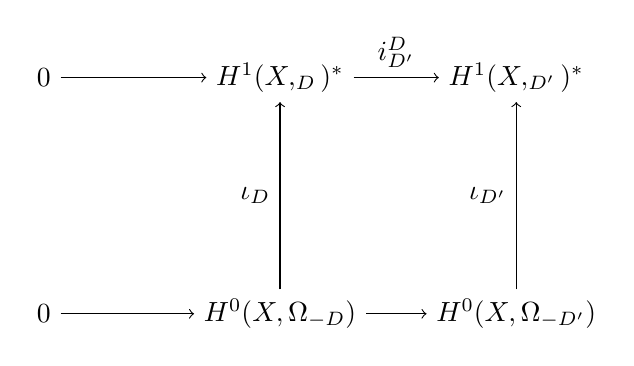
\begin{tikzpicture}[node distance=3cm, auto]
      \node (H1D) {$H^1(X, \hol_D)^\ast$};
      \node (H1D') [right of=H1D] {$H^1(X, \hol_{D'})^\ast$};
      \node (01) [left of=H1D] {0};
      \node (H0D) [below of=H1D] {$H^0(X, \Omega_{-D})$};
      \node (H0D') [right of=H0D] {$H^0(X, \Omega_{-D'})$};
      \node (02) [left of=H0D] {0};
      \draw[->] (01) to (H1D);
      \draw[->] (H1D) to node {$i_{D'}^D$} (H1D');
      \draw[->] (02) to (H0D);
      \draw[->] (H0D) to (H0D');
      \draw[->] (H0D) to node {$\iota_D$} (H1D);
      \draw[->] (H0D') to node {$\iota_{D'}$} (H1D');
    \end{tikzpicture}
  \end{center}
\end{lemma}

\begin{proof}
  Nachrechnen.\todo{Beweis das.}
\end{proof}

\begin{lemma}
  \label{lemma:urbilder}
  Sei die Notation wie in Lemma \ref{lemma:cd}. Seien weiterhin
  $\lambda \in H^1(X, \hol_D)^\ast$ und $\omega \in H^0(X,
  \Omega_{-D})$ mit $i_{D'}^D(\lambda = \iota_{D'}(\omega)$. Dann
  liegt $\omega$ bereits in $H^0(X, \Omega_{-D})$ und $\lambda =
  \iota_D (\omega)$.
\end{lemma}

\begin{proof}
  Angenommen es gelte $\omega \notin H^0(X, \Omega_{-D}) \cong
  \Omega_{-D}(X)$. Dann existierte ein $a \in X$, so dass
  $\ord_a(\omega) < D(a)$. Sei $(U_0, z)$ eine Koordinatenumgmebung
  von $a$ mit $z(a) = 0$. Auf dieser Koordinatenumgebung drücken wir
  $\omega$ durch $\omega = f \d[z]$ mit einem $f \in \mer(U_0)$
  aus. Wir können ohne Einschränkung annehmen, dass wir $U_0$ klein
  genug gewählt haben, so dass
  \begin{enumerate}
  \item $D|_{U_0 \setminus \{a\}} \equiv 0 \equiv D'|_{U_0 \setminus
      \{a\}}$ gilt und
  \item $f$ keine Null- und Polstellen auf $U_0 \setminus \{a\}$ besitzt.
  \end{enumerate}
  Nun setzen wir $U_1 := X \setminus \{a\}$, $\fu = (U_0, U_1)$ und
  $\eta = (f_0, f_1) \in C^0(\fu, \mer)$, wobei $f_0 := (zf)^{-1}$ und
  $f_1 := 0$ definiert wird. Aus $\ord_a(\omega) < D(a)$ folgte nun
  sogar, dass $\eta \in C^0(\fu, \hol_D)$ und damit sogar, dass
  \[
  \delta \eta \in Z^1(\fu, \hol) = Z^1(\fu, \hol_D) = Z^1(\fu,
  \hol_{D'})
  \]
  Bezeichnen wir mit $\xi'$ die
  Kohomologieklasse von $\delta \eta$ in $H^1(X, \hol_{D'})$ und mit
  $\xi$ die Kohomologieklasse von $\delta \eta$ in $H^1(X, \hol_D)$,
  so erhalten wir zunächst, weil $\eta \in C^0(\fu, \hol_D)$, dass
  $\xi = 0$. Nach Voraussetzung gälte nun aber
  \[
  \g{\omega}{\xi'} = \iota_{D'}(\omega)(\xi') =
  \i_{D'}^D(\lambda)(\xi') = \lambda(\xi) = 0
  \]
  Andererseits ist $\omega \eta = \left ( \frac{\d[z]}{z}, 0 \right )$
  und es folgt
  \[
  \g{\omega}{\xi'} = \res(\omega \eta) = 1
  \]
  Ein Widerspruch. Also muss $\omega \in H^0(X, \Omega_{-D})$
  gelten. Da dann $\i_{D'}^D(\lambda) = \iota_{D'}(\omega) =
  i_{D'}^D(\iota_D(\omega))$ gelten muss, folgt $\lambda =
  \iota_D(\omega)$ aus der Injektivität von $i_{D'}^D$.
\end{proof}

\begin{lemma}
  Seien $D, B \in \Div(X)$ und $X$ eine kompakte Riemannsche
  Fläche. Sei $\psi \in H^0(X, \hol_B)$. Dann induziert der
  Garbenhomomorphismus $\hol_{D-B} \xrightarrow{\psi} \hol_D$ gegeben
  durch $f \mapsto \psi f$ eine lineare Abbildung
  \[
  H^1(X, \hol_{D-B}) \ra H^1(X, \hol_D)
  \]
  und damit auch eine lineare Abbildung
  \[
  H^1(X, \hol_D)^\ast \ra H^1(X, \hol_{D-B})^\ast
  \]
  Diese bezeichnen wir auch mit $\psi$. Mit dieser Notation folgt
  $(\psi \lambda)(\xi) = \lambda(\psi \xi)$ für beliebige $\lambda \in
  H^1(X, \hol_D)^\ast$ und $\xi \in H^1(X, \hol_{D-B})$. Weiterhin
  kommutiert das folgende Diagramm
  \begin{center}
    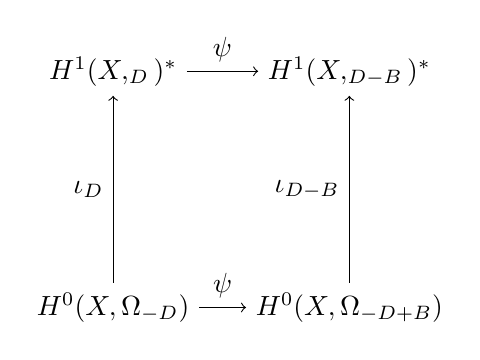
\begin{tikzpicture}
      \node (H1D) {$H^1(X, \hol_D)^\ast$};
      \node (H1B) [right of=H1D] {$H^1(X, \hol_{D-B})^\ast$};
      \node (H0D) [below of=H1D] {$H^0(X, \Omega_{-D})$};
      \node (H0B) [right of=H0D] {$H^0(X, \Omega_{-D +B})$};
      \draw[->] (H1D) to node {$\psi$} (H1B);
      \draw[->] (H0D) to node {$\psi$} (H0B);
      \draw[->] (H0D) to node {$\iota_D$} (H1D);
      \draw[->] (H0B) to node {$\iota_{D-B}$} (H1B);
    \end{tikzpicture}
  \end{center}
\end{lemma}

\begin{proof}
  Das Multiplikation mit $\psi$ ein Garbenhomomorphismus ist, ist klar
  und damit folgt die Existenz der linearen Abbildungen. Die
  Kommutativität des Diagramss erhalten wir aus der Tatsache, dass für
  beliebige $\omega \in H^0(X, \Omega_{-D})$ und $\xi \in H^1(X,
  \hol_{D-B})$ die folgende Rechnung durchführen können
  \begin{align*}
    \iota_{D-B}(\psi \omega)(\xi) = \g{\psi \omega}{\xi} = \res((\psi
    \omega) \xi) = \res(\omega (\psi \xi)) = \g{\omega}{\psi \xi} =
    \iota_D(\omega)(\psi \xi)
  \end{align*}
\end{proof}

\begin{lemma}
  \label{lemma:psi-inj}
  Falls $\psi \in H^0(X, \hol_B)$ mit $\psi \neq 0$. Dann ist $\psi:
  H^1(X, \hol_D)^\ast \ra H^1(X, \hol_{D-B})^\ast$ injektiv.
\end{lemma}

\begin{proof}
  Sei $A := (\psi) \geq -B$. Dann faktorisiert $\psi: \hol_{D-B} \ra
  \hol_D$ über $\hol_{D+A}$, d.h. das Diagramm
  \begin{center}
    \begin{tikzpicture}[node distance = 1.5cm, auto]
      \node (DB) {$\hol_{D-B}$};
      \node (D) [right of=DB] {$\hol_D$};
      \node (A) [below of=DB] {$\hol_{D+A}$};
      \draw[->] (DB) to node {$\psi$} (D);
      \draw[->] (DB) to (A);
      \draw[->, dashed] (A) to (D);
    \end{tikzpicture}
  \end{center}
  kommutiert. Weiterhin ist die Abbildung $\hol_{D+A} \ra \hol_D$ ein
  Isomorphismus, wobei die Umkehrung einfach durch Multiplikation mit
  $\psi^{-1}$ gegeben ist. Nun ist die Inklusion von $\hol_{D-B} \ra
  \hol_{D+A}$ injektiv und deshalb nach (16.8) $H^1(X, \hol_{D-B}) \ra
  H^1(X, \hol_{D+A})$ ein Epimorphismus. Also ist auch $H^1(X,
  \hol_{D-B}) \xrightarrow{\psi} H^1(X, \hol_D)$ ein Epimorphismus und
  schlussendlich die duale Abbildung injektiv. Dies zeigt die Behauptung.
\end{proof}

\begin{thm}[Der Serresche Dualitätssatz]
  Sei $D \in \Div(X)$ und $X$ eine kompakte Riemannsche Fläche. Dann
  ist $\iota_D: H^0(X, \Omega_{-D}) \ra H^1(X, \hol_D)^\ast$ ein Isomorphismus.
\end{thm}

\begin{proof}
  Aufgrund von Satz \ref{thm:iota-inj} benötigen wir nur noch die
  Surjektivität von $\iota_D$. Sei $\lambda \in H^1(X, \hol_D)^\ast$
  mit $\lambda \neq 0$ und $P \in \Div(X)$ mit $\deg P = 1$. Weiterhin
  setzen wir $D_n := D - n P$ für beliebige $n \in \N$. Als nächstes
  bezeichnen wir mit $\Lambda \subset H^1(X, \hol_{D_n})^\ast$ den
  Untervektorraum aller Linearformen der Form $\psi \lambda$, wobei
  $\psi \in H^0(X, \hol_{nP})$. Nach Lemma \ref{lemma:psi-inj} ist
  $\Lambda \cong H^0(X, \hol_{nP})$. Aus dem Satz von Riemann-Roch
  folgt damit, dass
  \[
  \dim \Lambda \geq 1 - g + n
  \]
  gilt. Aus Lemma \ref{lemma:k0} und da $\iota_{D_n}$ injektiv ist,
  erhalten wir
  \[
  \dim \im(\iota_{D_n}) = \dim H^0(X, \Omega_{-D_n}) \geq n + k_0 -
  \deg D
  \]
  Wählen wir $n > \deg D$, so erhalten wir $\deg D_n < 0$ und damit
  $H^0(X, \hol_{D_n}) = 0$. Aus dem Satz von Riemann-Roch folgt
  \[
  \dim H^1(X, \hol_{D_n})^\ast = g - 1 - \deg D_n = n + ( g - 1 -
  \deg D).
  \]
  Unter eventueller Vergrößerung von $n$ erhalten wir
  \begin{align*}
    \dim \Lambda + \dim \im(\iota_{D_n}) & \geq 1 - g + n + n + k_0 -
    \deg D \\
    & = 2 n + 1 - g + \deg D \\
    & > n + (g - 1 - \deg D) \\
    & = \dim H^1(X, \hol_{D_n})^\ast.
  \end{align*}
  Da sowohl $\Lambda$ als auch $\im(\iota_{D_n})$ Untervektorräume von
  $H^1(X, \hol_{D_n})^\ast$ sind, muss $\Lambda \cap \im(\iota_{D_n})
  \neq 0$ sein. Also existiert ein $\psi \in H^0(X, \hol_{nP})$ mit
  $\psi \neq 0$ und $\omega \in H^0(X, \Omega_{-D_n})$ mit $\psi
  \lambda = \iota_{D_n}(\omega)$. Setzen wir $A := (\psi)$, so liegt
  $\frac{1}{\psi} \in H^0(X, \hol_A)$. Zu guter Letzt erhalten wir aus
  $D' := D_n - A$, dass
  \begin{align*}
    \i_{D'}^d(\lambda) = \frac{1}{\psi} (\psi \lambda) =
    \frac{1}{\psi} \iota_{D_n}(\omega) = \iota_{D'} \left (
      \frac{1}{\psi} \omega \right )
  \end{align*}
  gilt und unter Ausnutzung von Lemma \ref{lemma:urbilder} folgt, dass
  $\omega_0 := \frac{1}{\psi} \omega \in H^0(X, \Omega_{-D})$ die
  Gleichung $\lambda = \iota_D(\omega_0)$ erfüllt.
\end{proof}

\begin{cor}
  Sei $X$ eine kompakte Riemannsche Fläche und $D \in \Div(X)$. Dann
  gilt
  \[
  \dim H^1(X, \hol_D) = \dim H^0(X, \Omega_{-D})
  \]
  Insbesondere folgt für $D = 0$
  \[
  g = \dim H^1(X, \hol) = \dim H^0(X, \Omega),
  \]
  wobei $g$ das Geschlecht von $X$ bezeichnet.
\end{cor}

%%% Local Variables: 
%%% mode: latex
%%% TeX-master: "../Bachelor"
%%% End: 




\section{Das Dirichlet Randwertproblem}
\label{sec:Dirichlet}

Es besteht ein enger Zusammenhang zwischen holomorphen und
harmonischen Abbildungen, genauer gesagt ist auf
zusammenhängenden Riemannschen Flächen jede harmonische Funktion
Realteil einer holomorphen Funktion. Dieses Resultat ist sehr
interessant, denn es ermöglicht uns holomorphe Abbildungen zu
"`konstruieren"'. Wir sind im weiteren Verlauf vor allem an
nicht-konstanten holomorphen Abbildungen interessiert und unsere
Strategie, diese Abbildungen zu finden, wird darin bestehen das
Dirichlet Randwertproblem (kurz: RWP) (vgl. Definition
\ref{defin:rwp}) zu lösen. Die Lösung eines solchen RWP ist immer
harmonisch und durch geeignete Randwerte können wir dafür sorgen, dass
sie nicht-konstant ist. Durch diesen einfachen Trick haben wir dann
ein nicht-konstante holomorphe Abbildung gefunden.

Natürlich ist per se noch nicht klar, unter welchen Umständen
überhaupt Lösungen für ein RWP existieren und ob diese eindeutig
bestimmt sind. Der Großteil des Kapitels wird sich zunächst mit etwas
Terminologie und dann der Eindeutigkeit von Lösungen des RWP
beschäftigen. Wir werden Perrons Methode (Lemma \ref{lemma:perron})
verwenden, um Lösungskandidaten zu konstruieren und schlussendlich ein
hinreichendes Kriterium angeben, um Gebiete auf denen Lösungen des RWP
existieren zu identifizieren.

Im weiteren bezeichne $X$ immer ein Riemannsche Fläche.

\begin{defin}
  Für jedes $\omega \in \diff^{(1)}(X)$ existiert genau ein $\omega_1
  \in \diff^{1,0}(X)$ und genau ein $\omega_2 \in \diff^{0,1}(X)$, so
  dass $\omega = \omega_1 + \omega_2$ gilt. Dies ermöglicht die
  Definition der Abbildung
  \[
  \ast : \diff^{(1)}(X) \ra \diff^{(1)}(X), \quad \omega_1 + \omega_2
  \mapsto i(\bar \omega_1 + \bar \omega_2).
  \]
\end{defin}

\begin{prop}
  Die Abbildung $\ast$ ist ein $\R$-linearer Isomorphismus. Weiterhin
  bildet er $\diff^{1,0}(X)$ auf $\diff^{0,1}(X)$ ab und umgekehrt.
\end{prop}

\begin{proof}
  Die $\R$-Linearität von $\ast$ ist klar. Die Bijektivität folgt aus
  der Tatsache, dass $\ast^{-1} = - \ast$ gilt. Sei nun weiterhin
  $\omega \in \diff^{1,0}(X)$. Auf einer Karte $(z,U)$ nimmt $\omega$
  dann die Form $\omega = f \d[z]$ für ein $f \in \diff(U)$ an. Dann gilt
  aber $\ast \omega = i \bar \omega = i \bar f \d[\bar z] \in
  \diff^{0,1}(X)$ auf der Karte. Also wird tatsächlich
  $\diff^{1,0}(X)$ auf $\diff^{0,1}(X)$ abgebildet. Die Bijektivität
  folgt auch einfach wieder aus der Tatsache, dass $\ast^{-1} = -
  \ast$ gilt.
\end{proof}

\begin{defin}
  Eine 1-Form $\omega \in \diff^1(X)$ heißt \init{harmonisch}, falls
  \[
  \d[\omega] = 0 = \d[\ast \omega]
  \]
  gilt.
\end{defin}

\begin{thm}
  \label{thm:harm-form}
  Jede reelle 1-Form $\sigma \in \diff^1(X)$ ist Realteil genau einer
  holomorphen 1-Form $\omega \in \Omega(X)$.
\end{thm}

\begin{proof}
  Wie können $\sigma = \omega_1 + \omega_2$ mit $\omega_1 \in
  \diff^{1,0}(X)$ und $\omega_2 \in \diff^{0,1}(X)$ schreiben. Nun
  folgt aber aus $\d[\omega] = 0$, dass
  \begin{align}
    \d[''\omega_1] + \d['\omega_2] = 0 \label{eq:harm1}
  \end{align}
  gilt und aus $\d[\ast \omega] = 0$, dass
  \begin{align}
  i(\d['\bar \omega_1] - \d[''\bar \omega_2]) = 0 \label{eq:harm2}
  \end{align}
  gilt. Durch eine einfache
  Rechnung auf Karten lässt sich \eqref{eq:harm2} zu
  \[
  0 = \overline{\d[''\omega_1]} - \overline{\d['\omega_2]}
  \]
  umformen. Dies liefert uns zunächst zusammen mit
  Gleichung\eqref{eq:harm1}, dass $\d[''\omega_1] = 0$ und $\d['\omega_2] = 0$
  gelten. Daraus folgt aber direkt, dass $\omega_1 \in \Omega(X)$
  gilt. Und unter Ausnutzung, von $\overline{\d['\omega_2]} = \d[''
  \bar \omega_2]$ erhalten wir, dass $\bar \omega_2 \in \Omega(X)$
  gilt. Nun wissen wir aber, dass $\sigma$ reell ist und wir erhalten
  die Gleichung
  \[
  \omega_1 + \omega_2 = \sigma = \bar \sigma = \bar \omega_1 + \bar
  \omega_2.
  \]
  Da die Darstellung von $\sigma$ eindeutig ist, muss $\omega_1 =
  \bar \omega_2$ gelten. Setzen wir $\omega = 2\omega_1 \in
  \Omega(X)$, so gilt
  \begin{align*}
    \Re(\omega) & = \Re(2\omega_1) = \frac{1}{2}( 2 \omega_1 + 2 \bar
    \omega_1) = \omega_1 + \omega_2 = \sigma.
  \end{align*}
  Um nun die Eindeutigkeit von $\omega$ zu beweisen, zeigen wir, dass
  $\sigma = 0$ bereits $\omega = 0$ impliziert. Dies genügt, da
  $\Re(x) = \Re(y)$ genau dann gilt, wenn $\Re(x-y) = 0$ ist. Dies
  folgt aus der $\R$-Linearität von $\Re$ \footnote{Wobei $\Re$
  natürlich nicht $\C$ linear ist.}. Sei also $\omega \in \Omega(X)$
  mit $\Re(\omega) = 0$. Nun existiert aber lokal immer eine
  Stammfunktion für $\omega$, d.h. lokal existiert ein holomorphes
  $f$, so dass $\omega = \d[f]$ gilt. Dann folgt aber, dass
  $\d[\Re(f)] = 0$ sein muss, also ist $\Re(f)$ konstant. Das wiederum
  hat aber zur Folge, dass die holomorphe Funktion $e^f$ ihr
  Betragsmaximum annimmt, denn es gilt $|e^f| = e^{\Re(f)}$. Dann ist
  aber $e^f$ nach dem Maximumsprinzip für holomorphe Funktionen
  (vgl. \cite[Kor. 2.6]{For})
  konstant. Also ist auch $f$ konstant und es gilt $\omega = \d[f] =
  0$. Da dies lokal um jeden Punkt gilt, ist somit $\omega = 0$ und
  damit ist unser $\omega$ eindeutig bestimmt.
\end{proof}

\begin{defin}
  Sei $Y \subset X$ offen und $X$ eine Riemannsche Fläche. Dann heißt
  $u \in \diff(Y)$ \init{harmonisch}, falls $\d['\d[''u]] = 0$ gilt.
  In lokalen Koordinaten $(z,U)$ mit $z = x + iy$ bedeutet das
  \begin{align*}
    \Delta u = \left ( \frac{\partial^2}{\partial x^2} +
      \frac{\partial^2}{\partial y^2} \right ) u = 4
    \frac{\partial^2}{\partial z \partial \bar z} u = 0.
  \end{align*}
\end{defin}

\begin{prop}
  \label{prop:harm-realteil-hol}
  Sei $G \subset X$ ein Gebiet, $X$ eine Riemannsche Fläche
  und $u: G \ra \R$ harmonisch. Dann existiert ein $f \in \hol(G)$, so dass
  \[
  u = \Re(f)
  \]
  gilt.
\end{prop}

\begin{proof}
  Nach Satz \ref{thm:harm-form} gilt
  \begin{align*}
    \d[\d[u]] = 0 \quad \text{und} \quad \d[\ast\d[u]] = 0.
  \end{align*}
  Also existiert ein $\omega \in \Omega(G)$, so dass $\d[u] =
  \Re(\omega)$. Nun ist aber $G$ einfach zusammenhängend, d.h. es gibt
  eine Funktion $g \in \hol(G)$, so dass $\omega = \d[g]$. Damit ist
  $\d[u] = \Re(\d[g])$ und es folgt $u = \Re(g) +$const.
\end{proof}

\begin{rem}
  Die Umkehrung gilt immer, d.h. der Realteil einer holomorphen
  Funktion ist immer harmonisch.
\end{rem}

\begin{prop}[Maximumsprinzip für harmonische Funktione]
  \label{prop:max-prinzip-harm}
  Sei $Y \subset X$ ein Gebiet. Sei weiterhin $u: Y \ra \R$ harmonisch
  und $x_0 \in Y$ mit $u(x_0) = \sup_{y \in Y} u(y)$. Dann ist $u$ konstant.
\end{prop}

\begin{proof}
  Wir verwenden für den Beweis ein
  "`Offen-Abgeschlossen"'-Argument. Sei dazu
  \[
  M:= \{ y \in Y| u(y) = u(x_0)\} \neq \varnothing.
  \]
  Wir behaupten zunächst, dass $M$ offen ist.
  Sei $y \in Y$. Dann existiert eine offene,
  einfachzusammenhängende Umgebung $U \subset Y$ von $y$. 
  Nach Proposition \ref{prop:harm-realteil-hol} folgt dann die
  Existenz von $f \in \hol(U)$ mit $u|_U = \Re(f)$.
  Weiterhin ist die reelle Exponentialfunktion streng monoton
  steigend und somit nimmt die Funktion $e^u$ bei $y$ ein Maximum
  an. Allerdings gilt auch $|e^f| = e^u$, was nichts anderes
  bedeutet, als dass die holomorphe Funktion $e^f$ ein
  Betragsmaximum bei $y$ annimmt. 
  Aus dem Maximumsprinzip für holomorphe Funktionen (vgl. \cite[Kor. 2.6]{For}) folgt dann die
  Konstanz von $e^f$ und damit
  \[
  u|_U \equiv \text{const.}
  \]
  Also gilt $y \in U \subset M$.
  
  Als nächstes behaupten wir, dass $M$ zusätzlich auch abgeschlossen
  ist. Dies ist aber eine direkte Konsequenz aus der Stetigkeit von $u$.

  Damit ist $M \subset Y$ sowohl offen als auch abgeschlossen und da
  $Y$ zusammenhängend ist, muss $M$ entweder leer oder ganz $Y$
  sein. Nun liegt $x_0 \in M$ und somit folgt $M = Y$, also ist $u$ konstant.
\end{proof}

\begin{defin}
  \label{defin:rwp}
  Sei $Y\subset X$ offen, $X$ eine Riemannsche Fläche und $f: \partial
  Y \ra \R$ stetig. Man nennt $u \in C(\bar Y, \R)$ \init{Lösung des Dirichlet
    Randwertproblemes} (Dirichlet-RWP), falls
  \begin{enumerate}
  \item $u|_Y$ harmonisch ist und
  \item $u|_{\partial Y} \equiv f$.
  \end{enumerate}
\end{defin}

\begin{prop}
  \label{prop:dirichlet-eindeutig}
  Sei $Y \Subset X$ offen und $\partial Y \neq \varnothing$. Dann ist
  daie Lösung eines Dirichlet-RWP eindeutig, falls sie existiert.
\end{prop}

\begin{proof}
  Seien $u_1, u_2$ zwei Lösungen des Dirichlet-Problems. Dann erfüllen
  die Funktionen
  \[
  (u_1 - u_2)|_{\partial Y} \equiv (u_2 - u_1)|_{\partial Y} \equiv 0
  \]
  und sind harmonisch. Aus dem Maximumsprinzip folgt sofort, die
  Nicht-Positivität von sowohl $u_1 - u_2$ als auch von $u_2 - u_1$
  auf allen Zusammenhangskomponenten von $Y$, also folgt
  \[
  0 \leq u_1 - u_2 \leq 0
  \]
  und damit
  \[
  u_1 \equiv u_2.
  \]
\end{proof}

\begin{thm}
  \label{thm:poisson}
  Sei $f: \partial B_R(0) \ra \R$ stetig, $R > 0$ und
\begin{align*}
    u(z) :=
    \begin{cases}
      \frac{1}{2\pi} \int_0^{2\pi} \frac{R^2 - |z|^2}{|Re^{i\phi}
        - z|^2} f(R e^{i\phi}) \d[\phi] & \text{für } |z| < R\\
      f(z) & \text{für } |z| = R
    \end{cases}
  \end{align*}
  Dann ist $u$ stetig auf $\overline{B_R(0)}$ und harmonisch auf $B_R(0)$;
  löst also das Dirichlet-Problem auf $\overline{B_R(0)}$.
\end{thm}

\begin{proof}
  Für $z \neq \rho$ definieren wir
  \[
  P(z, \rho) := \frac{|\rho|^2 - |z|^2}{|\rho - z|^2}, \qquad
  F(z,\rho) := \frac{\rho +z }{\rho - z}
  \]
  Dann gilt $P(z, \rho) = \Re(F(z, \rho))$ und für $u$ ergibt sich
  \begin{align*}
    u(z) & = \frac{1}{2\pi} \int_0^{2\pi} P(z, Re^{i\phi})
    f(Re^{i\phi}) \d[\phi] \\
    & = \Re \left ( \frac{1}{2\pi} \int_0^{2\pi} F(z, Re^{i\phi})
      f(Re^{i\phi}) \d[\phi] \right ).
  \end{align*}
  Nun ist $F$ als Funktion von $z$ holomorph (falls $z \neq \rho$)
  und damit erhalten wir aus der Leibnizregel, dass $u$ der Realteil
  einer holomorphen Funktion ist, also harmonisch.
  
  Als nächstes müssen wir die Stetigkeit von $u$ auf dem Rand
  zeigen. Zunächst zeigen wir jedoch die Gleichung
  \[
  \frac{1}{2\pi} \int_0^{2\pi} P(z, Re^{i\phi}) \d[\phi] = 1.
  \]
  Dazu verwenden wir den Residuensatz, denn es gilt
  \begin{align}
  \frac{1}{2\pi} \int_0^{2\pi} P(z, Re^{i\phi}) \d[\phi]
  = \Re \left ( \frac{1}{2\pi i} \int_{|\rho| = R} \underbrace{
      \frac{\rho + z}{(\rho - z)\rho}}_{=:h_z(\rho)} \d[\rho] \right
  ). \label{eq:residuensatz}
  \end{align}
  Weiterhin ist $\res_{\rho = z} h_z(\rho) = 2$ und $\res_{\rho=0}
  h_z(\rho) = -1$. Da jede Singularität nur einmal umlaufen wird
  erhalten wir
  \[
  \eqref{eq:residuensatz} = \Re(\res_{z = \rho}h_z(\rho) + \res_{z =
    0} h_z(\rho)) = 1.
  \]
  Also gilt für $\rho_0 \in \partial B_R(0)$ und $z \in B_R(0)$
  \[
  u(z) - f(\rho_0) = \frac{1}{2\pi} \int_0^{2\pi} P(z, \rho) (f (\rho)
  - f(\rho_0) )\d[\phi],
  \]
  wobei $\rho = Re^{i\phi}$ gesetzt wurde. Sei nun $\epsilon > 0$ beliebig. Da $f$
  stetig ist existiert ein $\delta_0 > 0$, so dass
  \[
  |f(\rho) - f(\rho_0)| \leq \frac{\epsilon}{2} \qquad \forall |\rho -
  \rho_0| \leq \delta_0, \quad \rho, \rho_0 \in \partial B_R(0)
  \]
  gilt. Weiterhin existiert ein $M > 0$, so dass $|f(\rho)| \leq M$ für
  jedes $\rho \in \partial B_R(0)$ ist. Setzen wir $\alpha \subset [0, 2\pi]$
  so, dass
  \[
  |R e^{i\phi} - \rho_0| \leq \delta_0 \qquad \forall \phi \in \alpha
  \]
  und $\beta := [0, 2\pi]\setminus \alpha$, so erhalten wir
  \begin{align*}
    |u(z) - f(\rho_0)| & \leq \frac{1}{2\pi} \int_\alpha
    \underbrace{P(z, \rho)}_{\geq 0} \frac{\epsilon}{2} \d[\phi] +
    \frac{1}{2\pi} \int_\beta P(z, \rho) 2 M \d[\phi] \\
    & \leq \frac{\epsilon}{2} + \frac{M}{\pi} \int_\beta P(z,
    Re^{i\phi}) \d[\phi].
  \end{align*}
  Sei nun $|z - \rho_0| =: \delta \leq \frac{\delta_0}{2}$. Dann gilt
  für $\phi \in \beta$
  \[
  |Re^{i\phi} - z| \geq |Re^{i\phi} - \rho_o| - |z - \rho_o| \geq
  \delta_0 - \frac{\delta_0}{2} = \frac{\delta_0}{2}
  \]
  und damit für $P$
  \[
  P(z, Re^{i\phi}) = \frac{(R+ |z|)(R - |z|)}{|Re^{i\phi} - z|^2} \leq
  \frac{4 \cdot 2 R \delta}{\delta_0^2}.
  \]
  Insgesamt erhalten wir
  \[
  |u(z) - f(\rho_0)| < \frac{\epsilon}{2} + \frac{8 R
    \delta}{\delta_0^2} \cdot \frac{M}{\pi} \cdot 2\pi
  \]
  und damit wird auch der rechte Summand kleiner als
  $\frac{\epsilon}{2}$, wenn $\delta =: |z - \rho_0|$ klein genug
  gewählt wurde.
\end{proof}

\begin{cor}
  \label{cor:harm-darstellung}
  Sei $u: B_R(0) \ra \R$ harmonisch, $ R > 0$. Dann gilt
  \[
  u(z) = \frac{1}{2\pi} \int_0^{2\pi} \frac{r^2 - |z|^2}{|re^{i\phi} -
    z|^2} u(re^{i\phi}) \d[\phi]
  \]
  für jedes $|z|<r<R$.
\end{cor}

\begin{proof}
  Die Aussage folgt direkt aus Satz \ref{thm:poisson} und Proposition \ref{prop:dirichlet-eindeutig}.
\end{proof}

\begin{cor}
  \label{cor:harm-konvergenz}
  Sei $(u_n)_{n\in \N} \subset C(B_r(0), \R)$ eine folge harmonischer
  Funktionen, die kompakt gegen
  \[
  u: B_R(0) \ra \R
  \]
  konvergieren. Dann ist $u$ bereits harmonisch.
\end{cor}

\begin{proof}
  Nach Korollar \ref{cor:harm-darstellung} erhalten wir für jedes $|z|
  < r <R$
  \[
  u_n(z) = \frac{1}{2\pi} \int_0^{2\pi} P(z, re^{i\phi})
  u_n(re^{i\phi}) \d[\phi]
  \]
  Da $u_n$ gleichmäßig auf $\partial B_r(0)$ konvergiert, gilt die
  Integralformel auch für $u$. Damit ist $u$ auf allen $B_r(0)$ mit $r <
  R$ und schlußendlich auf $B_R(0)$ harmonisch.
\end{proof}

\begin{thm}[Harnacksches Prinzip für Kreisscheiben]
  \label{thm:harnack}
  Sei $M \in \R$ und $u_0 \leq u_1 \leq \dots \leq M$ eine monoton
  wachsende, beschränkte Folge harmonischer Funktionen von $B_R(0)$ nach
  $\R$. Dann konvergiert $(u_n)_{n\in \N}$ kompakt gegen eine harmonische
  Funktion $u: B_R(0) \ra \R$.
\end{thm}

\begin{proof}
  Sei $K \subset B_R(0)$ kompakt. Dann existieren $\rho < r < R$, so
  dass $K \subset \overline{B_\rho(0)}$. Sei $\epsilon > 0$ gegeben und
  \[
  \epsilon' := \epsilon \frac{r - \rho}{ r+ \rho} > 0.
  \]
  Nun ist $(u_n(0))_{n \in \N}$ eine monoton wachsende Folge und
  beschränkt, d.h. es existiert ein $N \in \N$, so dass
  \[
  u_n(0) - u_m(0) \leq \epsilon' \qquad \forall n \geq m \geq N
  \]
  gilt. Für $|z| \leq \rho$ erhalten wir
  \begin{align}
    0 \leq P(z, re^{i\phi}) & = \frac{(r - |z|)(r+|z|)}{|re^{i\phi} -
      z|^2} \nonumber\\
    & \leq \frac{(r- |z|)(r + |z|)}{(r - |z|)^2} \nonumber\\
    & = \frac{r + |z|}{r - |z|} \nonumber\\
    & \leq \frac{ r + \rho}{ r - \rho} \label{eq:P-absch} 
  \end{align}
  Für beliebige $z \in K$ gilt nun die folgende Integralformel
  \begin{align*}
    u_n(z) - u_m(z) & = \frac{1}{2\pi} \int_0^{2\pi} P(z, re^{i\phi}
    (u_n(re^{i\phi}) - u_m(re^{i\phi})) \d[\phi] \\
    & \stackrel{\eqref{eq:P-absch}}{\leq} \frac{r + \rho}{r - \rho}
    \frac{1}{2\pi} \int_0^{2\pi} (u_n(r e^{i\phi} u_m(re^{i\phi})
    \d[\phi] \\
    & = \frac{r+\rho}{r - \rho} (u_n(0) - u_m(0)) \\
    & \leq \epsilon.
  \end{align*}
  Also konvergiert $(u_n)_{n \in \N}$ kompakt und nach Korollar
  \ref{cor:harm-konvergenz} ist die Grenzfunktion wieder harmonisch.
\end{proof}

\begin{prop}
  \label{prop:harm-rf}
  Sei $X$ eine Riemannsche Fläche und $D \Subset U \subset X$, so dass
  $(z, U)$ eine Karte und $z(D) \subset \C$ eine Kreisscheibe
  ist. Dann ist das Dirichlet-Problem auf $D$ wohldefiniert und
  eindeutig lösbar.
\end{prop}

\begin{proof}
  Die Aussage folgt daraus, dass die Eigenschaft harmonisch zu sein
  invariant unter biholomorphen Transformationen und damit unabhängig
  von der gewählten Kartenabbildung ist. Die Lösung lässt sich dann
  einfach auf $z(D)$ nach Satz \ref{thm:poisson} ermittlen.
\end{proof}

\begin{defin}
  Sei $X$ eine Riemannsche Fläche und $Y \subset X$ offen. Wir
  bezeichnen mit $\Reg(Y)$ die Menge aller Teilgebiete $D \Subset
  Y$, die den Voraussetzungen von Propositon \ref{prop:harm-rf}
  genügen.
  
  Für $u \in C(Y, \R)$ und $D \in \Reg(Y)$ definieren wir $P_D u: Y
  \ra \R$ durch $P_D u |_{Y \setminus D} \equiv u_{Y \setminus D}$ und
  $P_Du|_D$ ist die Lösung des Dirichlet-Problems mit Randwerten
  $u|_{\partial D}$.
\end{defin}

\begin{cor}
  \label{cor:pd-rechenregeln}
  Mit der gleichen Notation wie in der vorherigen Definition erhalten wir
  für beliebige $u, v\in C(Y, \R)$ und $\lambda \in \R$:
  \begin{enumerate}
  \item $P_D(u+v) = P_Du + P_D v$,
  \item $P_D(\lambda u) = \lambda P_D u$ und
  \item $u \leq v \Ra P_Du \leq P_D v$.
  \end{enumerate}
\end{cor}

\begin{proof}
  Die ersten beiden Aussagen ergeben sich direkt aus der Eindeutigkeit
  harmonischer Funktionen und 3. ist eine Folge des Maximumprinzips.
\end{proof}

\begin{cor}
  $u \in C(Y, \R)$ ist genau dann harmonisch, wenn $P_Du = u $ für
  jedes $D \in \Reg(Y)$
\end{cor}

\begin{proof}
  \begin{description}
  \item[$\Ra$] Diese Richtung ergibt sich direkt aus der Definition.
  \item[$\La$] Folgt aus der Tatsache, dass harmonisch zu sein eine
    lokale Eigenschaft ist und es zu jedem Punkt $x \in Y$ ein $D \in
    \Reg(Y)$ mit $x \in D$ existiert.
  \end{description}
\end{proof}

\begin{defin}
  Sei $Y \subset X$ offen und $X$ eine Riemannsche Fläche.
  Ein $u \in C(Y, \R)$ heißt
  \begin{enumerate}
  \item \init{subharmonisch}, falls $P_D u \geq u$ für jedes $D \in \Reg(Y)$.
  \item \init{lokal subharmonisch}, falls es zu jedem Punkt in $Y$
    eine Umgebung gibt, auf der $u$ subharmonisch ist.
  \end{enumerate}
\end{defin}
\begin{cor}
  Sei $Y \subset X$ offen und $X$ eine Riemannsche Fläche. Seien
  weiterhin $u,v \in C(Y, \R)$ subharmonisch und $\lambda \geq
  0$. Dann sind $u+v$, $\lambda u$ und $\sup(u,v)$ subharmonisch.
\end{cor}

\begin{proof}
  $u+v$ und $\lambda u$ folgen direkt aus Korollar
  \ref{cor:pd-rechenregeln}. Um die Aussage für $\sup(u,v)$ zu zeigen,
  betrachten wir zunächst eine beliebige Funktion $f \in C(\partial D,
  \R)$. Dann gilt klarerweise $f \leq |f|$. Seien nun $\tilde u$ und
  $\tilde v$ Lösungen des Randwertproblem zu $f$ bzw. $|f|$. Dann
  folgt aus dem Maximumprinzip, dass $\tilde u \leq \tilde v$ gelten
  muss. Andererseits gilt auch $-f \leq |f|$ und aus der Eindeutigkeit
  der harmonischen Funktionen und dem Maximumprinzip erhalten wird $-
  \tilde u \leq \tilde v$. Insgesamt gilt also $|\tilde u| \leq \tilde
  v$. Diese Aussage verwenden wir, um die folgende Abschätzung herzuleiten
  \begin{align*}
    P_D \sup(u,v) & = \frac{1}{2} ( P_D u + P_D v + P_D|u - v|) \\
    & \geq \frac12 (P_D u + P_D v + |P_D u - P_D v|) \\
    & = \sup(P_D u, P_D v) \\
    & \geq \sup(u,v).
  \end{align*}
  Also ist auch $\sup(u,v)$ subharmonisch.
\end{proof}

\begin{thm}[Maximumprinzip für lokal subharmonische Funktionen]
  Sei $Y \subset X$ ein Gebiet, $X$ eine Riemannsche Fläche und $u
  \in C(Y, \R)$ lokal subharmonisch, so dass ein $x_0 \in Y$ existiert
  mit
  \[
  u(x_0) = \sup_{y\in Y} u(y)
  \]
  Dann ist $u$ konstant.
\end{thm}

\begin{proof}
  Sei $M:= \{y \in Y | u(y) = u(x_0) =: c \}$. Angenommen es gälte $M \neq
  Y$. Dann existierte ein $a \in \partial M$ und aus der Stetigkeit
  von $u$ folgte $u(a) = u(x_0)$. Nun müsste in jeder Umgebung von $a$
  ein $x$ existieren, so dass $u(x) < u(x_0)$ wäre, d.h. wir könnten ein
  $D \in \Reg(y)$ finden mit $a \in D$ und $u|_{\partial D} \not
  \equiv c$. Wenn wir nun $D$ klein genug wählen, können wir annehmen, dass $u$
  subharmonisch in einer Umgebung von $\bar D$ ist. Also gilt $u \leq
  P_D u =: v$. Damit ist $v$ harmonisch auf $D$ und $v|_{\partial D} \equiv
  u|_{\partial_D} \leq c$ und es folgt $v \leq c$ auf $\bar D$, aber
  $c = u(a) \leq v(a)$. $v$ nimmt also ihr Maximum im Inneren an und
  ist nach Proposition \ref{prop:max-prinzip-harm} konstant,
  insbesondere wäre $v \equiv c$ auf $\partial D$. Dies ist ein Widerspruch zu
  $u|_{\partial D} \not \equiv c$. Also muss $M = Y$ gelten.
\end{proof}

\begin{cor}
  Sei $Y\subset X$ offen, $X$ eine Riemannsche Fläche und $u \in C(Y,
  \R)$ lokal subharmonisch. Dann ist $u$ bereits subharmonisch.
\end{cor}

\begin{proof}
  Sei $D \in \Reg(Y)$ beliebig. Da $P_D u$ harmonisch auf $D$ ist, ist
  $v:= u- P_Du$ lokal subharmonisch auf $D$ und $v|_{\partial D}
  \equiv 0$. Also folgt aus dem Maximumprinzip $v \leq0$ auf $D$ und
  damit $P_Du \geq u$.
\end{proof}

\begin{lemma}
  Sei $u \in C(Y, \R)$ subharmonisch und $B \in \Reg(Y)$. Dann ist
  $P_B u$ auch subharmonisch.
\end{lemma}

\begin{proof}
  Wir setzen $v:= P_B u$ und wählen $D \in \Reg(Y)$ beliebig. Wir
  zeigen dann die Abschätzung $P_D v \geq v$. Auf $Y \setminus D$ gilt $P_Dv \equiv v$
  und auf $Y\setminus B$ gilt
  \[
  P_Dv \equiv P_DP_Bu = P_Du \geq u = P_Bu = v
  \]
  Damit gilt $v - P_Dv \leq 0$ auf $Y \setminus (B \cap D)$,
  insbesondere $v- P_D v \leq 0$ auf $\partial (Y \setminus (B \cap
  D))$ und aus dem Maximumprinzip für harmonische Funktionen folgt $v
  - P_D v \leq 0$ auf $B \cap D$, da $v - P_D v$ dort harmonisch
  ist. Insgesamt ergibt sich $P_Dv \geq v$ auf ganz $Y$.
\end{proof}

\begin{lemma}[Perron]
  \label{lemma:perron}
  Sei $M \subset C(Y, \R)$ eine nicht-leere Menge subharmonischer
  Funktionen mit den folgenden Eigenschaften:
  \begin{enumerate}
  \item $u,v \in M \Ra \sup(u,v) \in M$,
  \item $u \in M, D \in \Reg(Y) \Ra P_Du \in M$ und
  \item $\exists K \in \R: u \leq K \quad \forall u \in M$.
  \end{enumerate}
  Dann ist die Funktion $u^\ast : Y \ra \R$ durch $u^\ast(x) :=
  \sup\{u(x) \mid u \in M \}$ harmonisch auf $Y$.
\end{lemma}

\begin{proof}
  Sei $a \in Y$ und $D \in \Reg(Y)$ eine Umgebung von $a$. Sei
  weiterhin $(u_n)_{n \in \N} \subset M$ mit $\lim_{n \ra \infty}
  u_n(a) = u^\ast(a)$. Aufgrund von 1. können wir ohne Einschränkung davon ausgehen, dass
  $u_0 \leq u_1 \leq u_2 \leq \dots$ ist. Setzen wir $v_n := P_D u_n$, so gelten
  \begin{align}
   & u_n \leq v_n \leq u^\ast \label{eq:v-absch} & \text{ und }\\
   & v_0 \leq v_1 \leq v_2 \leq \dots \nonumber
  \end{align}
  Nach dem Harnackschen Prinzip konvergiert $(v_n)_{n \in \N}$ auf $D$
  gegen eine harmonische Funktion $v: D \ra \R$ und aus
  \eqref{eq:v-absch} erhalten wir $v(a) = u^\ast(a)$ und $v \leq
  u^\ast$ auf $D$.
  
  Wir zeigen zunächst, dass $v \equiv u^\ast|_D$ gilt. Sei dazu $x \in
  D$ beliebig und $(w_n)_{n\in \N}\subset M$ mit
  $\lim_{n \ra \infty}w_n(x) = u^\ast(x)$. Aufgrund von 1. und
  2. können wir $v_n \leq w_n = P_D w_n$ und $w_n
  \leq w_{n+1}$ annehmen. Also konvergiert $(w_n)_{n \in \N}$ auf $D$
  gleichmäßig gegen $w: D \ra \R$ mit $v \leq w \leq u^\ast$. Damit
  gilt aber $u^\ast(a) = v(a) \leq w(a) \leq u^\ast(a)$ und aus
  dem Maximumprinzip angewandt auf $v-w$ ergibt sich $v \equiv w$ auf
  $D$. Insbesondere $v(x) = w(x) = u^\ast(x)$. Also ist $u^\ast = v$
  harmonisch auf $D$ und da $D$ beliebig gewählt
  war auf ganz $Y$.
\end{proof}

\begin{defin}
  \label{def:perron}
  Sei $Y \subset X$ offen, $\partial Y \neq \varnothing$ und
  $f: \partial Y \ra \R$ stetig und beschränkt. Setzen wir $K :=
  \sup\{f(x) : x \in \partial Y\}$, dann bezeichnet
  $\pe_f$ die Menge aller $u \in C(\bar Y, \R)$, so dass
  \begin{enumerate}
  \item $u|_Y$ subharmonisch ist und
  \item $u|_{\partial Y} \leq f$ und $u \leq K$ gilt.
  \end{enumerate}
  $\pe_f$ wird als \init{Perronklasse} von $f$ bezeichnet.
\end{defin}

\begin{cor}
  Mit der Notation aus Definition \ref{def:perron} folgt, dass $u^\ast := \sup_{u
    \in \pe_f} u$ harmonisch auf $Y$ ist.
\end{cor}

\begin{proof}
  Wir wenden einfach Lemma \ref{lemma:perron} auf $M := \pe_f$ an.
\end{proof}

\begin{rem}
  Damit $u^\ast$ eine Lösung des Dirichlet-Problems auf $Y$ ist,
  müsste
  \begin{align}
  \lim_{\substack{y\ra x\\y \in Y}}u^\ast(y) =
  f(x) \label{eq:dirichlet-rand} 
  \end{align}
  für jedes $x \in \partial Y$ gelten. Dies ist leider nicht immer der
  Fall. Im folgenden wollen wir Kriterien für die Randpunkte angeben,
  die sicherstellen, dass \eqref{eq:dirichlet-rand} erfüllt wird.
\end{rem}

\begin{defin}
  Sei $Y \subsetneq X$ offen und $X$ eine Riemannsche Fläche. Ein
  Punkt $x \in \partial Y$ heißt \init{regulär}, falls es eine
  offene Umgebung $U \subset X$ von $x$ und eine Funktion $\beta  \in
  C(\bar Y \cap U)$ existiert, so dass
  \begin{enumerate}
  \item $\beta|_{Y \cap U}$ harmonisch ist,
  \item $\beta(x) =0$ und $\beta(y) < 0$ für beliebige $y \in \bar Y
    \cap U \setminus \{x\}$ gilt.
  \end{enumerate}
  $\beta$ wird als \init{Barriere} von $x$ bezeichnet.
\end{defin}

\begin{lemma}
  \label{lemma:zsh-komp}
  Sei $X$ eine Riemannsche Fläche, $Y \subset X$ eine offene Menge und
  $Z \subset Y$ eine Zusammenhangskomponente von $Y$. Dann ist $Z$ offen.
\end{lemma}

\begin{proof}
  Sei $x \in Z$. Dann finden wir eine offene, zusammenhängende
  Koordinatenumgebung $U \subset Y$ mit mit $x \in U$. Nun ist aber
  $Z$ die maximale zusammenhängende Teilmenge, die $x$ enthält und da
  $U$ auch zusammenhängend gewählt wurde, muss $U \subset Z$
  gelten. Also ist $x$ ein innerer Punkt und damit $Z$ offen.
\end{proof}

\begin{cor}
  Sei $x \in \partial Y$ ein regulärer Randpunkt und $Z \subset Y$
  offen mit $x \in \partial Z$.\\
  Dann ist $x$ ein regulärer Randpunkt von $Z$. Insbesondere hat jede
  Zusammenhangskomponente von $Y$ regulären Rand.
\end{cor}

\begin{lemma}
  \label{lemma:regulär-trennen}
  Sei $x \in \partial Y$ ein regulärer Randpunkt und $V$ eine offene
  Umgebung von $x$ mit reellen Konstanten $m \leq c$. Dann existiert
  ein $v \in C( \bar Y, \R)$, so dass die folgenden Eigenschaften
  \begin{enumerate}
  \item $v|_Y$ ist subharmonisch,
  \item es gelten $v(x) = c$ und $v|_{\bar Y \cap V} \leq c$ und
  \item $v|_{\bar Y\setminus V} \equiv m$
  \end{enumerate}
  erfüllt sind.
\end{lemma}

\begin{proof}
  Wir können ohne Einschränkung $c = 0$ annehmen. Sei $U$ eine offene Umgebung von $x$ mit Barriere $\beta \in C(\bar
  Y \cap U, \R)$. Wir können nun eine offene Umgebung $\tilde V \Subset U \cap V$
  von $x$ finden. Dort gilt
  \[
  \sup\{\beta(y)| y \in \partial \tilde V \cap \bar Y \} < 0.
  \]
  Also existiert ein $k > 0$, so dass $k\beta|_{\partial \tilde V \cap
    \bar Y} < m$.
  Schlußendlich definieren wir
  \[
  v :=
  \begin{cases}
    \sup(m, k\beta) & \text{auf } \bar Y \cap \tilde V\\
    m & \text{auf } \bar Y \setminus V
  \end{cases}.
  \]
  Damit ist $v$ stetig und genügt den Bedingungen 1 bis 3.
\end{proof}

\begin{lemma}
  Sei $Y \subsetneq X$ offen, $f \in C(\partial Y, \R)$ beschränkt und
  $u^\ast := \sup_{u \in \pe_f}u$, wobei $\pe_f$ die Perronklasse von
  $f$ bezeichnet. Dann gilt für jeden regulären Randpunkt $x \in \partial Y$
  \[
  \lim_{\substack{y \ra x\\y \in Y}} u^\ast(y) = f(x).
  \]
\end{lemma}

\begin{proof}
  Sei $\epsilon > 0$ beliebig. Dann existiert eine relativ kompakte offene
  Umgebun $V$ von $x$ mit
  \[
  f(x) - \epsilon \leq f(y) \leq f(x) + \epsilon \qquad \forall y
  \in \partial Y \cap V
  \]
  Seien $k, K \in \R$ mit $k \leq f(y) \leq K$ für jedes $y
  \in \partial Y$.
  \begin{description}
  \item[a)] Nach Lemma \ref{lemma:regulär-trennen} können wir eine
    Funktion $v \in C(\bar Y, \R)$ finden, die subharmonisch auf $Y$ ist und
    \begin{align*}
      v(x) & = f(x) - \epsilon, \\
      v|_{\bar Y \cap V} & \leq f(x) - \epsilon \quad \text{und} \\
      v|_{\bar Y \setminus V} & = k - \epsilon
    \end{align*}
    erfüllt. Damit ist $v|_{\partial Y} \leq f$ und $v \leq K$. Also ist $v \in
    \pe_f$ und es folgt $v \leq u^\ast$. Wir erhalten also
    \[
    \liminf_{\substack{y \ra x\\y \in Y}} u^\ast(y) \geq v(x) = f(x) - \epsilon.
    \]
  \item[b)] Erneut durch Lemma \ref{lemma:regulär-trennen} erhalten
    wir ein $w \in C(\bar Y, \R)$, das subharmonisch auf $Y$ ist und
    \begin{align*}
      w(x) & = - f(x), \\
      w|_{\bar Y \cap V} & \leq -f(x) \quad \text{und} \\
      w|_{\bar Y \setminus V}  & = -K
    \end{align*}
    erfüllt. Also gilt für alle $u \in \pe_f$ und $y \in \partial Y \cap V$:
    $u(y) \leq f(x) + \epsilon$ und wir erhalten
    \[
    u(y) + w(y) \leq \epsilon \qquad \forall y \in \partial Y \cap V
    \]
    Weiterhin erhalten wir für jedes $z \in \bar Y \cap \partial V$
    \[
    u(z) + w(z) \leq K + w(z) = K - K  = 0.
    \]
    Das Maximumprinzip angewandt auf die subharmonischen Funktion $u+w$
    auf $Y \cap V$ ergibt $u + w \leq \epsilon $ auf $\bar Y \cap
    V$. Also ist $u|_{\bar Y \cap V} \leq \epsilon - w|_{\bar Y \cap V}$
    für jedes $u \in \pe_f$ und wir folgern
    \[
    \limsup_{\substack{y \ra x\\y \in Y}}u^\ast \leq \epsilon - u(x) = f(x)
    + \epsilon.
    \]
  \end{description}
  a) und b) zusammengesetzt ergibt dann die Behauptung.
\end{proof}

\begin{thm}
  \label{thm:dirichlet}
  Sei $Y \subsetneq X$ offen mit regulärem Rand und $X$ eine
  Riemannsche Fläche. Dann ist das Dirichlet-Problem für jedes
  beschränkte $f \in C(\partial Y, \R)$ lösbar auf $Y$.
\end{thm}

Nun geben wir noch ein hinreichendes Kriterium für reguläre Randpunkte an.

\begin{thm}
  \label{thm:reg-rand}
  Sei $Y \subset \C$ offen und $a \in \partial Y$. Existieren $m \in \C$
  und $r > 0$, so dass $a \in \partial B_r(m)$ und $\bar
  B_r(m) \cap Y = \varnothing$ gelten. Dann ist $a$ ein regulärer Randpunkt von $Y$.
\end{thm}

\begin{proof}
  Setzen wir $c := \frac{a+m}{2}$, dann stellt $\beta(z) := \log
  \frac{r}{2} - \log|z-c|$ eine Barriere von $a$ dar. Denn $|a - c| =
  \frac{r}{2}$ und damit gilt $\beta(a) = 0$. Weiterhin gilt für $z
  \in Y$, dass $|z-m| > r$ ist. Aus der Dreiecksungleichung erhalten
  wir $|z-c| > r - |c-m| = \frac{r}{2}$. Also ist $\beta(y) < 0$ für
  beliebige $y \in Y$. Es bleibt also noch zu zeigen, dass $\beta|_Y$
  harmonisch ist. Für diese Berechnung nehmen wir ohne Einschränkung
  $c = 0$ an und betrachten $\beta$ als Funktion von $x$ und $y$,
  wobei $z = x + iy$ gilt. Wir werden in den folgenden Gleichungen
  aber dennoch (inkonsistenter Weise) $z$ verwenden und fassen dieses
  dann als "`Funktion"' von $x$ und $y$ auf. Wir erhalten für die
  Ableitungen, wobei wir für $y$ direkt die zweite angeben, da $\beta$
  symmetrisch in $x$ und $y$ ist, die Gleichungen 
  \begin{align*}
    \frac{\partial \beta(x,y)}{\partial x} & = - \frac{x}{|z|^2} \\
    \frac{\partial^2 \beta(x,y)}{\partial x^2} & = \frac{2x^2 -
      |z|^2}{|z|^4} \\
    \frac{\partial^2 \beta(x,y)}{\partial y^2} & = \frac{2y^2 -
      |z|^2}{|z|^4} \\
    \Delta \beta(x,y) & = \frac{2 x^2 - |z|^2 + 2y^2 -|z|^2}{|z|^4} \\
    & = \frac{2 |z|^2 - 2|z|^2}{|z|^4} \\
    & = 0.
  \end{align*}
  Also ist $\beta$ auch harmonisch auf $Y$. Wir erhalten, dass $\beta$
  eine Barriere in $a$ ist.
\end{proof}

\begin{rem}
  \label{rem:reg-rand}
  Satz \ref{thm:reg-rand} gibt uns nur eine Beschreibung für reguläre
  Randpunkte für Gebiete in $\C$. Dies ist jedoch ausreichend, da die
  Eigenschaft ein regulärer Randpunkt zu sein lokal ist und deshalb
  auf Karten nachgerechnet werden kann. Weiterhin ist die Eigenschaft
  harmonisch zu sein invariant unter biholomorphen Transformationen,
  so dass wir das obige $\beta$ einfach auf einer Karte angeben
  können. Somit überträgt sich Satz \ref{thm:reg-rand} direkt auf
  Gebiete beliebiger Riemannscher Flächen.
\end{rem}


%%% Local Variables: 
%%% mode: latex
%%% TeX-master: "../Bachelor"
%%% End: 



\section{Abzählbare Topologie}
\label{sec:Topologie}

\begin{lemma}
  \label{lemma:surj-offen-top}
  Seien $X,Y$ topologische Räume und $f: X \ra Y$ stet, offen und
  surjektiv. \\
  Dann besitzt $Y$ eine abzählbare Basis, falls $X$ eine besitzt.
\end{lemma}

\begin{proof}
  Sei $\fu$ eine abzählbare Basis der Topologie von $X$ und
  \[
  \be := \{ f(U) : U \in \fu \}
  \]
  eine abzählbare Familie von offenen Teilmengen von $Y$. \\
  Behauptung: $\be$ ist eine Basis der Topologie von $Y$. \\
  Um dies zu beweisen wir $D \subset Y$ offen und $y \in D$ und
  müssen nun zeigen, dass ein $V \in \be$ existiert mit $y \in V
  \subset D$. \\
  Aus der Surjektivität von $f$ erhalten wir ein $x \in X$ mit $f(x) =
  y$. Weiterhin ist $f^{-1}(D)$ offen und eine Umgebung von $x$, da
  $f$ stetig ist. \\
  Da $\fu$ eine Basis der Topologie von $X$ ist existiert ein $U \in
  \fu$ mit $x \in U \subset f^{-1}(D)$. Also genügt $V:=f(U)$ den
  geforderten Eigenschaften.
\end{proof}

\begin{lemma}[Poincar´e-Volterra]
  \label{lemma:poincare-volterra}
  Sei $X$ eine zusammenhängende Mannigfaltigkeit und $Y$ ein
  Hausdorff-Raum mit abzählbarer Basis der Topologie. Sei weiterhin
  $f: X \ra Y$ stetig und diskret. \\
  Dann besitzt $X$ eine abzählbare Basis der Topologie.
\end{lemma}

\begin{proof}
  Sei $\fu$ eine abzählbare Basis der Topologie von $Y$. \\
  Bezeichne mit $\be$ die Menge aller offenen Teilmengen $V \subset X$
  mit
  \begin{enumerate}
  \item $V$ besitzt eine abzählbare Basis der Topologie
  \item $V$ ist eine Zusammenhangskomponente eines $f^{-1}(U)$ für ein
    $U \in \fu$.
  \end{enumerate}
  \begin{enumerate}
  \item Behauptung: $\be$ ist eine Basis der Topologie von $X$. \\
    Sei $D \subset X$ offen mit $x \in D$. Zu zeigen ist, dass ein $V
    \in \be$ existiert, so dass $x \in V \subset D$. \\
    Da $f$ diskret ist existiert ein $W \subset D$ offen und relativ
    kompakt, $x \in W$ und $\partial W \cap f^{-1}(f(x)) =
    \varnothing$. Dies lässt sich einfach auf einer Karte um $x$
    verifizieren. \\
    Nun ist $f(\partial w)$ kompakt, also abgeschlossen und $f(x)
    \notin f(\partial W)$, d.h. $f(x)$ liegt in der offenen Menge $\C
    \setminus f(\partial W)$, also existiert ein $U \in \fu$, so dass
    $f(x) \in U$ und $U \cap f(\partial W) = \varnothing$. Sei  $V$
    die Zusammenhangskomponente von $f^{-1}(U)$, die $x$ enthält. Dann
    gilt $V \cap \partial W = \varnothing$ und da $V$ zusammenhängend
    ist folgt $V \subset W$. Also besitzt $V$ eine abzählbare Basis
    der Topologie als Teilmenge einer relativ kompakten Menge und
    damit $V \in be$.
  \item Behauptung: Jedes $V_0 \in \be$ schneidet höchstens abzählbar
    viele $V \in \be$. \\
    Sei $U \in \fu$, dann sind per Definition die
    Zusammenhangskomponenten von $f^{-1}(U)$ disjunkt und da $V_0$
    eine abzählbare Basis der Topologie besitzt, kann $V_0$ höchstens
    abzählbarviele Zusammenhangskomponenten von $f^{-1}(U)$
    treffen. \\
    Da es weiterhin nur abzählbar viele $f^{-1}(U)$ gibt, folgt, dass
    $V_0$ höchstens abzählbar viele $V \in \be$ schneidet.
  \item Behauptung: $\be$ ist abzählbar.\\
    Fixiere dazu $V^\ast \in \be$ und definiere für jedes $n \in \N$
    $\be_n \subset \be$ wie folgt: \\
    $\be_n$ besteht asu allen $V \in \be$, so dass $V_0, \dots, V_n
    \in \be$ existieren mit $V_0 = V^\ast$, $V_n = V$ und $V_{k-1}
    \cap V_k \neq \varnothing$ für $k = 1, \dots, n$. \\
    % TODO: eventuell genauer erklären: Durch Wege verbinden und überdecken
    Da $X$ zusammenhängend ist folgt $\bigcup_{n \in \N} \be_n =
    \be$. \\
    Also reduziert sich unser Problem darauf zu zeigen, dass $\be_n$
    für jedes $n \in \N$ abzählbar ist; dies tun wir induktiv. \\
    Klarerweise ist $\be_0 = \{V^\ast\}$ abzählbar. Angenommen $\be_n$
    ist abzählbar. $\be_{n+1}$ besteht dann aus allen $V \in be$, so
    dass ein $\tilde V \in be_n$ existiert mit $V \cap \tilde V \neq
    \varnothing$. Nach 2. existieren zu jedem $\tilde V \in be_n$ nur
    abzählbar viele $V$, die nicht-leeren Schnitt damit besitzen. \\
    Da $\be_n$ nun abzählbar ist und pro $\tilde V$ nur abzählbar
    viele $V$ existieren, ist auch $\be_{n+1}$ abzählbar.
  \end{enumerate}
  Damit besitzt $X$ eine abzählbare Basis der Topologie.
\end{proof}

\begin{thm}[Rad´o]
  \label[thm:rado]
  Jede Riemannsche Fläche $X$ besitzt eine abzählbare Basis der Topologie.
\end{thm}

\begin{proof}
  Sei $U$ eine Koordinatenumgebung von $X$. Wähle $K_0, K_1 \subset
  U$, so dass $z(K_0)$ und $z(K_1)$ disjunkte, kompakte Kreisscheiben
  sind und setze $Y := X \setminus (K_0 \cup K_1)$. \\
  Nun genügt $\partial Y = \partial K_0 \cap \partial K_1$ dem
  % TODO: Referenz
  Regulariätskriterium von (22.18). Also existiert eine stetige
  Funktion $u: \bar Y \ra \R$, die harmonisch auf $Y$ ist und
  $u|_{\partial K_0} \equiv 0$ und $u|_{\partial K_1} \equiv 1$
  genügt. \\
  Da $u$ aufgrund der Randwerte nicht konstant sein kan erahlten wir
  eine nicht-triviale holomorphe 1-Form $\omega := d' U$ auf $Y$. \\
  % TODO: Referenz? Wo genau...
  Sei $f$ eine holomorphe Stammfunktion von $p^\ast\omega$ auf der
  universellen Überlagerung $p: \tilde Y \ra Y$. \\
  Da $f$ nicht konstant ist, genügt $f$ den Voraussetzungen von
  Lemma \label{lemma:poincare-volterra} (denn $\C$ ist hausdorffsch
  und besitzt eine abzählbare Basis der Topologie). Also besitzt auch
  $\tilde y$ eine abzählbare Basis der Topologie und aus
  Lemma \label{lemma:surj-offen-top} folgt, dass $Y$ eine abzählbare
  Basis der Topologie. \\
  Nun ist $X = Y \cup U$ und $U$ ist homöomorph zu einer offenen
  Teilmenge in $\C$, besitzt also auch eine abzählbare Basis der
  Topologie. \\
  Insgesamt ergibt sich also, dass auch $X$ eine abzählbare Basis der
  Topologie besitzt.
\end{proof}

\begin{defin}
  Sei $X$ eine Riemannsche Fläche. Für alle $Y \subset X$ definieren
  wir $\runge(Y)$ durch $Y$ vereinigt mit allen relativ kompakten
  Zusammenhangskomponenten von $X \setminus Y$. \\
  $Y \subset X$ heißt \init{Runge-Teilmenge} falls $Y = \runge(Y)$. \\
  Es gilt:
  \begin{enumerate}
  \item $\runge(\runge(Y)) = \runge(Y) \quad \forall Y \subset X$
    %TODO: Referenz!
  \item $Y_1 \subset Y_2$ impliziert $\runge(Y_1) \subset \runge(Y_2)$
  \end{enumerate}
\end{defin}

\begin{thm}
  Sei $Y \subset X$ und $X$ eine Riemannsche Fläche. Dann gilt:
  \begin{enumerate}
  \item $Y$ abgeschlossen $\Ra$ $\runge(Y)$ abgeschlossen
  \item $Y$ kompakt $\Ra$ $\runge(Y)$ kompakt
  \end{enumerate}
\end{thm}

\begin{proof}
  \begin{enumerate}
  \item Seien $C_j, j \in J$ die Zusammenhangskomponenten von $X
    \setminus Y$ Da $X \setminus Y$ ist offen und $X$ ist eine
    Mannigfaltigkeit, deshalb sind alle $C_j$ offen. \\
    Sei $J_0 \subset J$, die Menge der $j \in J$, so dass $C_j$
    relativ kompakt ist. Dann erhalten wir
    \[
    X \setminus \runge(Y) = \bigcup_{j \in J\setminus J_0} C_j
    \]
    und ist damit offen, als Vereinigung offener Mengen und folglich
    ist $\runge(Y)$ abgeschlossen.
  \item Wir können ohne Einschränkung $Y \neq \varnothing$
    % TODO: evtl. genauer rel komp Umgebung U. Überdeckung durch
    % rel. komp KoordUmg
    annehmen. Sei $U$ eine offene, relativ kompakte Umgebung von $Y$
    und $C_j, j\in J$ wie oben.
    \begin{enumerate}
    \item Behauptung: Jedes $C_j$ trifft $\bar U$. \\
      Ansonsten wäre $C_j \subset X \setminus \bar U$, also $\bar C_j
      \subset X \setminus U \setminus X \setminus Y$. Da $C_j$ eine
      Zusammenhangskomponente von $X \setminus Y$ ist, folgt $C_j =
      \bar C_j$. Also ist $C_j$ offen und abgeschlossen, also $C_j =
      \varnothing$ oder $C_j = X$. Beides führt zum Widerspruch
    \item Behauptung: Nur endlich viele $C_j$ treffen $\partial U$. \\
      Dies folgt daraus, dass $\partial U$ kompakt ist und durch die
      disjunkten $C_j$ überdeckt wird.
    \end{enumerate}
    Seien nun wieder $C_j, j \in J_0$ die relativ kompakten
    Zusammenhangskomponente von $X \setminus Y$ und $C_{j_1}, \dots,
    % TODO: Referenz
    C_{j_n}$ diejenigen, die $\partial U$ schneiden. Nach AKSDF(a)
    liegen alle anderen relativ kompakten Zusammenhangskomponenten in
    $U$. Also ist
    \[
    \runge(Y) \subset U \cup C_{j_1} \cup \dots \cup C_{j_n}
    \]
    und damit relativ kompakt. Da $\runge(Y)$ nach 1. aber auch
    abgeschlossen ist, ist es tatsächlich kompakt
  \end{enumerate}
\end{proof}

\begin{cor}
  \label{cor:ausschöpfung-kompakt}
  Sei $X$ eine nicht kompakte Riemannsche Fläche. \\
  Dann existieren kompakte Runge-Teilmenge $K_j \subset X, j \in \N$ mit
  \begin{enumerate}
  \item $K_{j-1} \subset \mathring{K_j} \quad \forall j \geq 1$
  \item $\bigcup_{j\in \N} K_j = X$
  \end{enumerate}
\end{cor}

\begin{proof}
  Da $X$ eine abzählbare Basis der Topologie besitzt existiert, eine
  Ausschöpfung
  \[
  K_0' \subset K_1' \subset \dots
  \]
  durch Kompakta von $X$. \\
  Setze nun $K_0 := \runge(K_0')$ \\
  Seien $K_0, \dots, K_n$ bereits konstruiert. Dann existiert ein
  % TODO: Konstruktion von M. Wieder durch Koordumgebungen überdecken.
  kompaktes $M \subset X$ mit $K_n' \cup K_n \subset \subset \mathring
  M$. Setze dann $K_{n+1} := \runge(M)$.
\end{proof}

\begin{lemma}
  \label{lemma:zwischen-runge}
  Seien $K_1, K_2 \subset X$ kompakte Teilmengen und $X$ eine
  Riemannsche Fläche mit $K_1 \subset \mathring{K_2}$ und $\runge(K_2)
  = K_2$. \\
  Dann existiert eine offene Runge-Teilmenge $Y \subset X$ mit $K_1
  \subset Y \subset K_2$. \\
  Weiterhin kann $Y$ so gewählt werden, dass sein Rand regulär ist.
\end{lemma}

\begin{proof}
  Zu jedem $x \in \partial K_2$ existiert eine Koordinatenumgebung $U$
  von $x$, so dass $K_1 \cap U = \varnothing$. Wähle eine kompakte
  Scheibe $D$, die $x$ im Inneren enthält. Da $\partial K_2$ auch
  kompakt ist, wird es durch endlich viele $D_1, \dots, D_k$
  überdeckt. Setze $Y := K_2 \setminus (D_1 \cup \dots \cup D_k)$. \\
  Dann ist $Y$ offen und liegt zwischen $K_1$ und $K_2$. \\
  Seien $c_j, j \in J$ die Zusammenhangskomponenten von $X \setminus
  K_2$. Nach Voraussetzund sind diese nicht relativ kompakt. Nun
  treffen alle $D_i$ mindestens ein $C_j$, da $D_i \cap (Y \setminus
  K_2) \neq \varnothing$ sein muss. DA alle $D_i$ zusammenhängend
  sind, sind die $D_i \cap C_j$ zusammenhängend un nicht relativ
  kompakt. Also existieren keine relativ kompakten
  Zusammenhangskomponenten in $X\setminus Y$. Also $Y = \runge(Y)$. \\
  Weiterhin sind nach (22.18) alle Randpunkte von $Y$ regulär.
\end{proof}

\begin{thm}
  \label{thm:runge-zshkomp}
  Sei $Y \subset X$ eine offene Runge-Teilmenge und $X$ eine
  Riemannsche Fläche. \\
  Dann ist jede Zusammenhangskomponente runge.
\end{thm}

\begin{proof}
  \begin{enumerate}
  \item Seien $Y_i, i \in I$, die Zusammenhangskomponenten von
    % TODO: Warum offen? evtl. infinty viele ZshKomp. Dann gibt es GegBsp
    $Y$. $Y$ ist offen und $X$ ist eine Mannigfaltigkeit, also sind
    alle $Y_i$ offen. \\
    Setze nun $A := X \setminus Y$ und $A_k, k\in \N$ die
    Zusammenhangskomponenten von $A$. Dann sind alle $A_k$
    abgeschlossen, aber nicht kompakt.
  \item Behauptung: Für jedes $i \in I$ gilt: $\bar Y_i \cap A \neq
    \varnothing$.\\
    Ansonsten wäre $\bar Y_i \subset Y$. Da $\bar Y_i \cap \bigcup_{j
      \neq i} Y_j = \varnothing$. Also ist $Y_i = \bar Y_i$. Dies
    ist ein Widerspruch dazu, dass $X$ zusammenhängend ist.
  \item Behauptung: $C \cap A \neq \varnothing$ für jede
    Zusammenhangskomponente von $X \setminus Y_i$. \\
    Ansonsten gäbe es ein $j \neq i$, so dass $C \cap Y_j \neq
    \varnothing$. \\
    % TODO: Warum?? Irgendwas weil beides zsh ist.
    Nun ist aber $C$ abgeschlossen und $Y_j$ zusammenhängend, also
    $\bar Y_j \subset C$ und damit ist $C \cap Y_j \neq \varnothing$.
  \item Sei nun $C$ eine Zusammenhangskomponente von $X \setminus
    Y_i$. Dann trifft $C$ nach 3. mindestens ein $A_k$. Also ist $A_k
    \subset C$ und da $A_k$ nicht kompakt ist, ist $C$ auch nicht kompakt.
  \end{enumerate}
  Damit ist $Y_i$ runge.
\end{proof}

\begin{thm}
  \label{thm:Ausschöpfung-Runge}
  Sei $X$ eine nicht kompakte Riemannsche Fläche. \\
  Dann existiert eine Ausschöpfung $Y_0 \Subset Y_1 \Subset \dots$ von
  $X$ durch relativ kompakte Runge-Gebiete. Weiterhin hat jedes $Y_i$
  regulären Rand.
\end{thm}

\begin{proof}
  % TODO: zusammenhängende kompakte Mengen: Endliche viele ZshKomp +
  % Verbinden durch Kurve
  Sei $K \subset X$ kompakt. Dann existiert ein zusammenhängendes und
  kompaktes $K_1 \supset K$ und ein kompaktes $K_2 \subset X$ mit $K_1
  \subset \mathring{K_2}$. Nach Lemma \ref{lemma:zwischen-runge}
  existiert eine offene Runge-Teilmenge $\tilde Y_1 \subset X$ mit
  $K_1 \subset \tilde Y_1 \subset \runge(K_2)$. mit regulärem Rand. \\
  Wählen wir nun die Zusammenhangskomponente $Y_1$, die $K_1$ enthält,
  so ist $Y_1$ nach Satz \label{thm:runge-zshkomp} ein Runge-Gebiet
  % TODO: Referenz
  und hat nach Bem nach 22.18 auch regulären Rand. \\
  Nun finden wir eine Ausschöpfung von $X$ durch Kompakta $K_1 \subset
  K_2 \subset \dots$. \\
  Durch das obige vorgehen erhalten wir ein $Y_1$, das $K_1$
  enthält.\\
  Seien nun $Y_1, \dots, Y_k$ bereits konstruiert. Setzen wir $\tilde
  K_k = K_k \cup \bar Y_k$. Dann ist $\tilde K_k$ kompakt und wir
  können wieder wie oben ein Runge-Gebiet $Y_k \supset \tilde K_k$
  finden.\\
  Damit ist die gewünschte Ausschöpfung konstruiert.
\end{proof}

%%% Local Variables: 
%%% mode: latex
%%% TeX-master: "../Bachelor"
%%% End: 



\section{Weyls Lemma}
\label{sec:Weyl}

\begin{defin}
  Sei $X \subset \C$ offen und $f \in \diff(X)$. \\
  Dann ist der \init{Träger} von $f$ definiert als
  \[
  \Supp(f) := \overline{\{x \in X | f(x) \neq 0 \}}
  \]
  Dies ermöglicht es uns den Raum der \init{Testfunktionen} auf $X$ zu
  definieren:
  \[
  \dist(X) := \{ f \in \diff(X) | \Supp(f) \subset X \text{ kompakt} \}
  \] \\
  Eine Folge $(f_\nu)_{\nu \in \N} \subset \dist(X)$ heißt konvergent
  gegen $f \in \dist(X)$, schreibe $f_\nu \xrightarrow{\dist} f$,
  falls ein kompaktes $K \subset X$ Mit $\Supp(f), \Supp(f_\nu)
  \subset K$ für jedes $\nu \in \N$ und für alle $\alpha = (\alpha_1,
  \alpha_2)^T \in \N^2$ gilt:
  \[
  D^\alpha_\nu \rightrightarrows D^\alpha f \qquad \text{ auf } K
  \]
  mit $D^\alpha = \frac{\partial^{|\alpha|}}{\partial
    x^{\alpha_1} \partial y^{\alpha_2}}$.
\end{defin}

\begin{defin}[Distribution]
  Der topologische Dualraum, $\dist(X)'$, von $\dist(X)$, wird als
  \init{Raum der Distributionen} bezeichnet. Ein stetiges, lineares
  Funktional $T \in \dist(X)'$ heißt \init{Distribution}.
\end{defin}

\begin{bsp}
  \begin{enumerate}
  \item Jees $h \in C(X)$ definiert eine Distribution $T_h \in
    \dist(X)'$ durch
    \[
    T_h[f] := \iint_X h(z) f(z) \d[x]\d[y] \qquad z = x+iy \qquad f
    \in \dist(X)
    \]
    $T_h$ ist klarerweise linear und für die Stetigkeit wählen wir ein
    beliebiges $\epsilon > 0$ und eine Folge $(f_n)_{n \in\N} \subset
    \dist(X)$ mit $f_n \xrightarrow{\dist} f \in \dist(X)$. \\
    Also finden wir ein kompaktes $K \subset X$ mit $\Supp(f_n),
    \Supp(f) \subset K$ für jedes $n \in \N$ und ein $N \in \N$, so
    dass
    \[
    \|f_n -f\|_K < \frac{\epsilon}{\|h\|_K |ĸ|} \qquad \forall n \geq N
    \]
    $|ĸ|$ bezeichnet dabei das Volumen von $K$. Dann erhalten wir für
    alle $n \geq N$
    \begin{align*}
      |T_h[f_n] - T_h[f]| & = | T_h[f_n -f]| \\
      & = | \iint_X h(z) (f_n(z) - f(z)) \d[x]\d[y]| \\
      & \leq \iint_K |h(z)| \cdot |f_n(z) - f(z)| \d[x]\d[y]\\
      & \leq \|h\|_K \cdot\|f_n - f\|_K \cdot \iint_K \d[x] \d[y] \\
      & = \|h\|_K \cdot \|f_n - f\|_K \cdot |K| \\
      & < \|h\|_K \frac{\epsilon}{\|h\|_K |K|} |K| \\
      & = \epsilon
    \end{align*}
    und damit die Stetigkeit von $T_h$.
    Weiterhin ist die Abbildung $C(X) \ra \dist(X)', \quad h \mapsto
    T_h$ sogar injektiv. Dies ist eine direkte Folge des 
    Fundamentallemmas der Variationsrechnung Deshalb werden häufig
    Distributionen direkt mit der erzeugenden Funktion
    identifiziert. Wir werden diese Notation hier nicht verwenden.
  \item Nicht alle Distributionen sind von der obigen Form. Ein
    Gegenbeispiel stellt die Diracsche Delta Distribution dar. Für ein
    $a \in X$ ist sie durch
    \[
    \delta_a[f] := f(a) \qquad \forall f \in \dist(X)
    \]
    definiert. Wir werden im weiteren Verlauf ausschließlich versuchen
    zu zeigen, dass alle für uns interessanten Distributionen von der
    ersten Form sind.
  \end{enumerate}
\end{bsp}

\begin{defin}[Ableiten von Distributionen] \index{Ableitung, Distribution}
  Ausgehend von unserem ersten Beispiel und der partiellen Integration
  definieren wir für $\alpha \in \N^2$
  \[
  (D^\alpha T)[f] := (-1)^{|\alpha|} T[D^\alpha f] \qquad \forall f
  \in \dist(X)
  \]
  Nun bedeutet unsere spezielle Wahl der Konvergenz, dass die
  Konvergenz $f_\nu \xrightarrow{\dist} f$ auch die Konvergenz
  $D^\alpha f_\nu \xrightarrow{\dist} D^\alpha f$ impliziert, was zur
  Folge hat, dass $D^\alpha T$ wieder stetig ist, also in $\dist(X)'$ liegt.
\end{defin}

\begin{lemma}
  \label{lemma:dist-glatt}
  Sei $X \subset \C$ offen, $K \subset X$ kompakt und $I \subset \R$ ein
  offenes Intervall. Sei weiterhin $g: X \times I \ra \C$ glatt und
  $\Supp(g) \subset K \times I$. \\
  Wählen wir nun ein $T \in \dist(X)'$, so ist die Abbildung
  \[
  t \mapsto T_z[g(z,t)]
  \]
  glatt auf $I$ und genügt
  \[
  \frac{\d}{\d[t]} T_z[g(z,t)] = T_z \left [ \frac{\partial
      g(z,t)}{\partial t} \right ] \tag{$\ast$} \label{eq:dist-ableitung}
  \]
  $T_z$ soll dabei nur verdeutlichen dass $T$ nur auf $g(z,t)$ als
  Variable von $z$ operiert; $t$ bleibt als Parameter unberührt.
\end{lemma}

\begin{proof}
  Es genügt die Formel \eqref{eq:dist-ableitung} zu zeigen, da dann
  die Glattheit von $T_z[g(z,t)]$ aus der Glattheit von $g$ folgt. \\
  Es gilt:
  \begin{align*}
    \frac{\d}{\d[t]} T_z[g(z,t)] & = \lim_{h \ra 0} \frac1h (
    T_z[g(z,t+h)] - T_z[g(z,t)] ) \\
    & = \lim_{h \ra 0} T_z \left [ \frac1h (g(z,t+h) - g(z,t)) \right ]
  \end{align*}
  Für festes $t \in I$ und $h \in \R^\times$ klein genug, ist $f_h(z)
  := \frac1h ( g(z, t+h) - g(z,t))$ wohldefiniert und in
  $\dist(X)$. Weiterhin gitl $f_n \xrightarrow{\dist}
  \frac{\partial g(\cdot, t)}{\partial t}$, da $g$ glatt ist. \\
  Aus der Stetigkeit von $T$ folgt damit
  \[
  \lim_{h\ra 0} T_z[f_h] = T_z[\lim_{h \ra 0} f_h] = T_z\left[
    \frac{\partial g(z,t)}{\partial t} \right]
  \]
\end{proof}

\begin{lemma}
  \label{lemma:dist-int}
  Seien $X,Y \subset \C$ offen $K \subset X$ bzw. $L \subset Y$
  kompakt. Sei weiterhin $g: X \times Y \ra \C$ glatt mit $\Supp(g)
  \subset K \times L$. \\
  Dann gilt für beliebige $T \in \dist(X)'$
  \[
  T_w\left [ \iint_Y g(w,z) \d[x]\d[y] \right ] = \iint_Y T_w [
  g(w,z)] \d[x]\d[y] \qquad z = x + iy
  \]
\end{lemma}

\begin{proof}
  Nach Lemma \ref{lemma:dist-glatt} ist $T_w[g(w,z)]$ glatt und es
  gilt $\Supp(T_w[g(w,z)]) \subset L$, denn für $z \notin L$ ist
  $g(\cdot, z) \equiv 0$ und damit $T_w[(g(w,z)] = 0$. \\
  Also existiert das Integral $\iint_Y T_w[g(w,z)] \d[x]\d[y]$,
  insbesondere lässt es sich durch Riemann-Summen approximieren. \\
  Dazu wählen wir ein Rechteck $R \subset \C$, so dass $L \subset R$
  und die Seiten von $R$ parallel zu den Koordinatenachsen
  verlaufen. \\
  Wir können $g$ durch 0 auf $K \times R$ fortsetzen, d.h. wir können
  si als Funktion auf $K \times R$ auffassen. \\
  Als nächstes unterteilen wir für jedes $n \in \N$ $R$ in $n^2$
  Teilrechtecke $R_{n\nu}$, $\nu = 1, \dots, n^2$. Diese Teilrechtecke
  werden dabei alle gleich groß gewählt. Sei weiterhin $z_{n\nu}
  \in R_{n \nu}$ und $F = |R|$. \\
  Dann konvergiert die Funktionenfolge
  \[
  G_n(w) := \frac{F}{n^2} \sum_{\nu=1}^{n^2} g(w, z_{n\nu})
  \]
  gegen $\iint_Y g(w,z) \d[x]\d[y]$. Nun ist $g$ gleichmäßig stetig,
  d.h. zu jedem $\epsilon > 0$ finden wir ein $\delta >0$, so dass
  \[
  | g(w,z) - g(\tilde w, \tilde z) | < \frac{\epsilon}{F}
  \]
  für beliebige $\| (w,z) - (\tilde w, \tilde z) \| < \delta$. Wir
  finden also ein $N \in \N$, so dass $|z_{n_\nu} - z| < \delta$ für
  alle $z \in R_{n_\nu}$ und für alle $n \geq N$. Insgesamt erhalten
  wir
  \begin{align*}
    |G_n(w) - \iint_R g(w,z) \d[x]\d[y]| & = | \sum_{\nu = 1}^{n^2}
    \left ( \frac{F}{n^2} g(w, z_{n_\nu}) - \iint_{R_{n_\nu}} g(w,z)
      \d[x]\d[y] \right ) \\
    & \leq \sum_{\nu=1}^{n^2} \left | \iint_{R_{n_\nu}}
      (g(w,z_{n_\nu}) - g(w,z)) \d[x]\d[y] \right | \\
    & \leq \sum_{\nu=1}^{n^2} \iint_{R_{n_\nu}} |g(w, z_{n_\nu}) -
    g(w,z)| \d[x]\d[y] \\
    & \leq \sum_{\nu=1}^{n^2} \iint_{R_{n_\nu}} \frac{\epsilon}{F}
    \d[x] \d[y] \\
    & = \epsilon
  \end{align*}
  Also konvergiert $G_n$ gleichmäßig gegen $\iint_R g(\cdot, z)
  \d[x]\d[y]$. Die gleiche Argumentation kann für beliebiege
  Ableitungen $D^\alpha G_n$ durchgeführt werden und wir erhalten,
  dass
  \[
  G_n \xrightarrow{\dist} \iint_Y g(\cdot, z) \d[x]\d[y]
  \]
  gilt. Also folgt aus der Stetigkeit von $T$
  \[
  T_w \left [ \iint_Y g(w, z) \d[x]\d[y] \right ] = \lim_{n \ra
    \infty} T[G_n] = \iint_Y T_w[g(w,z)] \d[x]\d[y]
  \]
\end{proof}

\subsection{Glättung von Funktionen}
\label{sec:Glättung}

\begin{defin}[Glättungskern]
  $\rho \in \dist(\C)$ heißt \init{Glättungskern} falls
  \begin{enumerate}
  \item $\Supp(\rho) \subset \bar D$
  \item $\rho$ ist rotationssymmetrisch zum Ursprung
  \item $\rho \geq 0$ (insbesondere also reellwertig)
  \item $\iint_\C \rho(z) \d[x]\d[y] = 1$ $z = x + iy$
  \end{enumerate}
  Für $\epsilon > 0$ und $z \in \C$ definieren wir
  \[
  \rho_\epsilon(z) = \frac{1}{\epsilon^2} \rho\left(
    \frac{z}{\epsilon} \right )
  \]
  Dann ist $\Supp(\rho_\epsilon) \subset \bar D(\epsilon)$ und
  $\iint_\C \rho_\epsilon(z) \d[x]\d[y] = 1$.
\end{defin}


\begin{bsp}
  Das Standardbeispiel für einen Glättungskern stellt die Funktion
  \[
  \phi(z) :=
  \begin{cases}
    \exp \left ( - \frac{1}{1 - |z|^2} \right ) & |z| < 1 \\
    0 & \text{sonst}
  \end{cases}
  \]
  Man kann zeigen, dass diese glatt ist. Weiterhin ist ihr Integral
  echt größer 0, weshalb sie auch so normiert werden kann, dass
  Bedingung 4 erfüllt ist.
\end{bsp}

\begin{defin}
  Sei $U \subset \C$ offen und $\epsilon > 0$. Dann ist
  $U^{(\epsilon)} := \{z \in U | \bar B_\epsilon(z) \subset U \}$ und
  für $f \in C(U)$ definieren wir
  \[
  \sm_\epsilon f : U^{(\epsilon)} \ra \C, \quad \sm_\epsilon f(w) :=
  \iint_U \rho_\epsilon(w- z) f(z) \d[x]\d[y] \qquad z = x + iy
  \]
  $\sm_\epsilon f$ wird als \init{Glättung} von $f$ bezeichnet. \\
  Aus der Leibniz-Regel folgt, dass Integration und Differentiation
  vertauscht, also ist $\sm_\epsilon f \in \diff(U^{(\epsilon)})$, was
  auch den Namen "`Glättung"' erklärt.
\end{defin}

\begin{lemma}
  \label{lemma:glättung-eigenschaften}
  Sei $U \subset \C$ offen, $f \in \diff(U)$ und $\epsilon > 0 $. Dann
  gelten:
  \begin{enumerate}
  \item Für jedes $\alpha \in \N^2$ ist
    \[
    D^\alpha( \sm_\epsilon f) =
    \sm_\epsilon (D^\alpha f).
    \]
  \item Falls $z \in U^{(\epsilon)}$ und $f$ harmonisch auf
    $B_\epsilon(z)$ ist, so gilt:
    \[
    \sm_\epsilon f(z) = f(z)
    \]
  \end{enumerate}
\end{lemma}


\begin{proof}
  \begin{enumerate}
  \item
    \begin{align*}
      D^\alpha (\sm_\epsilon f)(w) & = D^\alpha \iint_U \rho_\epsilon(w
      - z) f(z) \d[x] \d[y] \\
      & \stackrel{\tag{1}}{=} \iint_U D_w^\alpha \rho(w - z) f(z)
      \d[x] \d[y] \label{eq:glättung-leibniz}\\
      & \stackrel{\tag{2}}{=} \iint_U (-1)^{|\alpha|} D_z^\alpha
      \rho(w-z) f(z) \d[x] \d[y] \label{eq:glättung-index}\\
      & \stackrel{\tag{3}}{=} \iint_U (-1)^{2|\alpha|}
      \rho_\epsilon(w-z) D^\alpha_z f(z)
      \d[x]\d[y] \label{eq:glättung-partiell}\\
      & = (\sm_\epsilon D^\alpha f)(z)
    \end{align*}
    \eqref{eq:glättung-leibniz} folgt dabei aus der Leibnizregel,
    \eqref{eq:glättung-index} erhält man daraus, dass $D^\alpha$
    zunächst auf $w$ wirkt (deshalb auch der Index), wir wollen aber,
    dass er auf $z$ wirkt um die Partielle Integration in
    \eqref{eq:glättung-partiell} anwenden zu können. Dies ist möglich
    in dem man das Vorzeichen, das durch die Kettenregel entsteht
    ausgleicht.
  \item Wenn $f$ harmonisch auf $B_\epsilon(z)$ ist, können wir die
    Mittelwerteigenschaft anwenden und erhalten:
    \[
    f(z) = \frac{1}{2\pi} \int_0^{2\pi}f(z + re^{i\phi}) \d[\phi]
    \qquad \forall r \in ]0, \epsilon[
    \]
    Die folgende Rechnung liefert dann die Behauptung:
    \begin{align*}
      (\sm_\epsilon f)(w) & = \iint_u \rho_\epsilon(w- z) f(z)
      \d[x]\d[y] \\
      & = \iint_{B_\epsilon(z)} \rho_\epsilon(z -w ) f(z) \d[x]\d[y]
      \\
      & = \iint_{B_\epsilon(0)} \rho_\epsilon(z) f(z + w) \d[x]\d[y]
      \\
      & = \int_0^{2\pi} \int_0^\epsilon \rho_\epsilon(re^{i\phi}) f(w +
       re^{i\phi}) r \d[r] \d[\phi] \\
      & = \int_0^\epsilon \tilde \rho_\epsilon(r) r\d[r] \cdot 2 \pi f(w) \\
      & = f(z) \label{eq:glättung-norm} \tag{$\ast$}
    \end{align*}
    \eqref{eq:glättung-norm} gilt dabei, weil
    \begin{align*}
      1 & = \iint_{B_\epsilon(0)}\rho_\epsilon(z) \d[x]\d[y] \\
      & = \int_0^{2\pi}\int_0^{\epsilon} \tilde \rho_\epsilon(r) r
      \d[r] \d[\phi] \\
      & = 2 \pi \int_0^\epsilon \tilde \rho_\epsilon(r) r \d[r]
    \end{align*}
  \end{enumerate}
\end{proof}

\begin{thm}[Weyls Lemma]
  \label{thm:weyl}
  Sei $U \subset \C$ offen und $T \in \dist(U)'$ mit $\Delta T \equiv
  0$. \\
  Dann existiert ein $h \in \diff(U)$ mit $\delta h = 0$, so dass
  \[T[f] = \iint_{U^{(\epsilon)}} h(z) f(z) \d[x]\d[y] \qquad \forall f \in \dist(U)
  \]
\end{thm}

\begin{proof}
  Sei $\epsilon > 0$. Für $z \in U^{(\epsilon)}$ hat $w \mapsto
  \rho_\epsilon(w - z)$ kompakten Träger in $U$. Damit ist
  \[
  h_\epsilon : U^{(\epsilon)} \ra \C, \quad h_\epsilon(z) :=
  T_w[\rho_\epsilon(w - z)]
  \]
  wohldefiniert. Nach Lemma \ref{lemma:dist-glatt} ist $h_\epsilon \in
  \diff(U^{(\epsilon)})$. \\
  \\
  Sei nun $f \in \dist(U)$ mit $\Supp(f) \subset U^{(\epsilon)}$. Dann
  hat $\sm_\epsilon f$ kompakten Träger in $U$, denn für $w \in U$ mit
  $B_\epsilon(w) \cap U = \varnothing$ ist $f|_{B_\epsilon(w) \cap U}
  \cong 0$ und es folgt $\sm_\epsilon f(w) = 0$. Also gilt $\Supp
  \sm_\epsilon f \subset \{ z \in U | B_\epsilon(w) \cap U \neq
  \varnothing\} =: M$. Nun ist $\Supp(f)$ kompakt und damit
  beschränkt. Sei $S$ das zugehörige Supremum. Für ein beliebiges $w
  \in M$, finden wir nun ein $z \in B_\epsilon(w) \cap U$ und wir
  erhalten
  \[
  |w| \leq |w-z| + |z| < S + \epsilon
  \]
  Also ist $M$ und damit $\Supp \sm_\epsilon f$ beschränkt. Da $\Supp
  \sm_\epsilon f$ auch abgeschlossen ist, ist es sogar kompakt und wir können folgende
  Rechnung durchführen:
  \begin{align*}
    T[\sm_\epsilon f] & = T_w \left [ \iint_U \rho_\epsilon(w - z)
      f(z) \d[x]\d[y] \right ] \\
    & = \iint_U T_w[\rho_\epsilon(w-z)] f(z)
    \d[x]\d[y] \label{eq:weyl} \tag{$\ast$} \\
    & = \iint_U h_\epsilon(z) f(z) \d[x]\d[y]
  \end{align*}
  Als nächstes wollen wir zeigen, dass $T[f] = T[\sm_\epsilon f]$
  gilt. Nun können $f$ auch als Funktion auf $\C$ auffassen, in dem
  wir es durch 0 fortsetzen. Dann liefert uns \cite[Kor. 13.3]{For} die
  Existenz von $\psi \in \diff(\C)$ mit $\Delta \psi = f$. \\
  Dann ist $\psi$ harmonisch auf $V:= \C \setminus \Supp(f)$. Also
  liefert uns Lemma \ref{lemma:glättung-eigenschaften} $\psi|_{V^{(\epsilon)}}
  \equiv \sm_\epsilon \psi|_{V^{(\epsilon)}}$. Setze $\phi := \psi -
  \sm_\epsilon\psi$. Dann folgt $\Supp(\phi) \subset V^c = \Supp(f)
  \subset U$, d.h. $\phi$ hat kompakten Träger in $U$ und es gilt
  \[
  \Delta \phi = \Delta \psi - \sm_\epsilon \Delta f = f - \sm_\epsilon
  f
  \]
  Da nun aber $\Delta T = 0$, folgt $T[\Delta \phi] = 0$ und
  schlussendlich
  \begin{align*}
    T[f] & = T[\sm_\epsilon f + \Delta \phi] \\
    & = T[\sm_\epsilon f] \\
    & = \iint_{U^{(\epsilon)}} h_\epsilon(z) f(z) \d[x]\d[y]
  \end{align*}
  Nun gilt für beliebige $0 < \epsilon', \epsilon'' \leq \epsilon$:
  $U^{(\epsilon)} \subset U^{(\epsilon')}, U^{(\epsilon'')}$ und es
  folgt
  \[
  T[f] = \iint_{U^{(\epsilon)}}h_{\epsilon'}(z) f(z) \d[x]\d[y] =
  \iint_{U^{(\epsilon'')}}(z) f(z) \d[x] \d[y]
  \]
  Also folgt aus dem Fundamentallemma der Variationsrechnung
  $h_{\epsilon'} \equiv h_{\epsilon''}$ auf $U^{(\epsilon)}$,
  d.h. $h_{\epsilon'}$ wird für $\epsilon' < \epsilon$ konstant auf
  $U^{(\epsilon)}$ und da $\epsilon > 0$ beliebig gewählt war, finden
  wir ein $h \in \diff(U)$ mit den gewünschten Eigenschaften.
\end{proof}

\begin{cor}
  \label{cor:hol-dist}
  Sei $U \subset \C$ und $T \in \dist(U)'$ mit $\frac{\partial
    T}{\partial \bar z} = 0$. \\
  Dann existiert ein $h \in \hol(U)$, so dass
  \[
  T[f] = \iint_U h(z)f(z) \d[x]\d[y] \qquad \forall f \in \dist(U)'
  \]
\end{cor}

\begin{proof}
  Aus $\frac{\partial T}{\partial \bar z} = 0$ folgt
  \[
  \Delta T  = 4 \frac{\partial}{\partial z} \left (
    \frac{\partial}{\partial \bar z} T \right ) = 0
  \]
  Also existiert aufgrund von Satz \ref{thm:weyl} ein $h \in
  \diff(U)$, so dass $T = T_h$ und erneut aus dem Fundamentallemma der
  Variationsrechnung folgt
  \[
  \frac{\partial h}{\partial \bar z} = 0
  \]
  und damit $h \in \hol(U)$.
\end{proof}

%%% Local Variables: 
%%% mode: latex
%%% TeX-master: "../Bachelor"
%%% End: 



\section{Fr\'echet Räume}
\label{sec:frechet}

Dieses recht kurze Kapitel trägt rudimentäre Eigenschaften von
Fr\'echet-Räumen zusammen, wie sie in Kapitel \ref{sec:Runge} benötigt
werden. Der Satz von Hahn-Banach \ref{thm:hahn-banach} wird genannt
und es wird auf eine Quelle für den Beweis verwiesen, der aufgrund
seiner Umfänglichkeit leider nicht im Rahmen dieser Arbeit geführt
werden konnte.

\begin{defin}
  \label{def:frechet}
  Sei $E$ ein topologischer Vektorraum. $E$ heißt
  \init{Fr\'echet-Raum}, falls die folgenden Bedingungen erfüllt sind:
  \begin{enumerate}
  \item Es existiert eine abzählbare Familie von Halbnormen $(p_n)_{n
      \in \N}$, die die Topologie von $E$ erzeugen,
  \item $E$ ist Hausdorffsch und
  \item $E$ ist vollständig.
  \end{enumerate}
  Weiterhin definieren wir für $\epsilon > 0$ und $x \in E$ die Menge
  \[
  U(p_k, \epsilon, x) := \{ y \in E \mid p_k(x-y) < \epsilon\}.
  \]
\end{defin}


\begin{rem}
  \label{rem:frechet}
  \begin{enumerate}
  \item Konvergenz bezüglich der Topologie von $E$ bedeutet dann
    nichts anderes, als Konvergenz bezüglich aller Halbnormen $p_k$.
  \item Die erste Bedingung bedeutet, dass $U\subset E$ genau dann
    offen ist, falls zu jedem $x \in U$ ein $K \in \N$ und ein
    $\epsilon > 0$ existiert, so dass
    \[
    \cap_{k=1}^K U(p_k, \epsilon, x) \subset U
    \]
    gilt, d.h. die $U(p_k, \epsilon, x)$ bilden eine Subbasis der Topologie.
  \item Aus der Bedingung, dass $E$ Hausdorffsch ist, folgt, dass $x =
    y$ dann und nur dann gilt, wenn $p_k(x-y) = 0$ für jedes $k \in
    \N$ gilt. Dies folgt leicht aus der Tatsache, dass falls $p_k(x-y)
    = 0$ für beliebige $k \in \N$ gilt, $x \in U(p_k, \epsilon, y)$ für
    alle $k \in \N$ und $\epsilon > 0$ gilt. Also ist $x$ in jeder
    offenen Umgebung von $y$ enthalten. Da $E$ Hausdorffsch ist, ist
    dies nur möglich für $x = y$. Die Umkehrung ist natürlich immer wahr.
  \end{enumerate}
\end{rem}

\begin{prop}
  \label{prop:frechet-metrik}
  Sei $E$ ein Fr\'echet-Raum mit Halbnormen $(p_k)_{k \in \N}$. Dann
  ist
  \[
  d: E \times E \ra \R, \quad d(x,y) := \sum_{k=1}^\infty 2^{-k}
  \frac{p_k(x-y)}{1 + p_k(x-y)}
  \]
  eine Metrik und die von $d$ induzierte Topologie stimmt mit der
  Topologie von $E$ überein. Also ist $E$ insbesondere
  metrisierbar. $d$ wird als \init{Fr\'echet-Metrik} bezeichnet.
\end{prop}

\begin{proof}
  Zunächst ist die Abbildung $d$ wohldefiniert, denn die Abbildung,
  die $x$ auf $\frac{x}{1+x}$ abbildet, bildet das
  Intervall $[0, \infty[$ auf das Intervall $[0,1[$ ab; wir bezeichnen
  diese Abbildung mit $f$. Der Rest folgt
  aus der Konvergenz der geometrischen Reihe.

  Die Symmetrie der Metrik ist klar und für die Definitheit wählen wir
  $x\neq y \in E$. Dann existiert nach der dritten Bemerkung ein $k \in
  \N$, so dass $p_k(x-y) >0$ ist. Dann ist aber $d(x,y) \geq
  2^{-k}p_k(x-y) > 0$. Da für $x =y$ klarerweise $d(x,y) =0$ gilt,
  folgt die Definitheit von $d$.

  Es bleibt also nur noch die
  Dreiecksungleichung zu zeigen. Dazu stellen wir zunächst fest, dass
  $f$ streng monoton wachsend ist, denn die Ableitung $f'(x) =
  \frac{1}{(1+x)^2}$ ist positiv auf dem gesamten Intervall $[0,
  \infty[$. Nun folgt aus der Dreicksungleichung für die Halbnormen,
  dass $p_k(x+y) \leq p_k(x) + p_k(y)$ für alle $k \in \N$ gilt. Aus
  der Monotonie von $f$ erhalten wir dann
  \begin{align*}
    f(p_k(x+y)) & \leq f(p_k(x) + p_k(y)) \\
    & = \frac{ p_k(x) + p_k(y)}{1 + p_k(x) + p_k(y)}\\
    & = \frac{p_k(x)}{1+ p_k(x)+p_k(y)} + \frac{p_k(y)}{1+p_k(x) +
      p_k(y)} \\
    & \leq \frac{p_k(x)}{1+p_k(x)} + \frac{p_k(y)}{1+ p_k(y)} \\
    & = f(p_k(x)) + f(p_k(y)).
  \end{align*}
  Aus dieser Dreiecksungleichung für $f \circ p_k$ folgt direkt die
  Dreieckungleichung für $d$, da die Gleichung
  \[
  d(x,y) = \sum_{k=1}^\infty 2^{-k}f(p_k(x-z))
  \]
  gilt.
  
  Nun wenden wir uns der Topologie zu. Wir wissen, dass die Bälle
  \[
  B_\epsilon(x) := \{ y \in E \mid d(x,y) < \epsilon \} \qquad \forall
  x \in E, \quad \epsilon > 0
  \]
  die Topologie der Metrik $d$ erzeugen. Um nun zu zeigen, dass die
  Topologie von $E$ mindestens genau so fein ist, wie die von $d$
  erzeugte, müssen wir zeigen, dass die metrischen Bälle bezüglich der
  Topologie von $E$ offen sind. Genauer reicht es uns sogar
  zu zeigen, dass $x$ ein innerer Punkt von $B_\epsilon(x)$ bezüglich
  der eigentlichen Topologie von $E$ ist, denn
  für jeden anderen Punkt $y \in B_\epsilon(x)$ finden wir ein
  $\delta >0$, so dass $B_\delta(y) \subset B_\epsilon(x)$ und dann
  brauchen wir nur eine (bzgl. $E$) offene Umgebung $U$ von $y$ mit $U
  \subset B_\delta(y)$ zu finden. Also zeigen wir auch hier, dass $y$
  ein innerer Punkt von $B_\delta(y)$ ist. Sei nun also
  $B_\epsilon(x)$ gegeben. Dann existiert ein $K \in \N$, so dass
  $\sum_{k=K+1}^\infty 2^{-k} < \frac{\epsilon}{2}$ gilt. Setzen wir
  nun $\tilde \epsilon := \frac{\epsilon}{2K}$, so  existiert ein
  $\delta > 0$, so dass wir aus $0 \leq x < \delta$ die Abschätzung $0
  \leq f(x) < \tilde \epsilon$ folgern können. Dies folgt aus der
  Stetigkeit von $f$. Wir behaupten nun, dass
  $U := \bigcap_{k=1}^{K-1} U(p_k, \delta, x) \subset B_\epsilon(x)$
  gilt. Dieses $U$ ist dann nach der zweiten Bemerkung offen und wir
  haben die Behauptung gezeigt. Sei nun also $y \in U$, dann gilt
  $p_k(x-y) < \delta$ für alle $k \leq K-1$ und damit
  \begin{align*}
    d(x,y) & = \sum_{k=1}^\infty 2^{-k} f(p_k(x-y)) \\
    & \leq \sum_{k=1}^{K-1}2^{-k} f(p_k(x-y)) + \sum_{k=K}^\infty 2^{-k} \\
    & < \sum_{k=1}^{K-1} f(p_k(x-y)) + \frac{\epsilon}{2} \\
    & < \sum_{k=1}^{K-1} \tilde \epsilon + \frac{\epsilon}{2} \\
    & = (K-1) \tilde \epsilon + \frac{\epsilon}{2}\\
    & < \epsilon.
  \end{align*}
  Nun müssen wir noch zeigen, dass die von $d$ induzierte Topologie
  mindestens so fein ist, wie die Topologie von $E$. Sei dazu $U \subset
  E$ offen. Wählen wir $x \in U$, so existiert ein $K \in \N$ und ein
  $\epsilon > 0$, so dass $\bigcap_{k=1}^K U(p_k, \epsilon, x) \subset
  U$ gilt. Weiterhin können wir zu $f$ explizit eine Umkehrfunktion
  angeben. Für diese gilt
  \[
  f^{-1} :[0, 1[\ra [0, \infty[, \quad f^{-1}(x) := \frac{x}{1-x}
  \]
  und damit ist $f^{-1}$ auch stetig und wir finden ein $\delta > 0$,
  so dass $0 \leq f^{-1}(x) < \epsilon$ für alle $0 \leq x <
  \delta$ gilt. Setzen wir $\tilde \delta := 2^{-K} \delta$, so behaupten
  wir, dass
  \[
  B_{\tilde \delta}(x) \subset \cap_{j=1}^K U(p_j,
  \epsilon, x) \subset U
  \]
  ist. Sei dazu $y \in B_{\tilde
      \delta}(x)$. Aus $d(x,y) < \tilde \delta$ folgt dann, dass
    $2^{-k} f(p_k(x-y)) < 2^{-K} \delta$ gilt. Insbesonder erhalten
    wir für alle $k \leq K$, dass $f(p_k(x-y)) < 2^{-(K-k)} \delta
    \leq \delta$ folgt. Und aus der Stetigkeit von $f^{-1}$ folgt, dass
    $p_k(x-y) < \epsilon$ ist für alle $k \leq K$. Also ist $y \in
    \bigcap_{k=1}^K U(p_k, \epsilon, x) \subset U$. Damit ist $U$ auch
    bezüglich der von $d$ induzierten Topologie offen. Insgesamt haben
    wir die Äquivalenz der Topologien gezeigt.
\end{proof}
  
\begin{thm}
  \label{thm:frechet-abgeschlossen}
  Sei $F \subset E$ ein abgeschlossener Untervektorraum. Dann ist $F$
  ein Fr\'echet-Raum.
\end{thm}

\begin{proof}
  Wir statten $F$ mit der Teilraumtopologie aus. Dann ist $F$
  als abgeschlossener Teilraum automatisch vollständig. Weiterhin wird
  die Topologie wieder durch eine abzählbare Familie von Halbnormen
  erzeugt, denn wir können die Familie von $E$ auf $F$
  einschränken. Dass $F$ Hausdorffsch ist, ergibt sich daraus, dass
  wir die Topolgie von $F$ auch dadurch erhalten, dass wir die Metrik
  von $E$ auf $F$ einschränken. Dann ist $F$ aber auch ein metrischer
  Raum und damit insbesondere Hausdorffsch. Insgesamt ist $F$ also ein
  Fr\'echet-Raum.
\end{proof}

\begin{thm}
  \label{thm:frechet-summe}
  Seien $E, F$ Fr\'echet-Räume. Dann ist $E \times F$ mit der
  Produkttopologie auch ein Fr\'echet-Raum.
\end{thm}

\begin{proof}
  Da $E$ und $F$ jeweils eine Metrik besitzen, wird die
  Produkttopologie von
  \[
  d(x,y) = d_E(x_1, y_1) + d_Y(x_2, y_2),
  \]
  wobei
  $x = (x_1,x_2)$ und $y = (y_1, y_2)$ gilt, induziert. Dann ist $E
  \times F$ aber direkt vollständig und hausdorffsch. Weiterhin
  erhalten wir die gesuchte abzählbare Familie von Halbnormen, in dem
  wir die beiden Familien von $E$ und $F$ verwenden. Diese erzeugen
  die gleiche Topologie, wie die Produkttopologie. Dies lässt sich auf
  analoge Art und Weise wie im Beweis von Proposition
  \ref{prop:frechet-metrik} zeigen.
\end{proof}

\begin{thm}[von Hahn-Banach]
  \label{thm:hahn-banach}
  Sei $E$ ein Fr\'echet-Raum, $E_0 \subset E$ ein Untervektorraum und
  $\phi_0 \in E_0'$. Dann existiert ein $\phi \in E'$ mit $\phi|_{E_0}
  = \phi_0$.
\end{thm}

\begin{proof}
  Wir verweisen auf die Standardliteratur zur Funktionalanalysis. Eine
  Variante ist unter \cite[Satz 3.6]{Rud} zu finden.
\end{proof}

\begin{cor}
  \label{cor:frechet-dicht}
  Sei $E$ ein Fr\'echet-Raum. Seien weiterhin $A \subset B \subset E$
  Untervektorräume. Falls für jedes $\phi \in E'$ mit $\phi|_A =
  0$ auch $\phi|_B = 0$ ist, so liegt $A$ dicht in $B$.
\end{cor}

\begin{proof}
  Sei $A$ nicht dicht in $B$. Wir versuchen nun ein stetiges, lineares
  Funktional auf $E$ zu konstruieren, dass zwar auf $A$ verschwindet,
  jedoch nicht auf $B$. Wir finden nun ein $b_0 \in B \setminus
  \bar A$. Setzen wir $E_0 := \bar A \oplus \C b_0$ und
  \[
  \phi_0: E_0 \ra \C, \quad a + \lambda b_0 \mapsto \lambda,
  \]
  so ist $\phi_0$ stetig. Angenommen $\phi_0$ wäre nicht stetig, dann
  wäre es aufgrund der Linearität insbesondere nicht in der $0$
  stetig. Also fänden wir eine Folge $(a_n + \lambda_n b_0)_{n \in
    \N} \subset E_0$ mit Grenzwert $0$, wobei aber $(\lambda_n)_{n \in
    \N}$ nicht gegen 0 konvergierte. Wir könnten ohne Einschränkung
  annehmen, dass $\lambda_n \geq 0$ gälte, denn wir fänden auf jeden Fall
  eine Teilfolge mit $\lambda_n \geq 0$ oder eine Teilfolge mit
  $\lambda_n \leq 0$. Im zweiten Fall betrachteten wir $(-\lambda_n)_{n
    \in \N}$ und $(-(a_n + \lambda_n b_0))_{n \in \N}$, wobei dann auch
  diese Folge gegen $0$ konvergierte. Dies ergäbe sich sofort aus den
  Halbnormen. Unter der Voraussetzung, dass $(\lambda_n)_{n\in\N}$
  nicht gegen $0$ konvergiert, fänden wir eine Teilfolge
  $(\lambda_{n_l})_{l\in \N}$ und ein $C > 0$, so dass $\lambda_{n_l}
  > C$ für beliebige $l \in \N$ gelten würde. Dann setzten wir
  $\lambda := \liminf_{l \ra \infty} \lambda_{n_l} \in [C, \infty]$.

  Wäre nun $\lambda = \infty$. Dann müsste bereits
  $\lambda_{n_l} \ra \infty$ für $l \ra \infty$ gelten. Nun
  konvergierte die Folge $(a_n + \lambda_n b_0)_{n \in \N}$ bezüglich
  jeder Halbnorm $p_k$ gegen 0, also fänden wir $K_k > 0$, so dass
  \[
  p_k(a_{n_l} + \lambda_{n_l}b_0) < K_k \qquad \forall k \in \N
  \]
  gelten würde. Wir erhielten dann, dass weiterhin
  \[
  p_k(\lambda_{n_l}^{-1}a_{n_l} + b_0) < \lambda_{n_l}^{-1} K_k
  \xrightarrow{l \ra \infty} 0
  \]
  für jedes $k \in \N$ wäre. Damit wäre aber $b_0$ in $\bar A$ enthalten. Ein
  Widerspruch.

  Für den Fall, dass $\lambda < \infty$ wäre, fänden wir eine weitere
  Teilfolge, die gegen $\lambda$ konvergierte. Wir gehen ohne
  Einschränkung davon aus, dass bereits $(\lambda_{n_l})_{l \in \N}$
  gegen $\lambda$ konvergierte. Dann erhielten wir aber aus der
  Dreiecksungleichung
  \[
  p_k(a_{n_l} + \lambda b_0) \leq p_k(a_{n_l} + \lambda_{n_l} b_0) +
  |\lambda - \lambda_{n_l}| p_k(b_0) \ra 0.
  \]
  für $l \ra \infty$ und alle $k \in \N$. Damit würde aber $\lim_{l
    \ra \infty}\left (-\frac{a_{n_l}}{\lambda} \right ) =  b_0$ gelten und es wäre wieder
  $b_0 \in \bar A$. Ein Widerspruch. Also ist $\phi_0$ stetig.
  
  $\phi_0$ lässt sich nun nach Satz \ref{thm:hahn-banach}
  auf ganz $E$ fortsetzen. Also existiert ein $\phi \in E'$ mit
  $\phi|_{E_0} = \phi$. Dann ist $\phi|_A$ konstant 0, aber
  dies gilt nicht für $\phi|_B$.
\end{proof}

%%% Local Variables: 
%%% mode: latex
%%% TeX-master: "../Bachelor"
%%% End: 



\section{Der Rungesche Approximationssatz}
\label{sec:Runge}

Das große Ziel dieses Kapitels ist der oben genannte
Approximationssatz. Dieser ist eine Verallgemeinerung des Satzes, dass
auf jedem einfach zusammenhängenden Gebiet in $\C$ jede holomorphe
Funktion durch Polynome, also durch ganze Funktionen, approximiert
werden kann.

Auf allgemeinen Riemannschen Flächen muss dazu jedoch "`einfach
zusammenhängende Gebiete"' durch "`Runge-Gebiete"' ersetzt
werden. Später werden wir dieses Resultat verwenden um spezielle
Funktionenfolgen auf Riemannschen Flächen zu konstruieren, die wir
beim Beweis des Riemannschen Abbildungssatzes \ref{thm:rmt} verwenden
werden.

In diesem Kapitel werden direkt die Methoden aus Kapitel
\ref{sec:Weyl} und \ref{sec:frechet} zum Einsatz kommen.

\begin{prop}
  \label{prop:diff-frechet}
  Sei $X$ eine Riemannsche Fläche, $Y \subset X$ offen. 
  Dann besitzen $\diff(Y)$ und $\diff^{0,1}(Y)$ Struktur eines Fr\'echet-Raums.
\end{prop}

\begin{proof}
  Sei für jedes $j \in \N$ die Menge $K_j \subset Y$ kompakt mit $\bigcup_{j \in \N}
  \mathring{K_j} = Y$ und $K_j \subset U_j$, wobei $(U_j, z_j)$ Karten
  sind. Solche $K_j$ können konstruiert werden, da wir im Beweis zu
  Korollar \ref{cor:ausschöpfung-kompakt} eine abzählbare Basis der
  Topologie mit relativ kompakten Teilmengen gefunden haben.
  Für jedes $\nu = (\nu_1, \nu_2)^T \in \N^2$ existiert eine Halbnorm
  \[
  p_{j\nu}: \diff(Y) \ra \R, \quad p_{j\nu}(f) := \|D_j^\nu f\|_{K_j},
  \]
  wobei $D^\nu_j := \left ( \frac{\partial}{\partial x_j} \right
  )^{\nu_1} \left ( \frac{\partial}{\partial y_j} \right )^{\nu_2}$
  mit $z_j = x_j + iy_j$. Dies ist eine abzählbare Familie von
  Halbnormen. Diese können wir verwenden, um eine Topologie auf
  $\diff(Y)$ zu definieren, in dem wir als Basis der Topologie
  endliche Schnitte der Mengen $U(p_{j\nu}, \epsilon, y)$ für
  beliebige $\epsilon > 0$ und $y \in Y$ verwenden (vgl. Definition
  \ref{def:frechet} und Bemerkung \ref{rem:frechet}). Diese Topologie
  ist hausdorffsch, denn falls $0 \neq f \in \diff(Y)$, finden wir
  eine Halbnorm, so dass $\epsilon := p_{j\nu}(f) > 0$. Dann können wir $f$ und 0
  durch die beiden offenen Mengen $U(p_{j\nu}, \frac{\epsilon}{3}, 0)$
  und $U(p_{j\nu}, \frac{\epsilon}{3}, f)$ trennen. Weiterhin ist
  $\diff(Y)$ vollständig bezüglich Konvergenz in allen Halbnormen, da
  alle Ableitung lokal gleichmäßig konvergieren. Damit erfüllt
  $\diff(Y)$ alle Voraussetzungen von Definition \ref{def:frechet}.
  
  Zu guter Letzt behaupten wir nun noch, dass die oben gewählte
  Topologie unabhängig von der gewählten Überdeckung ist. Seien dazu
  $(K_j)$ und $(\tilde K_m)$ zwei Überdeckungen, die den obigen
  Voraussetzungen genügen. Wir bezeichnen mit $(p_{j\nu})$
  bzw. $(\tilde p_{m\nu})$ die zugehörigen Halbnormen. Wir zeigen nun,
  dass $U(p_{j\nu}, \epsilon, f)$ für beliebige $j, \nu \in\N,\
  \epsilon > 0$ und $f \in \diff(Y)$ offen bzgl. der Topologie von
  $(\tilde p_{m\nu})$ ist. Dies genügt bereits, da die Basis der
  Topologie von $(p_{j\nu})$ aus endlichen Schnitten dieser Mengen
  besteht. Wir wissen nun, dass
  \[
  K_j \subset \bigcup_{m=1}^M \mathring{\tilde K}_m \subset \bigcup_{m=1}^M \tilde K_m
  \]
  gilt, da
  $K_j$ kompakt ist. Wir behaupten nun, dass
  \[
  \tilde U := \bigcap_{m=1}^M U(\tilde p_{m\nu}, \epsilon, f) \subset
  U(p_{j\nu}, \epsilon, f)
  \]
  gilt. Sei dazu $g \in \tilde U$. Dann erhalten wir
  \[
  \|D^\nu(g-f)\|_{K_j} \leq \max_{m=1, \dots, M} \|D^\nu(g-f)\|_{\tilde
    K_m} < \epsilon,
  \]
  was die Behauptung zeigt. Für die Rückrichtung vertauschen wir in
  der Argumentation einfach $K_j$ und $\tilde K_j$ und erhalten, dass
  die Topologie unabhängig, von der gewählten Überdeckung ist.
  
  Völlig analog kann die obige Konstruktion auch für $\diff^{0,1}(Y)$
  durchgeführt werden.
\end{proof}

\begin{cor}
  Mit der obigen Topologie ist $\hol(Y) \subset \diff(Y)$ ein
  abgeschlossener Teilraum und die Konvergenz bzgl. dieser Topologie
  stimmt mit der kompakten Konvergenz überein.
\end{cor}

\begin{lemma}
  \label{lemma:kompakter-träger-funktional}
  Sei $Y \subset X$ offen, $X$ eine Riemannsche Fläche. Sei $T \in
  \diff(Y)'$. 
  Dann hat $T$ kompakten Träger, d.h. es existiert ein $K \subset Y$
  kompakt, so dass
  \[
  T[f] = 0 \qquad \forall f \in \diff(Y) \text{ mit } \Supp(f) \subset
  Y \setminus K
  \]
  Das gleiche Resultat gilt für $\diff^{0,1}(Y)$.
\end{lemma}

\begin{proof}
  Aus der Stetigkeit von $T$ folgt die Existenz einer offenen
  Nullumgebung $U \subset \diff(Y)$, so dass
  \[
  |T[f]| < 1 \qquad \forall f \in U
  \]
  Nach Konstruktion der obigen Topologie finden wir ein $\epsilon > 0$
  und endlich viele $j_1, \dots, j_n \in \N$ und $\nu_1, \dots \nu_n
  \in \N^2$, so dass $U(p_{j_1\nu_1}, \epsilon, 0) \cap \dots \cap
  U(p_{j_n\nu_n}, \epsilon, 0) \subset U$. 
  Sei nun  $K := K_{j_1} \cup \dots \cup K_{j_n}$. Wir behaupten, dass
  dies das gesuchte $K$ ist. 
  Dazu wählen wir $f \in \diff(Y)$ mit $\Supp(f) \subset Y \setminus
  K$. Dann gilt für beliebige
  $\lambda > 0$:
  \[
  p_{j_1\nu_1}(\lambda f) = \dots = p_{j_n\nu_n}(\lambda f) = 0
  \]
  Damit liegt $\lambda f \in U$ und es folgt:
  \[
  |T[f]| < \frac1\lambda \qquad \forall \lambda >0
  \]
  und damit $T[f] = 0$.
\end{proof}

\begin{lemma}
  \label{lemma:funktional-explizit}
  Sei $Z \subset X$ offen und $X$ eine Riemannsche Fläche. Sei $S \in
  \diff^{0,1}(X)'$ mit $S[\d[''g]] = 0$ für beliebige $g \in \diff(X)$
  mit $\Supp(g) \Subset Z$. 
  Dann existiert ein $\sigma \in \Omega(X)$ mit $S[\omega] = \iint_Z
  \sigma \wedge \omega$ für jedes $\omega \in \diff^{0,1}(X)$ mit
  $\Supp(\omega) \Subset Z$.
\end{lemma}

\begin{proof}
  Sei $z: U \ra V \subset \C$ eine Karte von $X$ mit $U \subset
  Z$. Wir identifizieren $U$ mit $V$ und können deshalb vom Raum der
  Testfunktionen $\dist(U)$ auf $U$ sprechen. Sei also $\phi \in
  \dist(U)$. Wir bezeichnen mit $\tilde \phi$ jede 1-Form in
  $\dist^{0,1}(X)$, für die $\tilde \phi|_U \equiv \phi \d[\bar z]$ und
  $\tilde \phi |_{X \setminus U} \equiv 0$ gilt. 
  Damit können wir ein $S_U \in \dist(U)'$ definieren:
  \[
  S_U: \dist(U) \ra \C, \phi \mapsto S[\tilde \phi]
  \]
  Diese verschwindet auf allen Funktionen $\phi = \frac{\partial
    g}{\partial \bar z}$, $g \in \dist(U)$, denn $S_U[\phi] = S[\tilde
  \phi] = S[ \frac{\partial g}{\partial \bar z} \d[\bar z]] =
  S[\d[''g]] = 0$ nach Voraussetzung. Das bedeutet aber, dass
  $\frac{\partial S_U}{\partial \bar z} = 0$ gilt und aus Korollar
  \ref{cor:hol-dist} erhalten wir ein $h \in \hol(U)$:
  \[
  S[\tilde \phi] = \iint_U h(z) \phi(z) \d[z] \wedge \d[\bar z] \qquad
  \forall \phi \in \dist(U)
  \]
  Setzen wir nun $\sigma_U := h \d[z]$, so folgt
  \[
  S[\omega] = \iint_U \sigma_u \wedge \omega \qquad \omega \in
  \dist^{0,1}(U) \text{ und } \Supp(\omega) \Subset U
  \]
  Führen wir die gleiche Konstruktion auf einer zweiten Karte (z', U')
  durch und gilt außerdem noch, dass $\Supp(\omega) \Subset U'$, so
  erhalten wir
  \[
  \iint_U \sigma_U \wedge \omega = S[\omega] = \iint_{U'} \sigma_{U'}
  \wedge \omega \qquad \forall \omega \in \diff^{0,1}(X) \text{ und }
  \Supp(\omega) \Subset U \cap U'
  \]
  und damit $\sigma_U|_{U \cap U'} \equiv \sigma_{U'}|_{U \cap
    U'}$. Also können wir alle $\sigma_U$ zu einer globalen 1-Form
  $\sigma \in \Omega(Z)$ verkleben und es folgt
  \[
  S[\omega] = \iint_Z \sigma \wedge \omega \qquad \forall \omega \in
  \diff^{0,1}(X) \text{ mit } \Supp(\omega) \Subset U,
  \]
  wobei $U$ eine Koordinatenumgebung darstellt. 
  Wählen wir nun ein beliebiges $\omega \in \diff^{0,1}(X)$ mit
  $\Supp(\omega) \Subset Z$, so können wir eine Partition der 1
  wählen, so dass $\omega = \sum_{j=1}^n \omega_J$ mit
  $\Supp(\omega_j) \Subset U_j$. Dabei sind die $U_j$
  Koordinatenumgebungen. 
  Zu guter Letzt erhalten wir damit
  \[
  S[\omega] = \sum_{j=1}^n S[\omega_j] = \sum_{j=1}^n \iint_Z \sigma
  \wedge \omega_j = \iint_Z \sigma \wedge \omega.
  \]
\end{proof}

\begin{thm}
  \label{thm:runge-dicht}
  Sei $Y \Subset X$ eine offene Runge-Teilmenge und $X$ eine nicht
  kompakte Riemannsche Fläche. 
  Dann liegt $\im( \hol(Y') \ra \hol(Y))$ für beliebige $Y' \Subset X$
  offen und $Y \subset Y'$ bzgl. kompakter Konvergenz dicht in $\hol(Y)$.
\end{thm}

\begin{proof}
  Sei $\beta: \diff(Y') \ra \diff(Y)$ die Einschränkungsabbildung. Wir
  verwenden Korollar \ref{cor:frechet-dicht}. Dazu müssen wir zeigen, dass für $T \in
  \diff(Y)'$ mit $T_{\beta(\hol(Y'))} \equiv 0$ auch $T|_{\hol(Y)}
  \equiv 0$ gilt. 
  Nach \cite[Kor. 14.16]{For} existiert zu jedem $\omega \in \diff^{0,1}(X)$ ein $f \in
  \diff(Y')$ mit $\d[''f] = \omega|_{Y'}$. 
  Dies erlaubt uns die Definition von $S: \diff^{0,1}(X) \ra \C, \quad
  S[w] := T[f|_Y]$. Diese Definition ist unabhängig von $f$, denn für
  ein $g \in \diff(Y')$ mit $\d[''g] = \omega|_{Y'}$, dann ist $f-g
  \in \hol(Y')$ und deshalb $T[(f-g)|_Y] = 0$ nach der Voraussetzung,
  dass $T|_{\beta(\hol(Y'))} \equiv 0$. 
  Als nächstes wollen wir zeigen, dass $S$ stetig ist. 
  Dazu betrachten wir zunächst
  \[
  V := \{ (\omega, f) \in \diff^{0,1}(X) \times \diff(Y') \mid \d[''f] = \omega|_{Y'} \}.
  \]
  Nun haben wir
  sowohl $\diff(Y')$, als auch $\diff^{0,1}(Y')$ mit der Topologie
  eines Fr\'echet-Raums ausgestattet. Wählen wir eine Überdeckung von
  $Y'$ durch Kompakta wie im Beweis von Proposition
  \ref{prop:diff-frechet} und eine Folge $(f_n)_{n\in \N} \subset
  \diff(Y')$, die bzgl. der Fr\'echet-Topologie gegen $f \in \diff(Y')$
  konvergiert, so gilt auf den Kompakta, dass $(f_n)_{n\in \N}$ glatt
  gegen $f$ konvergiert, d.h. heißt aber, dass bezüglich den Karten
  auch die Folge $\left(\frac{\partial f_n}{\partial \bar z} \right
  )_{n \in\N}$ glatt gegen $\frac{\partial f}{\partial \bar
      z}$ konvergiert. Mit anderen Worten konvergiert
    $(\d[''f_n])_{n\in \N}$ gegen $\d[''f]$. Also ist 
  $\d['']: \diff(Y') \ra \diff^{0,1}(Y')$ stetig und es folgt, dass $V
  \subset \diff^{0,1}(X) \times \diff(Y')$ abgeschlossen und somit
  nach den Sätzen \ref{thm:frechet-abgeschlossen} unf \ref{thm:frechet-summe} ein
  Fr\'echet-Raum ist.
  
  Nach \cite[Kor. 14.16]{For} ist $\pi_1: V \ra \diff^{0,1}(X)$
  surjektiv und stetig. Es folgt aus dem Satz über die offene
  Abbildung, dass $\pi_1$ offen ist.
  Weiterhin ist $\beta \circ \pi_2 : V \ra \diff(Y)$ stetig. Da nun
  auch noch das folgende Diagramm kommutiert,
  \begin{center}
    \begin{tikzpicture}
      \node (V) {$V$};
      \node (ey) [right of=V] {$\diff(Y)$};
      \node (ex) [below of=V] {$\diff^{0,1}(X)$};
      \node (C) [right of =ex] {$\C$};
      \draw[->] (V) to node{$\beta \circ \pi_2$} (ey);
      \draw[->] (V) to node{$\pi_1$} (ex);
      \draw[->] (ey) to node{$T$} (C);
      \draw[->] (ex) to node{$S$} (C);
    \end{tikzpicture}
  \end{center}
  folgt die Stetigkeit von $S$.

  Das Lemma \ref{lemma:kompakter-träger-funktional} liefert
  \begin{itemize}
  \item ein kompaktes $K \subset Y$ mit $T[f] = 0$ für jedes $f \in
    \diff(Y)$ mit $\Supp(f) \subset Y \setminus K$ und
  \item ein kompaktes $L \subset X$ mit $S[\omega] = 0$ für jedes
    $\omega \in \diff^{0,1}(X)$ mit $\Supp(\omega) \subset X\setminus L$
  \end{itemize}
   Sei $g \in \diff(X)$ mit $\Supp(g) \Subset X \setminus K$. Dann ist
   $S[\d[''g]] = T[g|_Y]  = 0$. Lemma \ref{lemma:funktional-explizit}
   gibt uns dann ein $\sigma \in \Omega(X\setminus K)$ mit
   \[
   S[\omega] = \iint_{X \setminus K}\sigma \wedge \omega \qquad
   \forall \omega \in \diff^{0,1}(X) \text{ mit } \Supp(\omega)
   \Subset X\setminus K
   \]
   Aufgrund des kompakten Trägers von $S$ muss $\sigma|_{X \setminus
     (K \cup L)} \equiv 0$ gelten. 
   Nun ist jede Zusammenhangskomponente von $X \setminus \runge(K)$
   nicht relativ kompakt. 
   Wir behaupten, dass jede Zusammenhangskomponente von $X \setminus
   \runge(K)$ die Menge $X \setminus (K \cup L)$ schneidet.
   Angenommen es gäbe eine Zusammenhangskomponente $U \subset X
   \setminus \runge(K)$ mit $U \cap X \setminus ( K \cup L) =
   \varnothing$. Dann gälte $U \subset K \cup L$, also wäre $U$ relativ
   kompakt. Ein Widerspruch. Also schneiden alle
   Zusammenhangskomponenten $X \setminus (K \cup L)$ und aus dem
   Identitätssatz folgt:
   \begin{align}
   \sigma|_{X \setminus \runge(K)} \equiv 0 \label{eq:runge}
   \end{align}
   Das bedeutet, dass $S[\omega] = 0$ für jedes $\omega \in
   \diff^{0,1}(X)$ mit $\Supp(\omega) \Subset X \setminus
   \runge(K)$.

   Sei nun $f \in \hol(Y)$. Wir wollen zeigen, dass $T[f] = 0$. \\
   Zunächst gilt $\runge(K) \subset \runge(Y) = Y$. Durch Glättung
   \todo{genauer}
   können wir ein $g \in \diff(X)$ mit $f \equiv g$ in einer Umgebung
   von $\runge(K)$ und $\Supp(g) \Subset Y$ finden. 
   Also liegt $\Supp(f - g|_Y) \subset Y \setminus K$, somit gilt $T[f- g|_Y] = 0$
   und schlussendlich $T[f] = T[g|_Y] = S[\d[''g]]$. 
   Nun ist aber $g$ in einer Umgebung von $\runge(K)$ holomorph, was
   nichts anderes bedeutet als, dass $\Supp(\d[''g]) \Subset X \setminus
   \runge(K)$ gilt.
   Mit \eqref{eq:runge} folgt
   \[
   T[f] = T[g|_f] = S[\d[''g]] = 0
   \]
\end{proof}

\begin{thm}[Rungescher Approximationssatz]
  Sei $X$ eine nicht kompakte Riemannsche Fläche, $Y \subset X$ eine
  offene Runge-Teilmenge.
  Dann kann jede holomorphe Funktion auf $Y$ auf beliebigen Kompakta
  gleichmäßig durch holomorphe Funktionen auf ganz $X$ approximiert werden.
\end{thm}

\begin{proof}
  \begin{description}
  \item[Fall $Y \Subset X$:] Seien $f \in \hol(Y)$, $K \subset Y$
    kompakt und $\epsilon > 0$ gegeben. 
    Aus dem Beweis von Satz \ref{thm:Ausschöpfung-Runge} erhalten wir
    eine Ausschöpfung$Y_1
    \Subset Y_2 \Subset \dots$ von $X$ mit $Y_0 := Y \Subset Y_1$. 
    Nach Satz \ref{thm:runge-dicht} existiert ein $f \in \hol(Y_1)$
    mit
    \[
    \|f_1 - f\|_K < 2^{-1} \epsilon
    \]
    Induktiv erhalten wir aus Satz \ref{thm:runge-dicht} eine Folge
    von Funktionen $f_n \in \hol(Y_n)$ mit
    \[
    \|f_n - f_{n-1}\|_{\bar Y_{n-2}} < 2^{-n} \epsilon \qquad \forall
    n \geq 2
    \]
    Nun gilt für beliebige $n \in \N$:
    \[
    \|f_{\nu + k} - f_{\nu} \|_{Y_n} \leq \epsilon 2^{-\nu} \sum_{\mu
      = 0}^k 2^{-\mu} \leq  \epsilon 2^{-(\nu+1)} \xrightarrow{\nu \ra
      \infty} 0 \qquad \forall \nu > n
    \]
    Also konvergiert $(f_\nu)_{\nu > n}$ gleichmäßig auf $Y_n$ für
    jedes $n \in \N$ und damit existiert ein $F \in \hol(X)$, so dass
    $f_\nu \rightrightarrows F$ auf jedem $Y_n$. Eingesetzt folgt
    \begin{align*}
      \|F - f\|_K & \leq \|F - f_n\|_{Y_n} + \sum_{k=1}^n \|f_k -
      f_{k-1}\|_{\bar Y_{k-2}} \\
      & < \|F - f_n \|_{Y_n} + \epsilon \sum_{k=1}^n 2^{-k} \\
      & \xrightarrow{n \ra \infty} \epsilon.
    \end{align*}
  \item[Fall $Y \subset X$ nicht relativ kompakt:] Auch hier wählen
    wir $f \in \hol(Y)$, $K \subset Y$ kompakt und $\epsilon > 0$. \\
    In diesem Fall können wir nach Lemma \ref{lemma:komp-enthalten}  $L \subset Y$ kompakt finden mit $K \subset
    \mathring L$. Dann folgt aus Lemma \ref{lemma:zwischen-runge} die Existenz einer
    offenen Runge-Teilmenge
    $\tilde Y \subset X$ mit $K \subset \tilde Y \subset L$. 
    Damit ist $\tilde Y \Subset X$ und $f$ kann als Funktion von
    $\hol(\tilde Y)$ aufgefasst werden und schlussendlich können wir
    den obigen Fall anwenden und erhalten ein $F \in \hol(X)$ mit
    $\|f|_{\tilde Y} - F\|_K = \|f - F\|_K < \epsilon$.
  \end{description}
\end{proof}

%%% Local Variables: 
%%% mode: latex
%%% TeX-master: "../Bachelor"
%%% End: 



\section{Der Weierstrasssche Produktsatz}
\label{sec:Weierstrass}

\begin{defin}{Divisor}
  Sei $X$ eine Riemannsche Fläche. Ein \init{Divisor} ist eine
  Abbildung $D: X \ra \Z$, so dass für jede kompakte Teilmenge $K
  \subset X$ gilt: $D(x) = 0$ für fast alle $x \in K$. \\
  Wir bezeichnen mit $Div(X)$ die Menge aller Divisoren. \\
  Für eine Funktion $f \in \mer(X)^\ast$ definieren wir den zu $f$
  gehörigen Divisor $(f): X \ra \Z, \quad x \mapsto \ord_x(f)$. Da die
  Null- und Polstellen eine diskrete Teilmenge von $X$ bilden, ist
  dies tatsächlich ein Divisor.
\end{defin}

\begin{defin}
  Sei $X$ eine Riemannsche Fläche und $D \in Div(X)$. Dann heißt $f
  \in \mer(X)$ eine \emph{Lösung} von $D$, falls $(f) = D$. \\
  Setzen wir $X_D := \{x \in X: D(x) \geq 0 \}$, so heißt $f \in
  \diff(X_D)$ \emph{schwache Lösung} von $D$, falls für alle $a \in X$
  eine Koordinatenumgebung $(U,z)$ mit $z(a) = 0$ und ein $\psi \in
  \diff(U)$ mit $\psi(a) \neq 0$ existieren, so dass $f = \psi z^k$
  auf $ U \cap X_D$ gilt, wobei $k = D(a)$.
\end{defin}

\begin{lemma}
  \label{lemma:schwache-Lösung-Divisor}
  Jeder Divisor $D$ auf einer nicht kompakten Riemannschen Fläche $X$ hat eine
  schwache Lösung.
\end{lemma}

\begin{proof}
  Wir wählen $K_1, K_2, \dots$ kompakte Runge-Teilmengen von $X$ mit
  \begin{enumerate}
  \item $K_j \subset \mathring{K}_{j+1}$ $\forall j \geq 1$ und
  \item $\bigcup_{j \in \N} K_j = X$
  \end{enumerate}
  Dies ist nach Korollar \ref{cor:ausschöpfung-kompakt} möglich.
  \begin{itemize}
  \item Behauptung: Sei $a_0 \in X \setminus K_j$ und $A_0 \in Div(X)$
    mit $A_0(a_0) = 1$ und $A_0(x) = 0$, falls $x \neq a_0$. Dann
    existiert eine schwache Lösung $\phi$ von $A_0$ mit $\phi |_{K_j}
    = 1$. \\
    \\
    $K_j$ ist eine Runge-Teilmenge, d.h. $K_j = \runge{K_j}$. Also
    liegt $a_0$ in einer nicht relativ kompakten
    Zusammenhangskomponente $U \subset X \setminus K_j$ \\
    Nun existiert ein $a_1 \in U \setminus K_{j+1}$ (ansonsten wäre
    $K_{j+1}$ nicht kompakt) und eine Kurve $c_0: I \ra U$ mit
    $c_0(0)=a_1$ und $c_0(1) = a_0$. \\
    Nach \cite[Lemma 20.5]{For} existiert eine schwache Lösung $\phi_0$ des Divisors
    $\partial c_0$ mit $\phi_0|_{K_j} = 1$. \\
    Induktiv sind wir nun in der Lage eine Folge von Punkten $a_\nu \in
    X \setminus K_{j+ \nu}$, $\nu \in \N$, und Kurven in $X \setminus
    K_{j+\nu}$ von $a_{\nu+1}$ nach $a_\nu$ konstruieren. Analog zum
    obigen erfahren erhalten wir dann wieder schwache Lösungen
    $\phi_\nu$ des Divisors $\partial c_\nu$ mit $\phi_\nu |_{K_{j+\nu}}
    = 1$. \\
    Nach Konstruktion gilt $\partial c_\nu = A_\nu - A_{\nu+1}$, wobei
    $A_\nu(a_\nu) = 1$ und sonst verschwindet $A_\nu$. \\
    Weiterhin folgt, dass $\phi_0 \cdot \phi_1 \dots \phi_n$ eine
    schwache Lösung von $A_0 - A_{n+1}$ ist.
    \todo{Warum ist das eine schwache Lösun?}
    Lassen wir $n$ gegen unendlich gehen, so erhalten wir $\phi :=
    \prod_{\nu = 0}^\infty \phi_\nu$. Dieses Produkt konvergiert, da
    auf jeder kompakten Teilmenge nur endlich viele Faktoren von 1
    verschieden sind. Dies folgt aus Lemma
    \ref{lemma:kompakt-in-ausschöpfung}, denn zu jeder kompakten Menge
    $K$ existiert ein $n \in \N$, so dass $K \subset K_n$. Dann gilt
    aber $\phi_j |_K \equiv 1$ für alle $j > n$.
    Damit ist $\phi$ eine schwache Lösung von $A_0$.
  \item Sei nun $D$ ein beliebiger Divisor auf $X$. Für $\nu \in \N$
    setzen wir
    \[
    D_\nu(x) := \begin{cases} D(x) & x \in K_{\nu+1}\setminus K_\nu\\ 0
      & \text{sonst}\end{cases}
    \]
    wobei $K_0$ als leere Menge definiert wird. Wir erhalten dann $D =
    \sum_{\nu = 0}^\infty D_\nu$. \\
    Nun ist $D_\nu$ nur an endlich vielen stellen von 0 verschieden und
    kann deshalb als endliche Summe von Divisoren der Form $A_\nu$
    dargestellt werden. Für diese wurde oben eine schwache Lösung
    konstruiert und das (endliche) Produkt dieser Lösungen liefert uns
    eine Lösung $\psi_\nu$ von $D_\nu$ und wir erhalten sogar $\psi_\nu
    |_{K_\nu} = 1$. \\
    Setzen wir nun $\psi := \prod_{\nu=0}^\infty \psi_\nu$, so
    konvergiert das Produkt nach den gleichen Argumenten, wie oben und
    ist eine schwache Lösung von $D$.
  \end{itemize}
\end{proof}


\begin{thm}
  \label{thm:Lösung-Divisor}
  Sei $X$ eine nicht kompakte Riemannsche Fläche und $D \in
  Div(X)$. Dann existiert ein $f \in \mer(X)^\ast$ mit $(f) = D$.
\end{thm}

\begin{proof}
  Wir können $X$ mit relativ kompakten, einfach zusammenhängenden
  Koordinatenumgebungen $(U_i)_{i \in I}$ überdecken. Auf diesen
  finden wir $f_i \in \mer(U_i)^\ast$, so dass $(f_i) =
  D|_{U_i}$. Dies ist möglich, da $D$ auf dem relativ kompakten $U_i$
  fast überall verschwindet und $f_i$ deshalb in lokalen Koordinaten
  einfach als rationale Funktion darstellen.\\
  Mit dieser Konstruktion haben $f_i$ und $f_j$ dies selben Pol- und
  Nullstellen auf $U_i \cap U_j$, also ist
  \[
  \frac{f_i}{f_j} \in hol(U_i \cap U_j)^\ast \qquad \forall i,j \in I
  \]
  Nach Lemma \ref{lemma:schwache-Lösung-Divisor} existiert eine
  schwache Lösung $\psi$ von $D$ und auf den $U_i$ finden wir $\psi_i
  \in \diff(U_i)$, so dass $\psi = \psi_i \cdot f_i$ und $\psi_i(x)
  \neq 0$ für alle $x \in U_i$. (Wir setzend abei $\psi$ auf ganz $X$
  fort, in dem wir es an den nicht definierten Stellen $\infty$
  setzen). \\
  Da $U_i$ einfach zusammenhängend ist und $\psi_i$ nicht
  verschwindet, existiert ein $\phi_i \in \diff(U_i)$ mit $\psi_i =
  e^{\phi_i}$. \\
  Somit erhalten wir
  \[
  \psi = e^{\phi_i} f_i \qquad \text{auf } U_i
  \]
  und
  \[
  e^{\phi_j - \phi_i} = \frac{f_i}{f_j} \in \hol(U_i \cap U_j)^\ast
  \qquad \text{auf } U_i \cap U_j
  \]
  Damit ist $\phi_{ij} := \phi_i - \phi_j \in \hol(U_i \cap U_j)$, da
  die $\exp$-Funktion lokal biholomorph ist. Aus der Definition folgt
  auch direkt $\phi_{ij} + \phi_{jk} = \phi_{ik}$ auf $U_i \cap U_j
  \cap U_k$ und damit ist $(\phi_{ij}) \in Z^1(\fu, \hol)$. \\
  Nun ist $H^1(X, \hol) = 0$, also existieren $g_i \in \hol(U_i)$ mit
  $\phi_{ij} = \phi_j - \phi_i = g_j - g_i$ auf $U_i \cap U_j$. \\
  Eingesetzt folgt
  \[
  e^{g_j} f_j = e^{g_i} f_i \qquad \text{auf } U_i \cap U_j
  \]
  also finden wir ein $f \in \mer(X)^\ast$ mit $f = e^{f_j} f_j$ auf
  $U_j$. \\
  Damit ist $f$ die gesuchte Lösung von $D$.
\end{proof}

\begin{cor}
  \label{cor:nicht-verschwindende-1-form}
  Sei $X$ eine nicht kompakte Riemannsche Fläche. \\
  Dann existiert ein nicht-verschwindendes $\omega \in \Omega(X)$.
\end{cor}

\begin{proof}
  Sei $g$ eine nicht-konstante meromorphe Funktion auf $X$ und $f \in
  \mer(X)^\ast$ mit $(f) = -(\d[g])$. Diese existiert nach Satz
  \ref{thm:Lösung-Divisor}.\\
  Dann ist $\omega := f \d[g]$ die gesuchte 1-Form.
\end{proof}


%%% Local Variables: 
%%% mode: latex
%%% TeX-master: "../Bachelor"
%%% End: 


\section{Der Riemannsche Abbildungssatz}
\label{sec:RMT}

In diesem Abschnitt wollen wir den zentralen Satz der Bachelor-Arbeit
beweisen: den Riemannschen Abbildungssatz. Er charakterisiert alle
einfach zusammenhängenden Riemannschen Flächen und besagt,
dass es bis auf Biholomorphie nur drei verschiedene Arten gibt: die
Riemannsche Zahlenkugel $\P^1$, die komplexe Ebene $\C$
und die Einheitskreisscheibe $B$.
Später werden wir dieses Resultat im Zusammenhang mit der
Überlagerungstheorie verwenden, denn hier besagt das Resultat nichts
anderes, als dass es nur drei mögliche Universelle Überlagerungen zu
jeder beliebigen Riemannschen Fläche gibt. Das erleichtert deren
Untersuchung natürlich ungemein.

Zu Beginn des Kapitels werden einige Hilfssätze bewiesen, bevor wir am
Ende dann die Früchte unserer Arbeit ernten können. Zunächst einmal
beweisen wir den Riemannschen Abbildungssatz nicht
direkt für einfach zusammenhängende Riemannsche Flächen, sondern für
Riemannsche Flächen mit verschwindender holomorpher deRham Gruppe
(vgl. \ref{def:hol-deRham}). Wie wir am Ende sehen werden, ist dies
keine Einschränkung, allerdings müssen wir erst ein paar Eigenschaften
für diese Riemannschen Flächen zusammentragen. Der restliche Teil
dieses Kapitels besteht dann darin spezielle Funktionenfolgen
zu konstruieren. Diese liefern uns schlussendlich bilholomorphe
Abbildungen zwischen unserer Riemannschen Fläche $X$ und $\P^1$, $\C$
oder $B$, was den Riemannschen Abbildungssatz beweist.


\begin{defin}
  Wir setzen
  \begin{align*}
    B_\infty(0) & := \C  && \text{und}
    B & := B_1(0)
  \end{align*}
\end{defin}



\begin{defin}
  \label{def:hol-deRham}
  Sei $X$ eine Riemannsche Fläche, dann heißt
  \[
  Rh_\hol^1(X) := \Omega(X)/\d[\hol(X)]
  \]
  \init{holomorphe deRham Gruppe}.
\end{defin}

\begin{lemma}
  \label{lemma:ex-log}
  Sei $X$ eine Riemannsche Fläche mit $Rh^1_\hol(X) = 0$. Dann gilt:
  \begin{enumerate}
  \item Zu jeder holomorphen Funktionen $f: X \ra \C^\times$ existieren
    $g, h \in \hol(X)$ mit $e^g = f$ und $h^2 = f$.
  \item Zu jeder harmonischen Funktion $u: X \ra \R$ existiert ein $f
    \in \hol(X)$ mit $u = \Re(f)$.
  \end{enumerate}
\end{lemma}

\begin{proof}
  \begin{enumerate}
  \item Es gilt $f^{-1}\d[f] \in \Omega(X)$, und wegen $Rh^1_\hol(X) = 0$
    finden wir ein $g \in \hol(X)$ mit $\d[g] = f^{-1} \d[f]$. 
    Wir können ohne Einschränkung annehmen, dass ein $a \in X$ existiert mit $ e^{g(a)} =
    f(a)$, ansonsten betrachten wir $g + c$ für ein $c \in \C$. Weiterhin erhalten wir
    \begin{align*}
      \d[(f e^{-g})] & = \d[(f)] e^{-g} + f e^{-g} (-1) f^{-1}\d[f] = 0.
    \end{align*}
    Also ist $fe^{-g} \equiv $ const und aus $f(a) e^{-g(a)} = 1$
    erhalten wir
    \[
    f \equiv e^g.
    \]
    Damit ist der erste Teil der Aussage gezeigt. Für den zweiten
    setzen wir nun einfach
    \[
    h := e^{\frac{g}{2}}.
    \]
  \item Nach Satz \ref{thm:harm-form} existiert genau ein $\omega \in \Omega(X)$, so dass $\d[u]
    = \Re(\omega)$
    gilt. Wieder wegen $\Omega(X) = \d[\hol(X)]$,
    erhalten wir zunächst $\d[g] = \omega$ für ein $g \in \hol(X)$ und
    daraus weiterhin $\d[u] = \Re(\d[g])= \d[\Re(g)]$. Insgesamt erhalten wir
    \[
    u = \Re(g) + \text{const.}
    \]
  \end{enumerate}
\end{proof}

\begin{thm}
  \label{thm:Gebiet-Kreis}
  Sei $X$ eine nicht kompakte Riemannsche Fläche und $Y \Subset X$ ein
  Gebiet mit $Rh^1_{\hol}(Y) = 0$ und regulärem Rand.
  Dann existiert eine biholomorphe Abbildung auf den Einheitskreis $B$.
\end{thm}

\begin{proof}
  Sei $a \in Y$. Nach Weierstrass \ref{thm:Lösung-Divisor} existiert ein $g \in
  \hol(X)$, das eine Nullstelle erster Ordnung bei $a$ besitzt und
  ansonsten $g(x) \neq 0$ für alle $x \neq a$ erfüllt. 
  Nach Satz \ref{thm:dirichlet} existiert ein stetiges $u: \bar Y \ra
  \R$, s.d. $u|_Y$ harmonisch ist und
  \[
  u(y) = \log(g(y)) \qquad \forall y \in \partial Y
  \]
  erfüllt. 
  Nach Lemma \ref{lemma:ex-log} existiert ein $h \in \hol(Y)$ mit $u =
  \Re(h)$. 
  Wir setzen nun $f := e^{-h} g \in \hol(Y)$ und behaupten, dass $f: Y \ra
  B$ biholomorph ist.
  \begin{itemize}
  \item $f(Y) \subset B$: Sei $y \in Y$ beliebig. Dann gilt:
    \begin{align*}
      |f(y)| & = | e^{-h(y)} | \cdot | g(y)| \\
      & = e^{-u(y)} e^{\log(|g(y)|)} \\
      & = \exp(\log|g(y)| - u(y))
    \end{align*}
    Daran erkennen wir, dass $|f|$ stetig auf ganz $\bar Y$ fortgesetzt werden
    kann. Außerdem nimmt $|f|$ auf $\partial Y$ nach Konstruktion konstant den Wert 1 an. Da
    $f$ eine holomorphe Funktion ist werden Extrema auf dem Rand
    angenommen und da $f$ weiterhin nicht konstant ist ($f(a) = 0$)
    erhalten wir aus dem Maximum-Prinzip:
    \[
    |f(y)| < 1 \qquad \forall y \in Y
    \]
    und damit $f(Y) \subset B$.
  \item $f$ ist eigentlich: Sei $0 < r < 1$ und $Y_r :=
    f^{-1}(\overline{B_r(0)})$. 
    Dann ist $Y_r$ kompakt als abgeschlossene Teilmenge von $\bar Y$.
  \item $f$ ist biholomorph: $f$ nimmt jeden Wert gleichhäufig an, da
    es sich um eine eigentlich Abbildung handelt (vgl. \cite[Satz 4.24]{For}). Weiterhin wird $0$
    genau einmal angenommen. Also ist $f: Y \ra B$ bijektiv und
    holomorph. Das genügt nach \cite[Kor. 2.5]{For} bereits, um zu zeigen, dass $f$ biholomorph
    ist.

  \end{itemize}

\end{proof}

\begin{prop}
  \label{prop:kreis}
  Sei $f: B_r(0) \ra B_{r'}(0)$ holomorph. Dann gilt: $|f'(0)| \leq \frac{r'}{r}$
\end{prop}

\begin{proof}
  Unter Ausnutzung der Cauchyschen Integralformel erhalten wir
  \begin{align*}
    |f'(0)| & = \left | \frac{1}{2\pi i} \int_{|z| = r} \frac{f(z)}{z^2}
      \d[z] \right | \\
    & = \left | \frac{1}{2 \pi i} \int_0^1 \frac{f(r e^{2\pi it})}{r^2
        e^{4\pi i t}} r 2\pi i e^{2\pi i t} \d[t] \right | \\
    & \leq \int_0^1 \frac{|f(r e^{2\pi it})|}{r} \d[t] \\
    & \leq \frac{r'}{r} \int_0^1 \d[t] \\
    & = \frac{r'}{r}.
  \end{align*}
\end{proof}

\begin{lemma}
  \label{lemma:funktion-kompakt}
  Sei $G \subset \C$ ein Gebiet, so dass $\C\setminus G$ einen inneren
  Punkt besitzt. Sei $\omega_0 \in G$. Dann ist
  \begin{align}
  \{f \in \hol(B): f(B) \subset G \text{ und } f(0) = \omega_0
  \} \label{eq:menge} 
  \end{align}
  eine kompakte Teilmenge von $\hol(B)$ bzgl. der Konvergenz auf
  kompakten Teilmengen.
\end{lemma}

\begin{proof}
  Sei $a  \in \mathring{(\C \setminus G)}$. Wir bezeichnen die
  Menge in  \eqref{eq:menge} mit $M$ und behaupten, dass die Abbildung
  \[
  z \mapsto \frac{1}{z-a}
  \]
  das Gebiet $G$ biholomorph auf ein Teilgebiet eines
  $B_r(0)$ für ein $r < \infty$ abbildet. 
  Der Abstand $d:= \operatorname{dist}(\{a\},G)> 0$ existiert, da $a \notin \bar
  G$, denn $a$ ist ein innerer Punkt von $\C \setminus G$. Deshalb
  folgt
  \[
  \left | \frac{1}{z-a} \right |< \frac1d \qquad \forall z \in G.
  \]
  Also sind die $f \in M$ gleichmäßig beschränkt und aus dem Satz von
  Montel (vgl. \cite[Satz 4.9]{Frei}) erhalten wir die Kompaktheit von $M$.
\end{proof}

\begin{defin}
  Sei $\S$\index{$\S$} die Menge aller injektiven holomorphen Funktionen $f: B \ra
  \C$ mit $f(0) = 0$ und $f'(0)= 1$.
\end{defin}

\begin{lemma}
  \label{lemma:schlicht-max-rad}
  Sei $f \in \S$. Dann existiert ein maximales $r \geq 0$ mit $B_r(0) \subseteq
  f(B)$.
\end{lemma}

\begin{proof}
  Sei $M:= \{ r\geq 0\mid B_r(0) \subseteq f(B) \}$ und $r \in M$. Da $f$ injektiv und
  holomorph ist, existiert eine holomorphe Funktion $\phi: B_r(0) \ra
  B$ mit $f \circ \phi = \id_{B_r(0)}$ und $\phi'(0) = 1$. Damit wissen
  wir aber
  \[
  1 = \phi'(0) \leq \frac{1}{r}
  \]
  Also ist $r \leq 1$ und somit $M$ beschränkt. Setzen wir nun $\tilde
  r := \sup M$, so müssen wir noch zeigen, dass $B_{\tilde r}(0) \subseteq
  f(B)$.
  Sei $(r_n)_{n \in \N}\subseteq M$ mit $r_n \xrightarrow{n \ra
    \infty} \tilde r$ und $z \in B_{\tilde r}(0)$. Dann existiert ein $n \in \N$,
  so dass $z \in B_{r_n}(0)\subseteq f(B)$ und erhalten somit direkt
  $B_{\tilde r}(0) \subseteq f(B)$.
\end{proof}

\begin{thm}
  \label{thm:schlicht-kompakt}
  $\S$ ist kompakt in $\hol(B)$.
\end{thm}

\begin{proof}
  Sei $(f_n)_{n \in \N} \subset \S$.
  Nach Lemma \ref{lemma:schlicht-max-rad}  finden wir zu jedem $n \in \N$
  ein maximales $r_n \geq 0$ mit $B_{r_n}(0) \subseteq f_n(B)$. Setzen wir
  wieder $\phi_n:=f_n^{-1} : B_{r_n}(0) \ra B$, so erhalten wir $1 =
  |\phi_n'(0)| \leq \frac{1}{r_n}$ und damit $r_n \leq 1$. 
  Sei $a_n \in \partial B_{r_n}(0)$, so dass $a_n \notin f_n(B)$. Dies ist
  aufgrund der Maximalität von $r_n$ immer möglich. Damit definieren
  wir nun $g_n := \frac{f_n}{a_n}$. Wir erhalten $B \subseteq g_n(B)$
  und
  \begin{align}
  1 \notin g_n(B). \label{nicht-1}
  \end{align}
  Nun ist $g_n(B)$ über $g_n$ homöomorph zu $B$, also einfach
  zusammenhängend. Dies hat zur Folge, dass $Rh_\hol^1(g_n(B))$
  verschwindet. 
  Nach Lemma \ref{lemma:ex-log} existiert ein $\psi: g_n(B) \ra \C^\times$ mit
  $\psi(0) = i$ und $\psi^2(z) = z - 1 \quad \forall z \in g_n(B)$.
  Definiere wir $h_n := \psi \circ g_n$, so erhalten wir zunächst
  $h_n^2 = g_n - 1$ und behaupten, dass $w \in h_n(B)$ impliziert,
  dass $-w \notin h_n(B)$ gilt.
  Angenommen es existierten $z_1,z_2 \in B$ mit $h_n(z_1) = w$ und
  $h_n(z_2) = -w$, dann hätten wir
  \begin{align*}
    g_n(z_1) & = h_n^2(z_1) +1 \\
    & = w^2 +1 \\
    & = (-w)^2 +1 \\
    & = h_n^2(z_2) +1 \\
    & = g(z_2)
  \end{align*}
  Da nun $g$ aber injektiv ist, folgte $z_1 = z_2$ und damit $w =
  0$. Wir erhielten $g(z_1) = 1$, was einen Widerspruch zu Gleichung
  \eqref{nicht-1} darstellt. 

  Desweiteren führt $B \subseteq g_n(B)$ zu
  \[
  U:= \psi(B) \subseteq \psi(g_n(B)) = h_n(B).
  \]
  Also ist $(-U) \cap h_n(B) = \varnothing$.
  Wir definieren $G := \bigcup_{n \in \N} h_n(B)$ und behaupten
  zunächst, dass $G$ ein Gebiet ist.
  Nach dem Satz über die Gebietstreue sind alle $h_n(B)$ offen und
  somit auch $G$. Es bleibt also zu zeigen, dass $G$ zusammenhängend
  ist. Da wir uns in $\C$ befinden fallen die Begriffe des
  Zusammenhangs und des Wegzusammenhangs zusammen und wir zeigen, dass
  $G$ wegzusammenhängend ist.
  Seien dazu $z, w \in G$. Dann existieren $n, \tilde n \in \N$, so
  dass $z \in h_n(B)$ und $w \in h_{\tilde n} (B)$. Weiterhin ist
  $h_l(0) = i$ für beliebige $l \in \N$, d.h. $i \in h_l(B)$ für alle
  $l \in \N$. Nun sind die $h_l(B)$ Gebiete nach dem Satz über
  die Gebietstreue, also finden wir zwei stetige Kurven $c_1: I \ra
  h_n(B)$ und $c_2: I \ra h_{\tilde n}(B)$ mit $c_1(0) = z$, $c_1(1) =
  i$, $c_2(0) = i$ und $c_2(1) = w$. Definieren wir nun
  \[
  c: I \ra G, \quad c(t) :=
  \begin{cases}
    c_1(2t) & \text{für } 0 \leq t < \frac12\\
    c_2(2t-1) & \text{für } \frac12 \leq t \leq 1
  \end{cases}
  \]
  so finden wir eine Kurve in $G$ mit $c(0) = z$ und $c(1) = w$. Damit
  ist $G$ wegzusammenhängend, also ein Gebiet.

  Weiterhin gilt $G \cap -U = \varnothing$, da $h_n(B) \cap -U =
  \varnothing$ ist. Also besitzt das Komplement von $G$ einen inneren Punkt.
  Schlußendlich verwenden wir noch, dass $h_n(0) = i$ ist und
  erhalten, dass Lemma \ref{lemma:funktion-kompakt} anwendbar ist.
  $(h_n)_{n \in \N}$ besitzt demnach
  eine konvergente Teilfolge. Aufgelöst nach $f_n =
  a_n(1 + h_n^2)$ mit $|a_n| \leq 1$ erhalten wir also eine
  konvergente Teilfolge
  \[
  f_{n_k} \xrightarrow{k \ra \infty} f: B \ra \C.
  \]
  Dann ist $f$ klarerweise holomorph und es gilt $f(0) = 0$ und $f'(0)
  = 1$, also ist $f$ insbesondere nicht konstant.

  Zu zeigen bleibt nun nur noch die Injektivität von $f$.
  Nehmen wir also an $f$ wäre nicht injektiv. Dann existierte ein $a \in \C$,
  so dass $f-a$ mindestens zwei Nullstellen besäße. Nun könnten wir
  einen Radius $r < 1$ finden, so dass $f-a$ mindestens $k\geq 2$
  Nullstellen besäße und auf $\partial B_r(0)$ nicht
  verschwände. \footnote{Könnten wir kein solches $r$ finden, wäre $f-a$
  bereits konstant Null nach dem Identitätssatz.} Unter Verwendung des
  Null- und Polstellenzählenden Integrals erhielten wir
  \[
  k = \frac1{2\pi i} \int_{z = |r|} \frac{f'(z)}{f(z) - a} \d[z].
  \]
  Aber das Integral ist stetig bzgl. gleichmäßiger Konvergenz,
  d.h. insbesondere, dass für jedes $f_{n_l}$ nahe genug an $f$ das
  Integral auch $k$ ergeben müsste. Dies ist ein Widerspruch zur
  Injektivität der $f_{n_l}$, also ist $f$ auch injektiv. 
  Dies vervollständigt den Beweis.
\end{proof}

\begin{lemma}
  \label{lemma:bihol-kreis}
  Sei $R \in ]0, \infty]$, $Y \subsetneq B_R(0)$ ein Gebiet, $0 \in Y$
  und $Rh_\hol^1(Y) = 0$. 
  Dann existiert ein $0< r <R$ und eine holomorphe Funktion $f: Y \ra B_r(0)$ mit $f(0) =
  0$ und $f'(0) = 1$.
\end{lemma}

\begin{proof}
  Sei zunächst $R < \infty$. Wir können ohne Einschränkung annehmen,
  dass $Y \subsetneq B$ gilt, ansonsten betrachten wir $\tilde Y =
  \frac{Y}{R}$. Nach Voraussetzung existiert ein $a \in B \setminus
  Y$. Wir betrachten
  \[
  \phi: B \ra B, \quad \phi(z) := \frac{z-a}{1-\bar a z}.
  \]
  Es folgt $0 \notin \phi(Y)$. Nach Lemma \ref{lemma:ex-log} existiert ein
  $g \in \hol(Y)$ mit $g^2 = \phi|_Y$. Also ist $g(Y) \subseteq
  B$. Wir definieren nun eine weitere Hilfsfunktion
  \[
  \psi(z) := \frac{z-b}{1 - \bar b z}, \qquad b:= g(0).
  \]
  Zusammen mit $g$ ergibt dies unsere letzte Hilfsfunktion $h :=
  \psi \circ g: Y \ra B$ mit $h(0) = 0$. Wir setzen
  \begin{align*}
    \gamma := h'(0) & = \psi'(b) g'(0) \\
    & = \psi'(b) \cdot \frac{\phi'(0)}{2 g(0)} \\
    & = \frac{1}{1-|b|^2} \frac{1-|a|^2}{2b} \\
    & = \frac{1 + |b|^2}{2b}.
  \end{align*}
  Damit erhalten wir $|\gamma| > 1$.\footnote{Die Funktion $x \mapsto
    \frac12 \left ( \frac1x + x \right )$ nimmt bei $x = 1$ ihr
    striktes Minimum an und ist für $0 < x< 1$ echt größer als 1.} Setzen
  wir nun $r := \frac{1}{\gamma} < 1 = R$ und $f :=
  \frac{h}{\gamma}$ haben wir die gewünschte Funktion gefunden.

  Wenden wir uns nun dem Fall $R = \infty$ zu. Nach Voraussetzung
  existiert ein $a \in \C \setminus Y$. Wir betrachten
  \[
  \phi: \C \ra \C, \quad \phi(z) = z -a.
  \]
  Nun gilt aber $0 \notin \phi(Y)$. Nach Lemma \ref{lemma:ex-log}
  existiert ein $g \in \hol(Y)$ mit $g^2 = \phi|_Y$. Völlig analog
  zum Beweis von Satz \ref{thm:schlicht-kompakt} erhalten wir für $w
  \in g(Y)$, dass $-w \notin g(Y)$ gilt. $g$ ist nicht konstant und damit
  eine offene Abbbildung. Sei $b \in g(Y)$. Dann existiert ein
  $\epsilon > 0$, s.d. $B_{\epsilon}(b) \subseteq g(Y)$. Da nun  $w
  \in g(Y)$ impliziert, dass $-w \notin g(Y)$ gilt, folgt insbesondere $-w \notin
  B_\epsilon(b)$. Also erhalten wir
  \[
  |-w - b| = |w + b| \geq \epsilon.
  \]
  Das bedeutet wir können
  \[
  \psi: g(Y) \ra \C, \quad \psi(w) = \frac{1}{w+b}
  \]
  definieren. Dann ist $\psi$ holomorph und es gilt $|\psi(w)| \leq
  \frac{1}{\epsilon}$ für jedes $w \in g(Y)$. 
  Damit können wir eine holomorphe Abbildung $\tilde \psi: Y \ra B$
  finden. Setzen wir nun noch $c:= \tilde \psi(0)$ und betrachten
  \[
  \eta: B \ra B, \quad \eta(z) = \frac{z-c}{1-\bar c z},
  \]
  so können wir $\tilde f := \eta \circ \tilde \psi: Y \ra B$
  definieren. $\tilde f$ erfüllt dabei die Eigenschaften $\tilde f(0)
  = 0$ und
  \begin{align*}
    \tilde f'(0) & = \eta'(c) \cdot \tilde \psi'(0) \\
    & = \frac{1}{1- |c|^2} \cdot r \cdot \psi'(g(0)) \cdot g'(0) \\
    & = \frac{r}{1 - |c|^2} \cdot \frac{-1}{(g(0) + b)^2} \cdot
    \frac{\phi'(0)}{2 g(0)} \\
    & = \frac{r}{1- |c|^2} \cdot \frac{-1}{(g(0) + b)^2} \cdot
    \frac{1}{2 g(0)} \\
    & \neq 0.
  \end{align*}
  Das heißt nach dem gleichen Skalierungsargument, wie im ersten
  Fall erhalten wir eine holomorphe Abbildung $f: Y \ra B_r(0)$, wobei
  $r < R = \infty$ gilt.
\end{proof}

\begin{lemma}
  \label{lemma:runge-keine-kohomo}
  Sei $X$ eine nicht kompakte Riemannsche Fläche, $Rh_\hol^1(X) = 0$ und
  $Y \subseteq X$ ein Runge-Gebiet. Dann gilt $Rh_\hol^1(Y) = 0$.
\end{lemma}

\begin{proof}
  Sei $\omega \in \Omega(Y)$ nach Korollar
  \ref{cor:nicht-verschwindende-1-form} existiert ein $w_0 \in
  \Omega(X)$ ohne Nullstellen. Daher
  existiert ein $f \in \hol(Y)$ mit $\omega = f \omega_0$. 
  Der Rungesche Approximationssatz besagt nun, dass eine Folge $(f_n)_{n
    \in \N} \subseteq \hol(X)$ existiert, so dass $f_n \ra f$ kompakt
  auf $Y$ konvergiert.
  Sei nun $\alpha$ eine beliebige geschlossene Kurve in $Y$. 
  Dann gilt
  \[
  0 = \int_\alpha f_n \omega_0 \xrightarrow{n \ra \infty} \int_\alpha
  \omega.
  \]
  Also verschwindet $\int_\alpha \omega$ für jede geschlossene
  Kurve. Demnach besitzt $\omega$ nach \cite[Satz 10.15]{For} eine Stammfunktion und
  damit verschwindet $Rh_\hol^1(Y)$.
\end{proof}


\begin{thm}[Der Riemannsche Abbildungssatz]
  \label{thm:rmt}
  Sei $X$ eine Riemannsche Fläche mit $Rh_\hol^1(X) = 0$. Dann ist $X$
  konform äquivalent
  \begin{enumerate}
  \item zur Riemannschen Zahlenkugel $\P^1$,
  \item zur Komplexen Ebene $\C$ oder
  \item zur Einheitskreisscheibe $B$.
  \end{enumerate}
\end{thm}

\begin{proof}
  Wir betrachten zunächst den Fall,
  dass $X$ kompakt ist. Dann wissen wir, dass $\d
  \hol(X) = 0$ und damit auch $\Omega(X) = 0$ ist. Nun liefert uns der
  Serresche Dualitätssatz, dass $H^0(X, \Omega) \cong H^1(X,
  \hol)^\ast$ gilt . Da $\Omega(X) \cong H^0(X, \Omega)$ grundsätzlich
  erfüllt ist
  und im kompakten Fall $H^1(X, \hol)$ ein endlich dimensionaler
  Vektorraum ist, erhalten wir
  \[
  H^1(X, \hol) \cong H^1(X, \hol)^\ast = 0.
  \]
  Also ist das Geschlecht unserer kompakten Riemanschen Fläche 0 und
  aus dem Satz von Riemann-Roch erhalten wir, dass $X$ konform
  äquivalent zu $\P^1$ ist.

  Ist nun $X$ nicht kompakt, so existiert nach Satz \ref{thm:Ausschöpfung-Runge}
  eine Ausschöpfung
  \[
  Y_0 \Subset Y_1 \Subset Y_2 \Subset \dots
  \]
  von $X$, wobei die $Y_i$ Rungegebiete mit regulärem Rand sind. 
  Nach Lemma \ref{lemma:runge-keine-kohomo} verschwindet
  $Rh_{\hol}^1(Y_i)$ für jedes $i \in \N$.
  Aus Satz \ref{thm:Gebiet-Kreis} erhalten wir, dass die $Y_i$
  konform äquivalent zu $B$ sind. 
  Sei $a \in Y_0$ und $(U,z)$ eine Koordinatenumgebung von $a$. Dann
  existieren $r_n <0$ und eine biholomorphe Abbildung $f_n: Y_n \ra
  B_{r_n}(0)$ mit $f_n(a) = 0$ und $\frac{\d[f_n]}{\d[z]}(a) = 1$, denn
  betrachten wir die Abbildung $\tilde f_n : Y_n \ra B$ die nach
  Satz \ref{thm:Gebiet-Kreis} existiert und die Abbildung
  \[
  \phi: B \ra B, \quad\phi_n(z) := \frac{z- \tilde f_n(a)}{1 - z \overline{\tilde
      f_n(a)}},
  \]
  so erhalten wir zunächts $\bar f_n := \phi_n \circ \tilde
  f_n$. Diese erfüllt $\bar f_n : Y_n \ra B$ und $\bar f_n(a) =
  0$. Setzen wir nun $r_n^{-1} := \left | \frac{\d[\bar f(a)]}{\d[z]}
  \right |$ und $f_n := r_n \cdot \bar f_n : Y_n \ra B_{r_n}(0)$, so
  haben wir die gewünschte Abbildung gefunden. 
  Weiterhin gilt $r_n \leq r_{n+1}$ für jedes $n \in \N$, denn $h:
  f_{n+1} \circ f_n^{-1} : B_{r_n}(0) \ra B_{r_{n+1}}(0)$ erfüllt $h(0)=0$
  und $h'(0) = 1$, also $1 = |h'(0)| \leq \frac{r_{n+1}}{r_n}$ nach
  Proposition \ref{prop:kreis}. 
  Wir setzen nun
  \[
  R := \lim_{n \ra \infty} r_n \in ]0, \infty]
  \]
  und behaupten, dass $X$ biholomorph auf $B_R(0)$ abgebildet wird. Dazu
  betrachten wir die Funktionenfolge $(f_n)_{n \in \N}$. Wir
  behaupten, dass eine Teilfolge $(f_{n_k})_{k \in \N}$ existiert,
  so dass $(f_{n_k}|_{Y_m})_{k \geq m}$ für beliebige $m \in \N$
  kompakt auf $Y_m$ konvergiert. 
  Dazu definieren wir $g_n(z) := \frac{1}{r_0} f_n(f_0^{-1}(r_0 z))$
  für alle $n \geq 0$. Damit sind die $g_n : B \ra \C$ injektive
  holomorphe Funktionen mit $g_n(0) = 0$ und $g_n'(0) = 1$, also
  $g_n \in \S$ und aus Satz \ref{thm:schlicht-kompakt}
  erhalten wir eine konvergente Teilfolge $(g_{n_k})_{k \in\N}$.
  Diese Teilfolge gibt uns direkt eine konvergente Teilfolge
  $(f_{n_{0k}})_{k\in\N}$.
  Wenden wir die gleiche Konstruktion nun auf
  $\frac{1}{r_1}f_{n_{0k}}(f_1^{-1}(r_1z))$ erhalten wir eine
  Teilfolge $(f_{n_{1k}})_k$. Induktiv erhalten wir so zu jedem $Y_m$
  eine konvergente Teilfolge $(f_{n_{mk}})$. 
  Setzen wir $f_{n_k} := f_{n_{kk}}$, so erhalten wir die gewünschte
  Teilfolge.
  Sei $f \in \hol(X)$ der Grenzwert von $(f_{n_k})_{k \in \N}$. Dann
  können wir analog zum Beweis von Satz \ref{thm:schlicht-kompakt}
  zeigen, dass $f$ injektiv ist und $f(a) = 0$ und
  $\frac{\d[f(a)]}{\d[z]} = 1$ genügt. 

  Wir zeigen nun, dass $X$ via $f$ konform äquivalent zu $B_R(0)$ ist.
  Zunächst folgt aus $|f_{n_k}(x)| < r_{n_k}$ für beliebige $x \in X$
  und $k \in \N$ groß genug, dass $|f(x)| \leq R$ gilt. Da $f$
  holomorph und nicht-konstant, also eine offene Abbildung ist, erhalten wir direkt,
  dass $f(x) \subset B_R(0)$ ist. Ansonsten gäbe es ein $z \in f(x)$ mit
  $z \in \partial B_R(0)$. Dieses $z$ kann aber kein innerer Punkt von
  $f(B)$ sein. Ein Widerspruch. 

  Es bleibt also nur noch die Surjektivität zu zeigen. 
  Angenommen $f$ wäre nicht surjektiv. Dann existierte nach Lemma
  \ref{lemma:bihol-kreis} ein $0 < r < R$ und eine holomorphe
  Abbildung $g: f(X) \ra B_r(0)$ mit $g(0) = 0$ und $g'(0) = 1$. 
  Sei nun $n$ so groß gewählt, dass $r_n > r$. Dann gälte für
  \[
  h:= g \circ f \circ f^{-1}_n : B_{r_n}(0) \ra B_r(0)
  \]
  $h(0)=0$, $h'(0) = 1$, aber $r < r_n$. Dies ist ein Widerspruch zu
  Proposition \ref{prop:kreis}. 
  Also ist $X$ konform äquivalent zu $B_R(0)$. Für $R = \infty$ also
  zu $\C$ und für $R < \infty$ zu $B$.
\end{proof}

\begin{rem}
  Dank \cite[Kor.16]{For} und \cite[Kor.10.7]{For} wissen wir bereits,
  dass jede einfach zusammenhängende Riemannsche
  Fläche eine verschwindende deRham-Gruppe hat und dementsprechend
  konform äquivalent zu $\P^1$, $\C$ oder $B$ ist, andererseits zeigt
  der Riemannsche Abbildungssatz, dass jede Riemannsche Fläche mit
  verschwindender deRham-Gruppe einfach zusammenhängend ist. Also
  haben wir unser eigentliche Resultat bewiesen, nämlich, dass jede
  einfachzusammenhängende Riemansche Fläche konform äquivalent zu
  einer der obigen drei ist.
\end{rem}

%%% Local Variables: 
%%% mode: latex
%%% TeX-master: "../Bachelor"
%%% End: 


\include{content/Auto}


\section{Abelsche Fuchssche Gruppen}
\label{sec:fuchs}

In diesem Kapitel wollen wir die diskreten, abelschen Untergruppen von
$\Aut(\h)$ beschreiben. Das Resultat dieses Abschnitts wird sein, dass
dies gerade die zyklischen Untergruppen sind. Dieses Resultat ist
notwendig um zu zeigen, dass Riemannsche Flächen vom Geschlecht 1
nicht von der oberen Halbebene $\h$ überlagert werden können.

Zunächst charakterisieren wir die Elemente in $\Aut(\h) = \PSL(2, \R)$
durch ihre Fixpunkteigenschaften und zeigen die eigentliche Aussage
dann dadurch, dass wir alle abelschen diskreten Untergruppen durch
topologische Gruppenisomorphismen\footnote{d.h. durch bistetige
  Gruppenisomorphismen} auf abelsche, diskrete Untergruppen
von $\R$ abbilden können. Diese haben wir jedoch im letzten Abschnitt
als die zyklischen Untergruppen charakterisiert.

\begin{defin}
  Die diskreten Untergruppen von $\PSL(2,\R)$ werden als Fuchssche
  Gruppen bezeichnet.
\end{defin}

\begin{rem}
  Um über Diskretheit sprechen zu können, benötigt $\PSL(2, \R)$
  eine Topolgie. Hier verwenden wir die Quotiententopolgie, die von
  \[
  \PSL(2, \R) \cong \quot{\SL(2, \R)}{\{\pm \id\}}
  \]
  induziert wird. $\SL(2, \R)$ statten wir dabei mit der
  Teilraumtopologie aus, die durch die Standardtopologie auf
  $\Mat_{4\times4}(\R) \cong \R^4$ gegeben ist.
\end{rem}

\begin{thm}
  \label{thm:fixpkt}
  Sei $\id \neq S \in \PSL(2, \R)$. Dann gelten
  \begin{itemize}
  \item Für $|\tr S| < 2$ besitzt $S$ einen Fixpunkt in $\h$.
  \item Für $|\tr S| = 2$ besitzt $S$ einen Fixpunkt auf $\R \cup \{\infty\}$.
  \item Für $|\tr S| > 2$ besitzt $S$ zwei Fixpunkte auf $\R \cup \{\infty\}$.
  \end{itemize}
\end{thm}

\begin{proof}
  Gelte
  \[
  S =
  \begin{pmatrix}
    a & b\\
    c & d
  \end{pmatrix} \in \PSL(2, \R).
  \]
  Für einen Fixpunkt $S \langle z \rangle = z$ muss die Gleichung
  \begin{align}
    \label{eq:fixpkt}
    c z^2 + (d-a)z - b = 0
  \end{align}
  gelten. Falls $c \neq 0$ gilt, erhalten wir unter Ausnutzung von $\det S = 1$
  \begin{align*}
    z_{1,2} & = \frac{a-d}{2c} \pm \sqrt{\frac{(d-a)^2}{4c^2} +
      \frac{b}{c}} \\
    & = \frac{a-d}{2c} \pm \frac{1}{2c} \sqrt{(\tr S)^2 - 4}.
  \end{align*}
  Nun hängt die Anzahl und Art der Lösungen von der Diskriminante
  ab. Wir erhalten also die folgenden Fälle:
  \begin{itemize}
  \item Für $|\tr S| < 2$ erhalten wir zwei Lösungen in $\C$, wobei
    der Imaginärteil von Null verschieden ist. Aufgrund des
    Vorzeichens liegt nur eine dieser Lösungen in $\h$. Also finden
    wir einen Fixpunkt in $\h$.
  \item Für $|\tr S| = 2$ erhalten wir eine Lösung in $\R$.
  \item Für $|\tr S| > 2$ erhalten wir zwei Lösungen in $\R$.
  \end{itemize}
  Nun müssen wir noch den Fall $c = 0$ betrachten. Dann vereinfacht
  sich die Gleichung \eqref{eq:fixpkt} unter Ausnutzung von $1 = \det
  S = ad$ zu
  \[
  z = a^2 z - ba.
  \]
  Weiterhin wissen wir, dass $\tr S = a + \frac{1}{a}$ erfüllt. Damit
  wissen wir aber bereits, dass $|\tr S| \geq 2$ gilt, denn die
  Funktion, die durch $x \mapsto \frac{1}{x} + x$ gegeben ist, hat
  zwei globale Betragsminima bei $\pm 1$, was eine einfache
  Kurvendiskussion zeigt. Betrachten wir zunächst den Fall $|\tr S| =
  2$, so muss $a = \pm 1$ gelten. Dann ist aber $\infty$ die einzige
  Lösung der obigen Gleichung. Für $|\tr S| > 2$ ist $\infty$ auch
  eine Lösung, allerdings erhalten wir als zweite Lösung $z =
  \frac{ba}{1-a^2} \in \R$, da $a^2 \neq 1$ gelten muss. Dies zeigt
  den verbleibenden Fall.
\end{proof}

\begin{defin}
  Die Elemente aus $\PSL(2,\R)$ mit $|\tr S| < 2$ ($ = 2$ oder $ > 2$)
  heißen elliptisch (parabolisch oder hyperbolisch).
\end{defin}

\begin{lemma}
  \label{lemma:psl-trafo}
  Sei $S \in \PSL(2, \R)$. Dann gelten:
  \begin{enumerate}
  \item Ist $S$ elliptisch mit Fixpunkt $w \in \h$, so existiert ein $C \in \PSL(2, \R)$, so
    dass $C\langle w \rangle = i$ gilt. Weiterhin gilt dann für ein
    $\phi \in \R$ die Gleichung
    \[
    C S C^{-1} =
    \begin{pmatrix}
      \cos(\phi) & \sin(\phi) \\
      -\sin(\phi) & \cos(\phi)
    \end{pmatrix}.
    \]
  \item Ist $S$ parabolisch mit Fixpunkt $w \in \R \cup \{\infty\}$,
    so existiert ein $C \in \PSL(2, \R)$, so dass $C\langle w\rangle =
    \infty$ erfüllt ist. Weiterhin gilt dann für ein $b \in \R$ die Gleichung
    \[
    C S C^{-1} =
    \begin{pmatrix}
      1 & b\\
      0 & 1
    \end{pmatrix}.
    \]
  \item Ist $S$ hyperbolisch mit Fixpunkten $w_1 \neq w_2 \in \R \cup
    \{\infty\}$, so existiert ein $C \in \PSL(2, \R)$, so dass $C\langle
    w_1 \rangle = 0$ und $C\langle w_2 \rangle = \infty$ erfüllt
    sind. Weiterhin folgt dann, dass ein $\lambda > 0$ existiert, so dass
    die Gleichung
    \[
    C S C^{-1} = 
    \begin{pmatrix}
      \lambda & 0\\
      0 & \lambda^{-1}
    \end{pmatrix}.
    \]
    erfüllt ist.
  \end{enumerate}
\end{lemma}

\begin{proof}
  \emph{Fall 1:} Sei $S \in \PSL(2, \R)$ elliptisch und $w \in \h$ der
  Fixpunkt von $S$. Nun existiert nach Lemma \ref{lemma:kreis-halbebene}
  eine biholomorphe Abbildung $\phi: \h \ra B$ mit $\phi(i) = 0$. Setzen
  wir $v = \phi(w)$ und betrachten die selbstinverse, biholomorphe
  Abbildung
  \[
  f_v : B \ra B, f_v(z) = \frac{z-v}{\bar v z - 1},
  \]
  so erhalten wir $f_v(v) = 0$. Das bedeutet aber, dass die Abbildung
  $\phi^{-1} \circ f_v \circ \phi$ in $\Aut(\h)$ liegt und $\phi^{-1}
  \circ f_v \circ \phi (w) = i$ erfüllt. Aus Satz \ref{thm:aut} folgt,
  dass ein $C \in \PSL(2, \R)$ existiert, so dass
  \[
  \phi^{-1} \circ f_v \circ \phi(z) = C \langle z \rangle
  \]
  gilt, es folgt also insbesonder $C\langle w \rangle = i$. Setzen wir
  \[
  \tilde S = CSC^{-1}
  \begin{pmatrix}
    a & b\\
    c & d
  \end{pmatrix},
  \]
  so gilt $\tilde S\langle i \rangle = i$ und wir erhalten die
  Gleichung
  \[
  ai +b = -c + di.
  \]
  Nun sind die $a,b,c,d \in \R$ und wir erhalten, dass $a = d$ und $b
  = - c$ gelten muss. Dann erhalten wir
  \[
  1 = \det S = ad - bc = a^2 + b^2.
  \]
  Damit finden wir aber ein geeignetes $\alpha \in \R$, so dass
  $a = \cos(\alpha)$ und $b = \sin(\alpha)$ ist und damit hat $\tilde
  S$ die gewünschte Form.

  \emph{Fall 2:} Sei $S \in \PSL(2, \R)$ parabolisch und sei $w \in \R
  \cup \{\infty\}$ der Fixpunkt von $S$. Wir setzen
  \[
  S =
  \begin{pmatrix}
    a & b\\
    c & d
  \end{pmatrix}.
  \]
  Falls nun $w = \infty$ gilt, muss $c =0$ sein. Dann folgt aus
  $|\tr S| = 2$ und $\det S = 1$, dass $a = d = \pm 1$ gelten
  muss. Da wir uns in $\PSL(2,\R)$ befinden, können wir ohne
  Einschränkung $a = d = 1$ annehmen. Also ist $S$ bereits in der
  gewünschten Form und wir setzen $C = \id_\h$. Falls $w \neq \infty$ gilt, so betrachten wir
  \[
  C =
  \begin{pmatrix}
    0 & 1 \\
    -1 & w
  \end{pmatrix}
  \in \PSL(2,\R).
  \]
  $C$ erfüllt die Gleichung $C \langle w \rangle  = \infty$. Also
  erfüllt $\tilde S = C S C^{-1}$ die Gleichung $\tilde S\langle \infty
  \rangle = \infty$ und wir können den ersten Fall anwenden.
  
  \emph{Fall 3:} Sei $S \in \PSL(2, \R)$ hyperbolisch und seien $w_1
  \neq w_2 \in \R \cup \{\infty\}$ die Fixpunkte von $S$. Wir
  betrachten zunächst den Fall $w_1 = 0$ und $w_2 = \infty$ und wählen
  die obige Darstellung für $S$. Dann folgt aber aus $S\langle 0
  \rangle = 0$ und $S\langle \infty \rangle = \infty$, dass $b = c = 0$
  gelten muss. Aus $\det S = 1$ folgt dann, dass $a = \frac{1}{d}$
  gilt. Da $S \in \PSL(2,\R)$ liegt, können wir ohne Einschränkung
  $\lambda = a > 0$ annehmen. Mit $C = \id_\h$ zeigt dies die
  Behauptung in diesem Fall. Als nächstes sei $w_1 = \infty$ oder $w_2 = \infty$. Wir
  nehmen ohne Einschränkung $w_2 = \infty$ an. Dann ist $w_1 \neq
  \infty$ und wir setzen
  \[
  C =
  \begin{pmatrix}
    1 & - w_1\\
    0 & 1
  \end{pmatrix}
  \in \PSL(2, \R).
  \]
  Dann erfüllt $C\langle \infty \rangle = \infty$ und $C\langle w_1
  \rangle = 0$ und wir erhalten für $\tilde S = C S C^{-1}$ die beiden
  Gleichungen $\tilde S \langle \infty \rangle = \infty$ und $\tilde S
  \langle 0 \rangle = 0$ und wir haben es auf den obigen Fall
  zurückgeführt. Sind nun sowohl $w_1$ als auch $w_2$ von $\infty$
  verschieden, so führen wir die gleiche Argumentation mit der Matrix
  \[
  C =
  \begin{pmatrix}
    (w_1 - w_2)^{-1} & - w_1(w_1-w_2)^{-1}\\
    1 & -w_2
  \end{pmatrix}
  \in \PSL(2, \R)
  \]
  durch und erhalten auch hier, dass $\tilde S = C S C^{-1}$ die
  gewünschten Eigenschaften erfüllt.
\end{proof}

Nun wollen wir die abelschen Fuchsschen Gruppen charakterisieren. Wir
beginnen mit der folgenden Proposition.

\begin{prop}
  \label{prop:komm-fix}
  Seien $T, S \in \PSL(2, \R)$ mit $TS = ST$. Dann bildet $S$ die
  Fixpunktmenge von $T$ injektiv auf sich selbst ab.
\end{prop}

\begin{proof}
  Sei $w$ ein Fixpunkt von $T$, dann gilt
  \[
  TS \langle p \rangle = ST\langle p \rangle = S\langle p \rangle.
  \]
  Also ist auch $S\langle p \rangle$ ein Fixpunkt von $T$. Da nun $S$
  auch in $\PSL(2, \C) = \Aut(\P^1)$ liegt, ist $S$ insbesondere auf
  der gesamten Fixpunktmenge von $T$ injektiv. $S$ bildet also
  Fixpunkte von $T$ injektiv auf Fixpunkte von $T$ ab.
\end{proof}

\begin{thm}
  \label{thm:komm-fix}
  Seien $T,S \in \PSL(2, \R)\setminus \{\id\}$. Dann kommutieren $T$ und $S$ genau dann,
  wenn die Fixpunktmengen übereinstimmen.
\end{thm}

\begin{proof}
  Gelte zunächst $TS = ST$. Dann bildet nach Proposition
  \ref{prop:komm-fix} die Abbildung $ST$ die Fixpunktmenge von $T$
  injektiv auf die Fixpunktmenge von $T$ ab. Da diese nach Satz
  \ref{thm:fixpkt} endlich ist, wirkt $ST$ auch surjektiv auf dieser
  Menge. Analog wirkt $TS$ sowohl injektiv, als auch surjektiv auf der
  Fixpunktmenge von $S$. Dann gilt aber direkt $\# \Fix(S) = \#
  \Fix(T)$. Aus Satz \ref{thm:fixpkt} folgt nun auch, dass wir nur die
  beiden Fälle ein bzw. zwei Fixpunkte überprüfen müssen. Gelte also
  zunächst $\# \Fix(S) = 1$. Sei $p$ der Fixpunkt von $S$, dann ist
  nach Proposition \ref{prop:komm-fix} $T\langle p \rangle$ auch ein
  Fixpunkt von $S$ und da nur ein Fixpunkt existiert, gilt $ p = T
  \langle p \rangle$. Also ist $p$ auch der einzige Fixpunkt von $T$
  und die Fixpunktmengen stimmen überein.

  Liegen zwei Fixpunkte vor, so ist $T$ (und auch
  $S$) parabolisch und nach Lemma \ref{lemma:psl-trafo} existiert \emph{ein}
  $C \in \PSL(2,\R)$, so dass
  \[
  \tilde T = C T C^{-1} =
  \begin{pmatrix}
    \lambda & 0 \\
    0 & \lambda^{-1}
  \end{pmatrix}
  \]
  für ein $\lambda > 0$ gilt. Setzen wir
  \[
  \tilde S = C S C^{-1} =
  \begin{pmatrix}
    a & b \\
    c & d
  \end{pmatrix},
  \]
  so folgt aus $ST = TS$ auch $\tilde S \tilde T = \tilde T \tilde
  S$. Diese Gleichung liefert uns $\lambda^{-1} c = \lambda c$ und
  $\lambda^{-1} b = \lambda b$. Da $T \neq \id$ ist, gilt $\lambda \neq 1$ und
  wir erhalten $b = c = 0$ und es folgt $a = d^{-1}$. Also
  erhalten wir
  \[
  \Fix(\tilde S) = \{0, \infty\} = \Fix(\tilde T).
  \]
  Nach Rücktransformation folgt die Aussage für $S$ und $T$.

  Gelte nun $\Fix(S) = \Fix(T)$, so stimmen die Typen von $S$ und $T$
  überein. Weiterhin finden wir nach Lemma \ref{lemma:psl-trafo} \emph{ein} $C
  \in \PSL(2, \R)$, so dass $C S C^{-1}$ und $C T C^{-1}$ gemeinsam
  eine der Formen aus dem obigen Lemma annehmen. Nun haben wir aber im
  elliptischen Fall Rotationen und die Gruppe der Rotationen im $\R^2$
  ist kommutativ. Im parabolischen Fall handelt es sich um
  Translationen und diese bilden auch eine abelsche Gruppe. Der
  hyperbolische Fall liefert Diagonalmatrizen, diese kommutieren immer
  mit allen anderen Matrizen, also insbesondere
  untereinander. Aus der Kommutativität von $C S C^{-1}$ und $C T
  C^{-1}$ folgt dann die Kommutativität von $S$ und $T$.
\end{proof}

\begin{thm}
  \label{thm:abelsch-zyklisch}
  Sei $G \leq \PSL(2, \R)$ eine Fuchssche Gruppe. Dann ist $G$ genau
  dann abelsch, wenn $G$ zyklisch ist.
\end{thm}

\begin{proof}
  Falls $G$ zyklisch ist, ist $G$ klarerweise kommutativ. Betrachten
  wir also den Fall, dass $G$ kommutativ ist. Nach Satz
  \ref{thm:komm-fix} sind die Fixpunktmengen aller Elemente aus $G$
  identisch. Sie haben also alle den gleichen Typ.

  Betrachten wir zunächst den elliptischen Fall. Dann können alle
  Elemente von $G$ durch Konjugation mit einem festen $C \in \PSL(2,\R)$ auf
  die Form
  \[
  \begin{pmatrix}
    \cos(\phi) & \sin(\phi) \\
    -\sin(\phi) & \cos(\phi)
  \end{pmatrix}
  \]
  gebracht werden. Betrachten wir nun die Abbildungen von $G$ als
  lineare Abbildungen auf $\R^2$, so stellen wir nach Identifizierung
  mit $\C$ fest, dass es sich bei den Rotationen einfach nur um
  Multiplikation mit $e^{i\phi}$ handelt. Wir können also $G$ mit
  einer diskreten Untergruppe von $S^1$ identifizieren. Angenommen
  diese Untergruppe wäre nicht zyklisch. Dann gäbe es $\phi \neq \psi
  \in \R$, so dass $e^{in\phi} \neq e^{im\psi}$ für beliebige $n, m
  \in \Z$ gelten müsste. Wir wissen aber nach Korollar \ref{cor:gitter}, dass
  eine diskrete additive Untergruppe von $\R$ zyklisch sein muss,
  d.h. die additive Untergruppe $L := \{ n \phi + m \psi \mid n,m \in
  \Z\}$ könnte nicht diskret sein. Weiterhin ist die Abbildung
  \[
  p: \R \ra S^1, \quad \phi \mapsto e^{i\phi}
  \]
  ein lokaler Homöomorphismus und ein Gruppenhomomorphismus, also könnte auch $p(L) \leq G$ nicht diskret sein. Ein
  Widerspruch. Also muss ein $\phi \in \R$ existieren, so dass
  \[
  G \cong \left \{ e^{in\phi} \mid n \in \Z \right \}
  \]
  gilt. Damit ist $G$ zyklisch.

  Gehen wir nun zum parabolischen Fall über, so können wir alle
  Elemente von $G$ durch Konjugation mit einem festen $C \in \PSL(2,
  \R)$ auf die Form
  \begin{align}
    \label{eq:parabolisch}
  \begin{pmatrix}
    1 & b\\
    0 & 1
  \end{pmatrix}
  \end{align}
  bringen, wobei $b \in \R$ gilt. Hier erhalten wir direkt einen
  topologischen Gruppenisomorphismus von der Menge der Matrizen der Form
  \eqref{eq:parabolisch} nach $\R$, in dem wir einfach die Komponente
  $b$ auswählen. Es ist also das Bild von $G$ unter diesem
  Homöomorphismus eine diskrete, abelsche
  Untergruppe von $\R$. Nun wissen wir aber nach Korollar \ref{cor:gitter},
  dass die nichttrivialen diskreten, abelschen Untergruppen von $\R$
  zyklisch sind. Also ist auch $G$ zyklisch.

  Wenden wir uns dem letzten Fall zu. Seien also alle Elemente von $G$
  hyperbolisch. Dann finden wir erneut ein festes $C \in \PSL(2, \R)$,
  das alle Element von $G$ auf die Form
  \begin{align}
    \label{eq:hyperbolisch}
  \begin{pmatrix}
    \lambda & 0 \\
    0 & \lambda^{-1}
  \end{pmatrix}
  \end{align}
  bringt. Auch hier finden wir einen topologischen
  Gruppenisomorphismus von den Matrizen
  der Form \eqref{eq:hyperbolisch} nach $(\R_{> 0}, \cdot)$, in
  dem wir die Matrizen auf $\lambda^2$ abbilden. Das es sich
  tatsächlich um einen Homöomorphismus handelt, folgt aus der
  Tatsache, dass wir das Vorzeichen von $\lambda$ nach Definition von
  $\PSL(2, \R)$ vernachlässigen können. Nun können wir aber $(\R_{>
    0}, \cdot)$
  durch $\log$ homöomorph auf $(\R,+)$ abbilden. Also finden wir wieder
  eine abelsche, diskrete Untergruppe von $\R$. Diese ist wieder
  zyklisch und da wir nur mit Gruppenisomorphismen gearbeitet haben, folgt
  direkt auch, dass $G$ zyklisch sein muss.
\end{proof}

%%% Local Variables: 
%%% mode: latex
%%% TeX-master: "../Bachelor"
%%% End: 


\section{Uniformisierung kompakter Riemannscher Flächen}
\label{sec:uniformisierung}

Wir nähern uns dem eigentlichen Ziel dieser Arbeit. Am Ende dieses
Kapitels wird der Uniformisierungssatz für kompakte Riemannsche
Flächen stehen. Bevor es jedoch so weit ist, müssen wir noch einige
Eigenschaften von Decktransformationen zusammentragen. Zum einen
werden wir sehen, dass genau die Fuchsschen Gruppen die möglichen
Decktransformationsgruppen der oberen Halbebene darstellen, weiterhin
wird klar werden, dass $\P^1$ nur sich selbst überlagert. Zu guter
Letzt müssen wir auch noch die Fundamentalgruppe der Riemannschen
Flächen mit Geschlecht 1 bestimmen, dazu müssen wir einen Satz zur
Charakterisierung kompakter, orientierbarer, topologischer Flächen
importieren.

Nach diesen letzten technischen Spielereien sind wir dann endlich in
der Lage aus dem Riemannschen Abbildungssatz unseren
Uniformisierungssatz herzuleiten.

\begin{lemma}
  \label{lemma:decktrafo-diskret}
  Sei $X$ eine Riemannsche Fläche, $p: \tilde X \ra X$ die
  Universelle Überlagerung und $G = \Deck(X /\tilde X) \leq
  \Aut(\tilde X)$. Dann gelten:
  \begin{enumerate}
  \item Für beliebige $\sigma \in G \setminus \{\id\}$ gilt, dass $\sigma
    (x) \neq x $ für alle $x \in \tilde X$.
  \item Für alle $x \in \tilde X$ ist der Orbit $Gx := \{ \sigma(x)
    \mid x \in G\}$ diskret.
  \end{enumerate}
\end{lemma}

\begin{proof}
  \begin{enumerate}
  \item Jede Decktransformation ist eindeutig durch einen Punkt
    bestimmt. Dies folgt aus der Eindeutigkeit für das Liften von
    Abbildunge (vgl. \cite[Satz 4.8]{For}). Das bedeutet aus
    $\sigma(x) = x$ für ein $x \in \tilde X$, folgt
    bereits $\sigma = \id$.
  \item Nach \cite[Satz 5.6]{For} ist $\Deck(\tilde X/X)$ galoissch und
    es folgt $Gx = p^{-1}(p(x))$. Die Aussage folgt nun, da die Faser
    von $p(x)$ diskret ist.
  \end{enumerate}
\end{proof}

\begin{lemma}
  \label{lemma:deck-pc}
  \begin{enumerate}
  \item Jeder Automorphismus von $\P^1$ hat einen Fixpunkt.
  \item Sei $G \leq \Aut(\C)$ eine diskret operierende Gruppe ohne
    Fixpunkte. Dann ist $G$ eine der folgenden Gruppen
    \begin{enumerate}
    \item $G = \{\id\}$,
    \item $G = \{ z \mapsto z + n \gamma \mid n \in \Z\}$, wobei
      $\gamma$ in $\C^\times$ liegt oder
    \item $G = \{z \mapsto z + n \gamma_1 + m \gamma_2 \mid n,m \in
      \Z\}$, wobei die $\gamma_1, \gamma_2 \in \C^\times$ linear
      unabhängig über $\R$ sind.
    \end{enumerate}
  \end{enumerate}
\end{lemma}

\begin{proof}
  \begin{enumerate}
  \item Sei $f \in \Aut(\P^1)$. Dann ist nach Satz \ref{thm:aut} $f(z) = M\langle z \rangle$ mit $M
    \in \PSL(2, \C)$. Sei
    \[
    M =
    \begin{pmatrix}
      a & b \\
      c & d
    \end{pmatrix}.
    \]
    Falls $c \neq 0$ gilt, so erhalten wir als Fixpunkte
    \[
    z_{1,2} = \frac{a}{2c} \pm \sqrt{\frac{a^2}{4 c^2} - \frac{d-b}{c}}
    \]
    Falls $c = 0$ gilt, so muss $a \neq 0$ gelten, ansonsten hätte $M$ nicht
    vollen Rang und wir erhalten als Fixpunkt
    \[
    z = \frac{d-b}{a}.
    \]
  \item Sei $f \in G \leq \Aut(\C)$. Nach Satz \ref{thm:aut}
    existieren $a \in \C^\times$ und $b \in \C$ mit $f(z) = az
    +b$. Sei nun $f \neq \id$. Angenommmen es gälte $a \neq 1$, dann
    wäre $w = \frac{b}{1-a}$ ein Fixpunkt von $f$, allerdings operiert
    $G$ nach Voraussetzung fixpunktfrei. Also muss $a = 1$
    gelten. Also ist $f(z) = z + b$. Definieren wir $\Gamma := \{f(0) \mid
    f \in G\}$, so ist $\Gamma$ eine additive, diskrete Untergruppe
    von $\C$. Nun können alle reellen (Unter-)vektorräume $V \subset
    \C$ die Dimension 0, 1 oder 2 besitzen und $\Gamma$ ist in einem
    dieser drei Typen so enthalten, dass es in keinem echten
    Untervektorraum liegt. Aus Lemma \ref{lemma:gitter} erhalten wir
    also, dass $\Gamma = \{0\}$, $\Gamma = \{ n \gamma \mid n \in \Z\}$,
    wobei $\gamma \in \C^\times$ oder $\Gamma = \{n \gamma_1 + m
    \gamma_2 \mid n,m \in \Z \}$, wobei die $\gamma_1, \gamma_2 \in
    \C^\times$ linear unabhängig über $\R$ sind, gilt. Nun ist aber $G
    = \{z \mapsto z + b \mid b \in \Gamma \}$. Dies liefert die Behauptung.
  \end{enumerate}
\end{proof}

Bevor wir uns unserem Hauptresultat widmen können, müssen wir noch
einen Satz aus der Topolgie importieren.

\begin{thm}
  \label{thm:top-geschlecht}
  Seien $X$ und $Y$ kompakte Riemannsche Flächen mit Geschlechtern $g$
  und $h$. Dann sind $X$ und $Y$ genau dann homöomorph, wenn $g = h$ ist.
\end{thm}

\begin{proof}
  Siehe zum Beispiel \cite[Korollar 2.4.A.2]{Jos}
\end{proof}

\begin{rem}
  Dieser Satz gilt noch deutlich allgemeiner als hier aufgeführt,
  allerdings muss man sich dann über die Definition des Geschlechts
  Gedanken machen, da wir für unsere Definition auf die
  komplexe Struktur zurückgegriffen haben. Allgemein kann das
  Geschlecht aber bereits für beliebige kompakte, orientierbare, topologische
  Flächen definiert werden.
\end{rem}

\begin{cor}
  \label{cor:torus-homöo}
  Sei $\Gamma \subset \C$ ein Gitter und $X$ eine kompakte Riemannsche
  Fläche mit Geschlecht 1. Dann sind $X$ und $\quot{\C}{\Gamma}$ homöomorph.
\end{cor}

\begin{proof}
  Nach Korollar \ref{cor:torus-geschlecht} hat der Torus Geschlecht
  1. Aus Satz \ref{thm:top-geschlecht} folgt dann die Behauptung.
\end{proof}

\begin{thm}
  \label{thm:geschlecht-1-z}
  Sei $X$ eine kompakte Riemannsche Fläche mit Geschlecht $g =
  1$. Dann ist die Fundamentalgruppe von $X$ isomorph zu $\Z \oplus \Z$.
\end{thm}

\begin{proof}
  Nach Korollar \ref{cor:torus-homöo} ist $X$ homöomorph zu
  $\quot{\C}{\Gamma}$ für ein beliebiges Gitter $\Gamma \subset
  \C$. Nun ist aber die Fundamentalgruppe eine topologische
  Invariante, d.h. es gilt $\pi_1(X) \cong
  \pi_1\left(\quot{\C}{\Gamma}\right)$. Weiterhin ist die Universelle
  Überlagerung zu $\quot{\C}{\Gamma}$ durch $\C$ gegeben und es gilt $
  \pi_1\left (\quot{\C}{\Gamma}\right) \cong \Deck \left (\C \setminus
    \quot{\C}{\Gamma} \right )$. Die Decktransformationsgruppe ist
  aber gerade durch Translationen um Elemente aus $\Gamma$ gegeben und
  $\Gamma$ ist klarerweise isomorph zu $\Z \oplus \Z$. Insgesamt
  erhlaten wir also, dass $\pi_1(X)$ isomorph zu $\Z \oplus \Z$ ist.
\end{proof}

Nun haben wir das Handwerkszeug zusammen, um unser zentrales Resultat
zu beweisen.

\begin{thm}
  \label{thm:uniformisierung}
  Sei $X$ eine kompakte Riemannsche Fläche und bezeichne $g$ ihr
  Geschlecht. Dann gelten:
  \begin{enumerate}
  \item Ist $g = 0$, so ist $X$ konform äquivalent zu $\P^1$.
  \item Ist $g = 1$, so existiert ein Gitter $\Gamma \subset \C$, so
    dass $X$ konform äquivalent zu $\quot{\C}{\Gamma}$ ist.
  \item Ist $g \geq 2$, so existiert eine Untergruppe $G \leq
    \Aut(\h)$, so dass $X$ konform äquivalent zu $\quot{\h}{G}$ ist.
  \end{enumerate}
\end{thm}

\begin{proof}
  Der erste Fall ergibt sich direkt aus dem Satz von Riemann-Roch
  \cite[Kor. 16.13]{For}. Sei
  nun also $g \geq 1$ und bezeichne $\tilde X$ die Universelle
  Überlagerung von $X$. Dann ist $\tilde X$ einfach zusammenhängend
  und aus dem Riemannschen Abbildungssatz \ref{thm:rmt} folgt, dass
  $\tilde X$ konform äquivalent zu $\P^1$, $\C$ oder $B$ ist. Da wir
  wissen, dass $B$ konform äquivalent zu $\h$ ist, können wir in der
  Betrachtung genau so gut $\h$ verwenden. Nun wissen wir nach Lemma
  \ref{lemma:deck-pc}, dass jeder Automorphismus von $\P^1$ einen
  Fixpunkt besitzt, d.h. es gibt keine fixpunktfrei-operierende
  Untergruppe von $\Aut(\P^1)$. Also überlagert $\P^1$ nur sich
  selbst, also müsste $X \cong \tilde X \cong \P^1$ gelten. Dies ist
  ein Widerspruch zu $g \neq 0$. Also ist die Universelle Überlagerung
  von $X$ entweder $\C$ oder $\h$.

  Sei nun $g \geq 2$. Angenommen $\tilde X \cong \C$. In Lemma
  \ref{lemma:deck-pc} wurden alle diskreten, fixpunkfreioperierenden
  Untergruppen von $\Aut(\C)$ bestimmt. Die zugehörigen Riemannschen
  Flächen sind dann $X \cong \C$, $X \cong \C^\times$ oder $X \cong
  \quot{\C}{\Gamma}$ für ein Gitter $\Gamma \subset \C$. Nun sind aber
  die ersten beiden Möglichkeiten nicht kompakt und die Dritte hat
  Geschlecht $g =1$. Ein Widerspruch. Also muss die Universelle
  Überlagerung von $X$ konform äquivalent zu $\h$ sein und damit ist
  $X$ konform äquivalent zu $\quot{\h}{G}$ für eine Untergruppe $G
  \leq \Aut(\h)$.


  Nun fehlt noch der Fall $g = 1$. Angenommen $\tilde X \cong \h$. Wir
  wissen aus Satz \ref{thm:geschlecht-1-z}, dass
  \begin{align}
    \label{eq:g-z}
  \Z \oplus \Z \cong G := \Deck \left( \C \setminus \quot{\C}{\Gamma}
  \right ) \leq \Aut(\h)
  \end{align}
  gelten müsste. Insbesondere müssten wir eine abelsche Fuchssche
  Gruppe finden, allerdings wissen wir nach Satz
  \ref{thm:abelsch-zyklisch}, dass diese alle zyklisch sind. Damit ist
  $G$ also isomorph zu $\Z$ oder zu $\quot{\Z}{n\Z}$ für ein $n \in
  \N$. Dies ist ein Widerspruch dazu, dass Gleichung \eqref{eq:g-z}
  gelten soll. Also ist die Universelle Überlagrung von $X$ konform
  äquivalent zu $\C$. Die Gruppe der Decktransformation ist also eine
  diskrete abelsche Untergruppe von $\C$ und muss isomorph zu $\Z
  \oplus \Z$ sein. In Lemma \ref{lemma:deck-pc} sind die möglichen diskreten
  Untergruppen von $\Aut(\C)$ charakterisiert und die einzige Möglichkeit, die
  isomorph zu $\Z \oplus \Z$ ist, ist die des Gitters. Also ist die
  $\Deck(\tilde X \setminus X)$ isomorph zu einem Gitter $\Gamma
  \subset \C$. Insgesamt erhalten wir, dass $X$ konform äquvialent zu
  $\quot{\C}{\Gamma}$ ist.
\end{proof}

%%% Local Variables: 
%%% mode: latex
%%% TeX-master: "../Bachelor"
%%% End: 


\include{appendix}

\end{document}

%%% Local Variables: 
%%% mode: latex
%%% TeX-master: t
%%% End: 
